\documentclass[
  final,
  babelLanguage=hungarian,
  desktopVersion,
  %showtrims,
  %overleaf,
]{anecdote}

\graphicspath{{./assets/photos/300dpi/}}
%\graphicspath{{./assets/photos/92dpi/}}

% Blurb page size: 5 x 8 inch (127 x 203.2 mm)
% Body text: 10.5 / 16 pt

\usepackage{local}

%% Details of the book
%% ===================

\title{Szótlan Vizsgálat}
\subtitle{bevezető a buddhista meditációba és szemléletbe}
\author{Bhikkhu Gambhíró}
\publisher{Kiadó}% TODO
\date{2021-11-07}
\editionInfo{\textit{Első kiadás}, 2022}
\ISBN{000-000-0000-00-0}% TODO update ISBN

% === Metadata ===

\hypersetup{
  pdftitle={\thetitle},
  pdfauthor={\theauthor},
  pdfcopyright={Copyright (C) 2022, \theauthor},
  pdfsubject={},% TODO subject
  pdfkeywords={},% TODO keywords
  pdflicenseurl={https://creativecommons.org/licenses/by-nc-nd/4.0/deed.hu},
  pdfcontacturl={},
  pdflang={hu},
}

%% === Load further packages ===

%% === Hyphenation exceptions and corrections ===

\hyphenation{London}

\begin{document}

\frontmatter

\ifdesktopversion
\desktopCover{\includegraphics[height=\paperheight]{./desktop-cover-hu.jpg}}
\fi

\cleartorecto
\thispagestyle{empty}
\vspace*{5em}

{\centering

{\Large\alegreyaSansScLightFont\selectfont\MakeLowercase{\textls*{\thetitle}}}\\[5pt]
{\chapterTitleFont\selectfont\itshape \thesubtitle}

\vfill

{\chapterTitleFont \theauthor}

\vspace*{2em}

}



\cleartoverso
\thispagestyle{empty}

{\copyrightsize
\centering
\setlength{\parindent}{0pt}%
\setlength{\parskip}{0.8\baselineskip}%

\thetitle\\
\theauthor

Kiadó: \thePublisher

ISBN \theISBN

Copyright \copyright\ \theauthor\ 2022

Illusztrációk: Madalena Scafuro

\vfill

\hspace*{-5mm}%
\parbox{\linewidth + 10mm}{%
\centering
Ez a Mű a Creative Commons\\
Nevezd meg! - Ne add el! - Ne változtasd! 4.0 Nemzetközi Licenc\\
feltételeinek megfelelően felhasználható.
}

Készült a \LaTeX\ szövegformázó rendszerrel, Crimson Roman és Alegreya Sans betűtípussal szedve.

\theEditionInfo

}



\cleartorecto
\tableofcontents*

\openany
\chapter{Bevezető}

\vspace{-\baselineskip}

Abban az időben, amikor Budapesten tanultam 2005-ben, emlékszem, hogy
kutattam olyan könyvek után, amik segíthetnének használható
perspektívába helyezni zavarodott tapasztalataimat. A magyarázatból és
tanácsból nem volt hiány, de úgy éreztem hiányzott a konkrét irány:
`Érdekes ötletek, de mit \emph{tegyek} és hogyan?' Úgy hiszem, hogy az
útmutatás akkor jó, ha segít abban, hogy többre legyél képes mint
korábban, fényt vet a `mit' és `hogyan'-ra, és talán még a `miért'-re
is.

Az első könyv, ami kapaszkodó pontot nyújtott, Ácsán Szumédhó rövid
könyve volt, \emph{The Four Noble Truths}\footnote{Magyar fordításban:
  \href{https://a-buddha-ujja.hu/books/csittaviveka/hu}{Csittavivéka - A
  csöndes tudat tanítása (a-buddha-ujja.hu)}} (A Négy Nemes Igazság). A
vizsgálódás egy gyakorlati módszerébe nyújtott bevezetőt, a saját
küszködéseinek példáival együtt. Később, amikor Angliában az Amaravati
buddhista kolostorban jártam, a másik könyvét is elolvastam:
\emph{Mindfulness: the Path to the Deathless}\footnote{\href{https://forestsangha.org/teachings/books/mindfulness-the-path-to-the-deathless?language=English}{Mindfulness:
  The Path to the Deathless (forestsangha.org)}} (Éberség: az Út a
Haláltalanhoz), ez is rávilágított sok új dologra.

Azért említem őket itt, mert bizonyos témákat részletesebben tárgyalnak,
és ha ezt a könyvet olvasod, talán ezek is hasznosnak bizonyulnak.

\enlargethispage*{2\baselineskip}

Itt azokat a tanácsokat és tanításokat gyűjtöttem össze, amikről azt
kívánom bárcsak korábban olvastam volna, vagy valaki elmondhatta volna,
az évek során mióta az első könyveket olvastam. A helyes válasz rejtve
marad, amíg meg nem tanuljuk feltenni a helyes kérdést.

Ábrákat és illusztrációkat is mellékeltem, amik a leírások szavai
mellett egy másik csatornán kommunikálnak. Amikor egy ábrát készítek,
olyan kapcsolatokat fedezek fel a kifejezések között, amire korábban nem
gondoltam. Amikor mások ábráit látom, azt mutatják nekem, hogyan
kapcsolódnak a kifejezések egy tágasabb összképet tekintve, és
megkérdezem magamtól, hol található ez a reprezentáció a saját
tapasztalatom térképén.

A meditációs testtartások illusztrációit Filipe D. Martins készítette. Ő
hosszú ideje gyakorol, és tudja mit kell rajzolni, a belső tapasztalatai
alapján. A Tiszt. Thānavaro Bhikkhu figyelmesen ellenőrizte a magyar
szöveget. Hálás vagyok, hogy idejüket és energiájukat ennek a feladatnak
szentelték; ez az útmutató sokat javult munkájuk eredményeképpen. A
könyv bármely része, ami összezavaró és nehezen érthető maradt, a saját
hibámból ered. Ha ezzel találkozol, hagyd magad mögött, és térj vissza a
Buddhához, tanulj a páratlan tanítónktól. Az időtlen igazságot
tanította, a szenvedés teljes megszűnését, mert hitt abban, hogy megvan
a képességünk felismerni azt.

Az évek során sok segítséget és támogatást kaptam első tanítóimtól, akik
a szüleim, illetve szerzetesi tanítóktól és barátoktól. Mi magunk lehet,
hogy alkalmatlannak érezzük magunkat, és nem hisszük, hogy valaha is
boldogok lehetünk, de tanítóink hisznek bennünk és sikert kívánnak
nekünk, hogy túljussunk a zavaron és virágozzon az életünk. Ebben a
szellemben ajánlom fel ezeket a szavakat.

\bigskip

\enlargethispage*{2\baselineskip}

{\raggedleft
Bhikkhu Gambhíró,
2021 November,\\
Sumedhārāma Buddhista Kolostor, Portugália
\par}


% Page 1 is the first page of the first chapter.
\mainmatter

\openright

\cleartoverso
\thispagestyle{empty}\mbox{}
\photoFullBleedPlaceholder{%
  TODO: Illustration of sitting posture.%
  \illustration{Ülő Meditáció Tesstartás}%
  \label{illus-sitting-meditation}%
}
\clearpage

\hypertarget{luxe9gzuxe9s-1}{%
\chapter{Légzés}\label{luxe9gzuxe9s-1}}

Emlékszem, egy időben úgy gondoltam, hogy meditáció közben azért
figyeljük a légzést, mert ebből új dolgokat kell tanuljunk. Nekiültem és
küszködtem vele, nem értettem hogy kellene ezt csinálni, folyton ezen
gondolkodtam és a légzésen változgattam, arra számítva, hogy végül
valahogy majd csak menni fog, és egyszer, a helyes módon lélegezve új
tényeket ismerek meg az elméről. Elég fájdalmas folyamat volt, és
jobbára eredménytelen.

A legjobb, amikor olyan dolgot kell megtanulnunk, amire nem is
vállalkoztunk. Nem tanulunk új tényeket a meditációból, mert olyan kevés
tényre van szükségünk, hogy valószínűleg már mindet ismerjük.

De nem állunk meg, hogy velük maradjunk, és kicsomagoljuk a jelentésüket
arra, hogy \emph{mit tegyünk}, \emph{milyen módon tegyük azt}, vagy más
szóval \emph{hogyan legyünk}. Egy sor tény, ha nem építjük be őket, nem
érnek le elég mélyre, hogy a szív és elme tapasztalatainak gyökereit
kezeljék, és nincsenek ránk hatással. A lélegzet figyelése megállít
minket, és megnyílik a figyelmünk, ami képes ezt elérni.

A Buddhának csak egy egyszerű üzenete van számunkra: ébredj fel, ne
ragaszkodj, nem kell szenvedned. Ezt csomagoljuk ki, egyre szélesebbre
tárva.

'Hogy tudom megcsinálni?' Közelítsd meg másként, és inkább azt kérdezd,
'Tudok rá figyelni?'

Ismerni csak azután fogod, hogy a kezdeti bizalom engedett gyakorolni,
és azt tudod majd ismeretként kifejezni, ami már mögötted van. Ami jön,
azt nem tudod precízen leírni, a gondolat erre nem elegendő.

A légzés érzete megállít. Visszakerülünk az elejére, ahol nem tudjuk mi
lesz. Egy üres és tágas helyre kerülünk így, ahol magunk vagyunk és van
időnk ott megállni.

A légzésre figyelve az érzékek befelé fordulnak. A szem látja a
színeket, de a látás befelé irányul, nem akar kívül színeket és formákat
keresni. A fül hallja a hangokat, de a hallás befelé fordul és nem
keres. A test érzi a hideget, meleget, a ruhák felületét és a csontok
merev súlyát. A légzés közben figyeljük ezt és hagyjuk a testet
lenyugodni, hagyjuk az elmét befelé fordulva elcsendesedni.

Mint egy tó, aminek nincsenek ki- és bevezető folyásai, határait körben
a völgy szabja meg, csupán egyetlen, a földből feltörő forrásból kap
hűvös, friss vizet. Amikor eső esik, némi víz kis erekben a tóba fog
folyni, de mivel nincs kifolyása, mind a tóban fog megállni és a völgy
határt szab neki. A tó vize nyugodt marad, és a forrás hűvös vize az
egész tóban el fog terjedni, annak minden részét áthatva.

Az érzés és tudat a testtől függ, nem tudunk hozzátenni vagy elvenni
belőle. Minden légzésben teljes, a testtel kezdődik és azzal lesz vége.
Ez a világ, ami érzésekből áll, ebben teljes -- minden ami vagyunk, vagy
amivé valaha válhatunk, ezen belül van.

Amikor szenvedünk, tudjuk, hogy van itt valami, amit nem értünk. Nem
értjük, hogy egy dolog hogyan jött létre a másikból, hogy egy dolog az
irányításunk alatt van, a másik pedig nincs.

Amikor nem látjuk, ugyanazt a mintát ismételjük, mint egy programot, és
ugyanazt a szenvedést újra és újra létrehozzuk. Panaszkodunk, hogy
'Miért van ez mindig így?' Ugyanazt a dolgot tesszük újra és újra, és
nem látjuk.

Közelebbről megnézve látjuk, hogy az egyik dolog a másiktól függ. Akkor
látjuk a lehetőséget, hogy szabadon abbahagyhatjuk. Így visszatérünk a
csendes elégedettséghez.

Szánj rá pár percet, hogy igazítsd ahogy ülsz, és megtaláld a
kiegyensúlyozott testtartást. A fontos szempont az, hogy a tartásod
egyenes legyen, stabil de nem feszes helyzetben, a fej legyen
egyensúlyban és ne dőljön előre, és a tartásod engedje a nyitott, könnyű
légzést.

Határozd el, hogy erre az időre félreteszed a mindennapi
tevékenységeket. Ha megszakít egy ilyen gondolat, válaszolj, 'Ez nem a
megfelelő idő, később vissza fogok erre térni amikor az idő alkalmas rá.
A jelen helyzetben, a testet és a lélegzetet figyelem.' Hosszabb, mint
az, hogy 'Csend legyen!', de barátságosabb magunkkal szemben. Segít, ha
a gondolatot szándékosan kifejezzük gondolatban. Ez megalapoz egy tiszta
szándékot az elmében, mint elpakolni az asztalról mielőtt dolgozni
kezdünk. Nem azért tesszük ezeket félre, mert nem fontosak, hanem mert
jól akarjuk ellátni a feladatainkat. Ha nem pihenünk, nem tudunk jól
dolgozni sem.

Vegyél egy mély lélegzetet, és figyeld, hogy érzel-e feszültséget,
valamit ami akadályozza vagy korlátozza a légzést. Ha könnyen és
nyitottan mozog, a testtartásod megfelelő. Nem kell különleges módon
ülnöd.

Figyelj a légzés testi érzéseire. Engedd, hogy a test szabályozza a
légzést, mi csak figyeljük és hagyjuk ellazulni, arra figyelve ami éppen
történik.

A jó testtartás és a nyugodt, könnyű légzés egy csendes és örömteli
érzés, mint leülni a parkban egy padra egy séta után. Semmi különös
dolgunk nincs, és ez az egyszerű, csendes ülés magában is öröm.

Belégzéskor, a levegőt először az orrhegynél érezzük. A hideg levegő
lefelé mozog a légcsövön, megtölti a tüdőt, és a mellkas kitágul. A has-
és rekeszizom ki- és be mozog, irányítva a levegő mozgását. A szívverés
halk ritmusa érezhető közben. Kilégzéskor, az izmok ellazulnak, a
mellkas összehúzódik, és a borda csontok közelebb zárulnak. A meleg
levegő felfelé áramlik a légcsövön, és elhagyja a testet az orron át.

Nem szükséges ezt gondolatban kifejezni, lazíts és nézd ahogy az érzések
megjelennek a testben. Eltart pár percig, amíg a test megállapodik. A
szívverés lecsillapodik, és a légzés egyenletes és könnyű lesz.

Hagyd, hogy a test maga szabályozza a légzést. Amikor egy véleménnyel
állunk hozzá, hogy a légzésünk rövid legyen, vagy hosszú, az merevvé és
erőltetetté válik. Fel akarjuk fedezni a tapasztalatainkat, nem
megszabni, mik legyenek azok.

A test jobban tudja hogyan kell lélegezni, mint mi. Nagyon jól tudja a
lélegzést végezni számunkra, ha hagyjuk neki. Ahelyett, hogy próbálnád
kitalálni, hogy helyesen lélegzel vagy sem, lépj egyet vissza és
fordítsd meg a figyelmet, hallgatózz ahelyett, hogy utasítasz. Belégzés,
kilégzés, mit érzel a testben?

Nincs semmilyen meghatározott dolog, amit tapasztalnod kell. Ehelyett a
szándék az, hogy legyen időd, és engedj teret annak, hogy a
tapasztalataiddal maradj.

Egyensúlyban önmaga középpontjában, ismerni a jelen pillanat
egyszerűségét. Ha úgy érzed, hogy valamit teljesítened vagy javítanod
kell, ez mindig egy hozzáadott dolog, valami amit mi hozunk létre. Mi
hozzuk létre az elvárást, hogy változtatnunk kell, ki kell valamit
javítanunk, irányítanunk kell. Vedd észre ezt a kényszert, és ismerd
fel, hogy el tudod engedni, nem kell azt tenned.

Ha sok kusza gondolat jár a fejedben, határozd el mit fogsz gondolni,
ahelyett, hogy hagynád az elmét körbe-körbe járni. Például használd a
BUD-DHO mantrát, ami azt jelenti, 'aki megismer'. A belégzéskor, gondold
BUD-, kilégzéskor, -DHO. Ha már erős lendületet gyűjtöttünk a
gondolkodással, és az nem hajlandó lecsillapodni, ez oldalkorlátot és
fekvő-rendőrt rak le, hogy az úton maradjunk és lassítsunk.

Belélegzünk, maradunk a jelen egyszerű tapasztalatával, és ennyi elég.

Kényszereket érzünk, vágyakat és aggodalmakat, úgy érezzük, 'erre
szükségem van', 'én ilyen vagyok', 'olyannak kellene lennem' -- ezeket
éberen szemlélni tudjuk. A légzéssel maradunk, és figyelmünket a
tapasztalat felé fordítjuk, ami éppen történik.

A testi éberség egy szilárd alap, megnyugtató és átrendezi mi az
értékes. Ha a tapasztalatod békés, boldog és elégedett, maradj vele.
Nincs abban semmi rossz. Ez egy olyan boldogság, ami nem kötődik a
ragaszkodáshoz, nem függ attól, hogy megszerezzünk vagy elérjünk
valamit. Ez a boldogság az érzékek elvonultságából ered, visszatérve az
egyszerűséghez, megismeri és együtt marad a jelennel. Az elme éber,
nyugodt és elégedett.

Ha azt veszed észre, hogy feszült vagy, szigorú és cinikus a hangulatod,
azt javaslom igazítsd a testtartásod, hogy kicsit lazább legyen,
csendben dörzsöld meg a füleid, vagy masszírozd meg az arc izmokat az
ujjaiddal, és emlékezz a nagylelkűségre. A kolostorban gyakran a világi
barátaink azok, akik eljönnek főzni és felajánlani a napi ebédet a
közösség számára. Nagy a sürgés-forgás amíg a konyhában vannak, de
amikor már végeztek, könnyebbek, lazítanak és mosolyognak.

Felidézni jó tetteinket, egyszerű kis dolgok esetében is, ellazítja az
eredményekre szomjas elmét. Képzeld el mit történne, ha valaki
százszorosan megadná neked amire szükséged van. Akkor hogy meditálnál?
Valószínűleg közel úgy mint most, csak lazábban. Add meg magadnak azt a
gazdag, tágas teret.

A nagylelkűség enged felismerni, hogy van elég terünk, nem kell
erőlködnünk, hogy mások elé jussunk, van jóság a világban és
felhagyhatunk a nagy sietséggel. Örömteli érzés felidézni a családunk,
rokonaink és barátaink nagylelkűségét is, de még amikor egy ismeretlen
embert látunk segíteni egy másik ismeretlennek, az is előcsal egy
mosolyt.

Amikor már egy ideje meditálva ülünk, gyakran elkezdjük bonyolítani a
dolgot. Honnan jön ez, hogy nem tudunk egy egyszerű dologgal együtt
maradni? Figyeld meg, ahogy az egyszerűbe vetett hit megváltozik,
elkezdünk valamilyen szempontról gondolkodni, és a kétség és
ön-kritizálás megállít mindent.

Komikus, hogy mennyire elkötelezetten tudjuk kritizálni magunkat, mintha
egy túlemelkedett élmény lenne az, hogy fájdalmat okozunk magunknak. De
úgy érezzük, erőlködnünk kell \emph{valamin}, meg kell törjük az egónkat
és el kell engedjünk mindent. Talán ez az egyetlen út amit ismerünk, nem
is tudjuk milyen lehet nem ilyennek lenni.

Az elején megvan az önmagunkkal szembeni kedves és rugalmas
hozzáállásunk, de a végén csak keménység és bírálat marad. A fiatal fa
friss és rugalmas, könnyen hajlik ahogy nő, de az öreg fa kemény és
száraz amikor elpusztul.

Térj vissza az elejére, ahol megvan a kezdővel szembeni kedvesség, ahol
még nem vártad el magadtól, hogy tudnod kell. Nem tudjuk, mi van itt,
amíg meg nem nézzük, hogy lássunk. Ez a látás és figyelem a friss
megismerés. Engedd magadnak, hogy mindig az elején legyél.

\clearpage
\figurepagelayout

\begin{figure}[h]
\caption{Éberség a Légzésre (\emph{Ānāpānasati})}\label{fig-mindfulness-of-breathing}
\bigskip
\includegraphics[width=\linewidth]{./manuscript/tex/diagrams/mindfulness-of-breathing.pdf}
\end{figure}

\clearpage
\normalpagelayout

\section{A Lélegzés Tudatosságáról (részlet)}

{\centering
\emph{\href{https://a-buddha-ujja.hu/mn-118/hu/farkas-pal}{MN 118}, Ānāpānasati Sutta}
\par}

{
\setlength{\parindent}{0pt}\setlength{\parskip}{5pt}
\fontsize{9.5}{14}\selectfont

Szerzetesek, a légzés tudatossága, fejlesztve és újra meg újra gyakorolva nagy
eredményt, nagy hasznot hoz, szerzetesek, a légzés tudatossága, fejlesztve és
újra meg újra gyakorolva kiteljesíti a tudatosság négy megalapozását, a
tudatosság négy megalapozása, fejlesztve és újra meg újra gyakorolva kiteljesíti
a megvilágosodás hét tényezőjét, a megvilágosodás hét tényezője, fejlesztve és
újra meg újra gyakorolva kiteljesíti a tisztánlátásból fakadó megszabadulást.

És fejlesztve, szerzetesek, újra meg újra gyakorolva, hogyan hoz a légzés
tudatossága nagy eredményt, nagy hasznot?

E tanítás szerint a szerzetes kimegy az erdőbe, vagy egy fa tövébe, vagy egy
néptelen helyre, keresztbetett lábakkal leül, kiegyenesíti a testét, felkeltvén
tudatosságát (maga előtt).

Tudatosan lélegzik be, tudatosan lélegzik ki.

\textbf{A Test}

Hosszan be- és kilélegezvén tudja,\\ `Hosszan lélegzem be \& ki'.

Röviden be- és kilélegezvén tudja,\\ `Röviden lélegzem be \& ki'.

Így gyakorol:\\ `A teljes testet tapasztalva lélegzem be \& ki'.

Így gyakorol:\\ `A testi képző erőket elnyugtatva, lélegzem be \& ki'.

\clearpage

\textbf{Az Érzések}

Így gyakorol:

`Örömöt tapasztalva lélegzem be \& ki'.

`Boldogságot tapasztalva lélegzem be \& ki'.

`A tudati képző erőket tapasztalva lélegzem be \& ki'.

`A tudati képző erőket elnyugtatva lélegzem be \& ki'.

\textbf{A Tudat}

Így gyakorol:

`A tudatot tapasztalva lélegzem be \& ki'.

`A tudatot felvidítva lélegzem be \& ki'.

`A tudatot összpontosítva lélegzem be \& ki'.

`A tudatot megszabadítva lélegzem be \& ki'.

\textbf{A Tudat Tartalma}

Így gyakorol:

`A mulandóság fölött szemlélődve lélegzem be \& ki'.

`Az elenyészés fölött szemlélődve lélegzem be \& ki'.

`A megszűnés fölött szemlélődve lélegzem be \& ki'.

`Az eloldódás fölött szemlélődve lélegzem be \& ki'.

\bigskip

Ily módon hoz a légzés tudatossága, fejlesztve és újra meg újra gyakorolva, nagy eredményt, nagy hasznot.

}

\chapter{Megértés}

\keywords{tények és tapasztalat, kétség, tények halmozása}

\noindent Részekre osztjuk az ismeretet és fokozatos lépésekben
beszélünk a gyakorlásról, de a megértés egyszerre történik. Az
észrevétel azonnal történik -- az `Aha!' pillanat, amikor eloszlik a
köd. Kezdetben szükséges némi információ, de emlékszünk arra, hogy a
tanítás igazságát mindenki a saját tapasztalatán keresztül éli meg. A
meditáció gyakorlásában azok a tények hasznosak számunkra, amik
\emph{itt-és-most} tények, amit a jelen pillanatban megismerünk.

Ha csupán külső információra támaszkodunk, vagy folyton egy újabb
élményre várunk, sosem érkezünk meg oda, ahol megállhatunk. Ez a
függőség kimerítő. Egyre több kétséget és mentális nyugtalanságot hoz
létre. Hiába halmozunk fel egyre több tényt, egyre keserűbben érezzük
magunkat, és erősödik a belső hiányérzet. Nem több információra van
szükségünk, hanem ennek a szükségnek az elengedésére. Akkor tudunk
nyugodtan megállni.

\keywords{érzéki tapasztalat, azonosulás}

Az emlékek, érzékelés és elvárások egy tapintható erővel húznak-tolnak
minket. Míg az élmények maguk eltűnnek, a kényszer sosem pihen: máris a
következőt akarjuk. Hogyan lehetnek ezek a jelenségek olyan meggyőzőek,
hogy folyton húznak minket előre? Az táplálja a folyamatot, hogy
\emph{magunkat látjuk bennük.} Úgy látjuk, hogy ezek vagyunk, ezek
voltunk, ezek leszünk, és mivel szüntelenül változnak és felbomlanak,
egyre tovább folytatjuk, várjuk a következőt.

\clearpage
\figurepagelayout

\begin{figure}[h]
\caption{Érzet és Azonosulás}\label{fig-feeling-identification}
\bigskip
\includegraphics[width=\linewidth]{./manuscript/tex/diagrams/feeling-identification-hu.pdf}
\end{figure}

\clearpage
\normalpagelayout

Mi lenne, ha egy nap úgy ébrednénk fel, hogy semmire sem emlékszünk a
múltból? A tapasztalatunkat ilyen állapotban is megragadnánk, mint
\emph{én és enyém}. Annyira kiborító lehetne, hogy félelemtől bénulva
feküdnénk amíg meg nem tudunk ragadni valamilyen történetet, ami
megmagyarázza hol és kik vagyunk. Nem is kell elveszíteni a memóriánkat,
hogy ezt megfigyeljük: utazás közben lekésni egy fontos csatlakozást is
elég ijesztő lehet, hogy így érezzük magunkat, vagy más alkalommal
amikor nem tudjuk a helyzetünket irányítani.

Alázatra késztet mikor észrevesszük, mennyi mindent személyes ügynek
tekintünk, pedig észszerűen gondolkodva tudjuk, hogy nem kellene. A
Buddha azt tanítja, hogy az elme továbbra is az `én és enyém' képzetét
alkotja az érzékek tapasztalatából, amíg ennek a tapasztalatnak a
mulandóságát nem értjük teljesen. Személyes ügynek tekintjük és meg
vagyunk győződve, hogy vagy (1) `Ez én vagyok', (2) `Én ebben vagyok',
(3) `Én ezen kívül vagyok', (4) `Ez az enyém', vagy (5) `Én örömöt
találok ebben'.\footnote{\href{https://a-buddha-ujja.hu/mn-1/hu/pressing-lajos}{MN
  1}, A létesülés gyökeréről szóló tanítóbeszéd}

Jaj, szegény elménk, miért nem vagyunk bölcsebbek? Kezdhetjük azzal,
hogy kevés figyelmünk jut másra, miközben szokás szerint azzal vagyunk
elfoglalva, hogy arról gondolkodunk hogyan kapjuk meg amit akarunk, és
arról panaszkodunk, amit nem kaptunk meg.

Mikor az érzék-kapu kontaktusba kerül egy érzék-tárggyal, ha jelen van a
figyelem, a tapasztalatot a három érzés (\emph{vedanā}) közül egyikként
érezzük, amit hasonlíthatunk ahhoz, hogy milyen irányba mozdulunk:

A kellemes felé, el a kellemetlentől, vagy békében maradunk a
semlegessel. A képzetlen elme gépiesen követi ezeket a megalapozott
mintákat és a mögöttesen húzódó hajlamok magukkal sodorják: a
szenvedély, gyűlölet és tudatlanság.

Ebben a tekintetben, az ember akkor érti az érzéseket, amikor érti az
érzékek kontaktusát. Ennek eredménye, hogy az ember a kellemeset
fájdalmasnak látja (mivel végső soron elégtelen a természete), a
fájdalmasat tüskeként látja (amit el kell távolítani, vagy türelemmel
elviselni), és a semlegeset állandótlannak látja (nem ringatja magát
tudatlanságba).

Ez magában foglalja, hogy nem gondol rájuk úgy, mint `én és enyém'.
Megismerjük őket, de a tudás nem lesz a \emph{minénk}. Nem tartoznak egy
személyhez, \emph{akié} az érzés.

\begin{quote}
Teljesen megértve az érzéseket,\\
Megtisztul még ebben az életben.\\
A Tanban szilárdan áll: a test széthullásakor,\\
A tudás mesterét sehol sem találni.

\bigskip

\quoteRef{%

\href{https://suttacentral.net/sn36.5/en/bodhi}{SN 36.5}, Látni kell

}
\end{quote}

\keywords{gondolkodás, leterhelve, érzekek visszafogása}

Sokat gondolkodhatunk erről, de ha analitikusan próbáljuk megérteni,
csak a fejünk fog megfájdulni. Ezt a megértést a testen keresztül kell
fejleszteni: egy jó kezdőpont az érzékek visszafogásának gyakorlása.

Figyelmesen őrizzük az érzék-kapukat. A tiszta éberség megtart egy
teret, egy kis távolságot a tudatosságunk és annak tartama között.
Amikor egy formát látunk, hangot hallunk, stb., nem ragadjuk meg a
tapasztalatot, sem mint ahogy egészben látjuk, sem egy-egy adott
jellemzőjét amit kedvelünk vagy nem. Lehet, hogy kedveljük a
tapasztalatot, de nem válunk tőle mámorossá. Lehet, hogy visszataszító a
tapasztalat, de nem húzzuk fel magunkat és nem válunk haragossá tőle.
Figyelmünk egy részét a lélegzeten tarthatjuk, vagy fenntarthatunk egy
tágas tudatosságot a test egészére -- ez segít támpontot találni, egy
biztos alapot, ami a bölcsesség készségünket informálja. Ha nem a
lélegzetre figyelünk, az is jól beválik, ha a pillanatnyi tevékenységünk
egy aspektusát figyeljük, mint amilyen a toll érintése írás közben, a
talpunkon érzett nyomás a padlón, vagy a test más érzetei.

Ez a testen alapuló gyakorlat egyszerűbb, mint intellektuális
megközelítés. Összegyűjti a mentális erőnket, és egy természetes
ritmusnak megfelelően, vagy csendes nyugalom, vagy figyelmes vizsgálódás
követi.

Észrevesszük, hogy képesek vagyunk megállni, és ami most velünk van, az
is elegendő. Gondolj arra, mit használtál a mai nap, tárgyakra és
információra is tekintve? Lehet, hogy sok dolog van a tulajdonodban, de
egy napra egy kevés is elég. Nincs szükségünk annyi mindenre mint ahogy
gondoljuk, és lemondani róla nem veszteség, hanem egy teher alóli
felszabadulás. Ebben a visszafogottságban erőt és energiát találunk,
amit korábban a szétszórt vágy emésztett fel. A visszafogottság mindig
kéznél van, és nem veszélyeztetik külső tényezők.

Olyan ez, mikor megtanulsz kevesebbet pakolni a hátizsákodba egy túra
előtt. Némi tapasztalat után, nem is érted, miért kellett annyi mindent
cipelned korábban. Az erény olyan tettekből áll, amik boldogsághoz
vezetnek, és az erényt önmagunk felé is fordíthatjuk: a lemondás éppen
egy ilyen személyes erény. A megértés információval látja el az erényt,
és a boldogság, ami ebből születik, ebbe a megértésbe vetett bizalmat
erősíti.

\keywords{ānāpānasati, érzékek kontaktusa, érzetek, érzés}

A légzést figyeljük, és az érzékek működését. A szem formákat lát, és
megjelenik egy érzet. A fül hangokat hall, a test szilárdságot, hideget
és meleget érzékel. Ha van kontaktus az érzék-kapu és érzék-tárgy
között, megjelenik az érzet. A folyamat nem rajtunk múlik, ha van
kontaktus, nem választhatjuk, hogy ne jelenjen meg az érzet. Amikor a
kontaktus az érzék-kapu és érzék-tárgy között megszakad, megszűnik az
érzet. A jelenség a kontaktustól függően keletkezik és múlik el -- ebből
állt a tapasztalatunk. A mozdulatainkat irányíthatjuk, de ezen túl a
tapasztalat folyamatába nincs beleszólásunk: nem rólunk szól.

Amikor ezt nem vesszük észre, úgy gondoljuk a miénk az érzés. Ha az
érzettel jó érzés jár, azt várjuk nyerni fogunk belőle valamit, és ezért
ragaszkodunk hozzá. Az ilyen helytelen megértés húzódik a szükség és
nyugtalanság érzése mögött. Amikor csalódunk az elvárásainkban,
hajlamosak vagyunk feltenni, hogy mi rontottuk el valahogy, vagy valaki
más hibája volt. Egy másik élményt kezdünk keresni, ami majd megfelelőbb
lesz, és azt reméljük ez az új élmény nem így fog lejátszódni.

\enlargethispage*{2\baselineskip}

Az érzékek kapcsolatát így figyelve, az érzések már nem vonzóak vagy
visszataszítóak. Látjuk, hogy egyik hajlam sem lesz stabil és
megbízható. Ez nem tompaság. A meditációban a tapasztalat felé
fordulunk, nem attól el. Ehelyett egy érzékeny, higgadt figyelmet
fejlesztünk. Éberek és érzékenyek maradunk a tapasztalatra, de az már
nem irányít, és nem kavar fel minket. Nyugodtak maradunk.

\clearpage

\begin{figure}[h]
\caption{Érzék-Kapcsolat és Érzet}\label{fig-sense-contact-feeling}
\bigskip\centering
\includegraphics[width=\linewidth]{./manuscript/tex/diagrams/sense-contact-feeling-hu.pdf}
\end{figure}

\clearpage

\keywords{ön-narratíva, elbeszélés}

Milyen hatással van ez arra, ahogy elbeszéljük magunknak a
tapasztalatainkat? Azt mondjuk magunknak, hogy ez az érzés jó volt vagy
rossz, és mit kellene erről gondolnunk. Egy központi eleme ennek a
narrátori szövegnek a \emph{mi érzéseink}, jellemzően abban az irányban,
hogyan legyen több a jó fajtából.

Mi történik, mikor észrevesszük, hogy mind a jó és a rossz tapasztalatok
instabilak, megbízhatatlanok, és a keletkezésük és elmúlásuk nincs az
irányításunk alatt? A belső értékeink átrendeződnek, a mulandóság által
vezérelve, a vágy helyett.

\keywords{változékony természet, bölcs vizsgálódás}

Rendszerint akkor kezdünk csak figyelni, amikor észrevesszük, hogy
valami rossz, valami fáj, valami miatt szenvedünk. A kellemes
tapasztalatokra nem igénylünk annyi magyarázatot, ugye? Ezt a frusztrált
érzést, elégtelenséget és terjengő gondolkodást jelként használhatjuk a
magunk számára, hogy kezdjünk éberen vizsgálódni.

Gondolatban lépj egyet vissza, és figyeld a tapasztalatot mint egy
folyamatot, aminek van eleje, változáson megy keresztül, és megszűnik.
`A testben hol érzem ezt az érzést? Emlékszem, mikor kezdődött? Tudom
figyelni, ahogy változik? El tudom kapni, ahogy az érzés megszűnik?'

Nem tudjuk irányítani a világot magunk körül, de a hozzáállásunk
befolyásolja, mit látunk szabad választásként. A szemléletünk nyitja meg
vagy zárja be az ajtókat a tettek felé, amiket lehetségesnek látunk.
Ezek a tettek hozzák létre a helyzetet, amiben élünk, és befolyásolják,
ahogy a helyzetben látjuk magunkat. Ha nem vizsgáljuk a tapasztalataink
természetét, hajlamosak vagyunk a jó érzéseket jutalomnak és a rossz
érzéseket büntetésnek tekinteni, ennek folytán az életünk értelme ezek
körül fog forogni. A belső világunk mindig azokról a kérdésekről fog
szólni, mint: `Ki vagyok én \ldots{} Hogyan tegyem \ldots{} Miért kell
tegyem \ldots{} Mit kellene tennem \ldots{}' Nem olyan terhes érzés ez,
amit jobb lenne elhagyni?

Az alapos és felületes vizsgálat a \emph{szuttákban}\footnote{\href{https://a-buddha-ujja.hu/mn-2/hu/forizs-laszlo}{MN
  2}, Az összes káros folyamatról szóló tanítóbeszéd} használt
kifejezés, mely különbséget tesz a felületes figyelem között ami növeli
a zavarodottságunkat, és az alapos figyelem között ami tisztánlátáshoz
és helyes megértéshez vezet. A felületes vizsgálat átsiklik az
állandótlanság, elégtelenség és nem-én jellemzői felett, így mindent a
saját ügyének tekint. Az alapos vizsgálat felismeri az érzéki
tapasztalat jellemzőit, és a Négy Nemes Igazsággal összhangban
elmélkedik róluk.

\keywords{ragaszkodás az énhez, karóhoz kötött kutya, vizsgálódás}

Emlékszel, hogy egy kutya, pórázzal kikötve egy karóhoz, hogy futkos
körbe-körbe a karó körül? Ül, áll, járkál vagy futkos körülötte, de
minden amit tesz, a karó körül teszi.\footnote{\href{https://suttacentral.net/sn22.100}{SN
  22.100}, Póráz} Az ego által vezérelt gondolatok kavargása is ilyen.
Lehet, hogy elfoglaltan tart minket, de továbbra is ragaszkodunk a
középen lévő énhez, nem vagyunk képesek sehova máshova menni. A póráz az
azonosulás és megragadás (\emph{upādāna}), az a folyamat, ami kialakítja
az `én és enyém' képzetét az érzékek tapasztalatában, vagy akörül,
melynek alapvető igazság szerint nincs semmi ilyen jellemzője. Ez vezet
minket a felületes vizsgálathoz, arra összpontosítva kik vagyunk, mi
lesz velünk, növelve a kétségünket és zavarodottságunkat.

Az `én és enyém'-ben gyökerező kérdések csapdák. Egyre tovább
húznak-vonnak minket anélkül, hogy szabadsághoz vagy megálláshoz
vezetnének. Ha azt vesszük észre, hogy ki vagyunk kötve egy karóhoz, mit
tegyünk? Elvágni a pórázt jó ötletnek tűnik.

A meditáción belül értelmezve, a vizsgálódásra nem mindenféle
gondolkodás alkalmas. Nem minden fajta gondolat fog belátást
eredményezni. Vizsgálódó meditáció közben, a tapasztalatunkat ok-okozati
folyamatra bontjuk le, amire a Négy Nemes Igazságot\footnote{\href{https://a-buddha-ujja.hu/sn-56.11/hu/farkas-pal}{SN
  56.11}, A Tan kerekét forgásba hozó tanítóbeszéd} használjuk
útmutatóként.

Ez egy olyan tapasztalattal kezdődik, amit személyesen könnyű
azonosítanunk: a szenvedés, feszültség, elégtelenség, avagy Páli szóval
\emph{dukkha}. A gondolat iránya nem \emph{az én szenvedésem}, mint
személyes történet, hanem személytelen, természetes folyamatként
szemléljük azt.

\keywords{dukkha}

A kezdő álláspont azt elismerni, hogy a feszültség, a szenvedés
\emph{itt} van. Ez ismeretként triviális, hogy igen, van a világban
feszültség és szenvedés. De amikor magunk tapasztaljuk, szeretünk mégis
inkább valami másra figyelni, vagy hajlamosak vagyunk valakit hibáztatni
érte. Ezerféle dolgot teszünk, csak ne kelljen tudatosan elismerjük és
érdemben foglalkoznunk vele.

Az utasítás itt az, hogy csak az fog előre vezetni, ha a szenvedés felé
fordulunk, és azt vizsgálva keressük a megértés módját. A Buddha
tanításában ez az Első Nemes Igazság: van szenvedés, és a nemes
hozzáállás az, ha felé fordulunk és megértjük.

Mit értünk meg? Azt, hogy a szenvedés nem a semmiből jött létre, hanem
korábbi tényezők eredménye. Ha így tudjuk vizsgálni a helyzetet, nem
vagyunk tehetetlenek. Még ha nem is értjük a helyzetünk minden apró
tényezőjét, már az is megkönnyebbülés, hogy talán tudunk valamit
változtatni.

\keywords{a dukkha eredete}

A Második Nemes igazság arra mutat rá, hogy a szenvedést kiváltó okot
magunkban találjuk. Ez a kívánságunk, hogy a tapasztalataink másképpen
legyenek mint ahogy természetüktől fogva vannak. A görcsös
ragaszkodásunk ahhoz, ami állandótlan, törékeny, és nem megtartható. A
szenvedés, a \emph{dukkha} amit tapasztalunk, ettől a ragaszkodástól,
szomjas vágytól függ. Az utasítás, a nemes hozzáállás itt az, hogy ezt a
szomjas vágyat és ragaszkodást el kell engednünk, mert a mulandó
élményekhez való ragaszkodás szenvedés.

\keywords{a dukkha megszűnése}

A kiváltó ok megszűnésével megszűnik az eredmény, a szenvedés is. A jó
hír, hogy a szenvedés végét is magunkban találjuk.

Ebből a szemszögből láthatjuk, hogy az elme hozza létre azt a fajta
világot, amiben élünk. Ha figyeljük, van esélyünk, hogy legalább ne
rontsunk a helyzeten. És ki tudja, akár még javíthatunk is rajta?

A Harmadik Nemes Igazság erre irányítja a figyelmünket: van megoldás,
nem kötelező keserűségben és értelmetlen küszködésben élnünk. A tanács,
a nemes hozzáállás az, hogy gyakoroljunk és tapasztaljuk ezt meg a
magunk számára, a megértésen és a ragaszkodás elengedésén keresztül. Így
lehetővé tesszük a szenvedés megszűnését.

Még ha nem is tudjuk rögtön elengedni, már az is megkönnyebbülés, ha
látjuk, hogy az összefüggés igaz: `Ha elengedném, nem szenvednék tőle'.
Ez már a munka fele. Egész eddig térkép nélkül bolyongtunk, de innen már
van út előre.

\keywords{a gyakorlás útja}

A Negyedik Nemes Igazság az út gyakorlását írja le. A Buddha nyolc
tényezőre bontotta, melyek magukban foglalják a mindennapi élet
helyzeteit és a meditáció fejlesztését is.

A Nyolcrétű Ösvény részei a (1) megértés, (2) szándék, (3) beszéd, (4)
tett, (5) megélhetés, (6) erőfeszítés, (7) éberség és (8) elmélyülés.
Amikor egy tényező összhangban van az igazsággal, \emph{helyesnek}
nevezzük: Helyes Megértés, Helyes Szándék, és így tovább. Az utat
részekre bontani segíti a vizsgálódást, könnyebb ilyen módon
gondolkodnunk, de az út tényezői nem különállóak: egymást erősítik és
támogatják. A gyakorlás egyesült egészként valósul meg.

Amikor leginkább szükségünk van a gyakorlásra, az \emph{azonnal} kell.
Nem állhatunk meg tényezőket számolni. Olyan eszköz hasznos, ami
hordozható és könnyen elérhető egy adott helyzetben. Mikor olvasunk,
töprengünk a jelentésen, van időnk körbejárni a szavakat, ez a tanulás
szakasza. Viszont az éber figyelem, mint elvont ötlet nem sokat használ
-- akkor értékes, ha gyakoroljuk, mikor kéznél van a jelen pillanatban.

Mindig ide térünk vissza. Emlékszünk a múltra és tervezünk a jövőről, de
az emlékezés egy jelen tapasztalat, a tervezés egy jelen tapasztalat. A
meditáció gyakorlását nem a jövőért végezzük. Ha a megértést,
szabadságot, boldogságot, akadályok túllépését egy jövőbeli állapotként
látjuk, ezzel csak több lesz a terhünk. Az elengedés a jelenben
történik, ahol az állapotok nélkülünk változnak.

\clearpage

\section{Az Összes Káros Folyamatról (részlet)}

{\centering
\emph{\href{https://a-buddha-ujja.hu/mn-2/hu/forizs-laszlo}{MN 2}, Sabbāsava Sutta}
\par}

{
\setlength{\parindent}{0pt}\setlength{\parskip}{5pt}
\fontsize{9.5}{14}\selectfont

\emph{(A káros folyamatok megszüntetése az alapos figyelmen alapszik)}

Bizony mondom, szerzetesek, a káros folyamatok megszüntetése csak azok számára
lehetséges, akikben megvan a tudás és látnak; akikben viszont nincs meg a tudás
és nem látnak, azoknak nem lehetséges. Mit kell tudni és látni, szerzetesek, a
káros folyamatok megszüntetéséhez? Ez az alapos, mindenen keresztüllátó elme és
a nem alapos, nem mindenen keresztüllátó elme különbsége. Amikor a szerzetes nem
elmélkedik elég alaposan, új káros folyamatok keletkeznek, a már létrejöttek
pedig felerősödnek. Amikor a szerzetes alaposan elmélkedik, nem keletkeznek új
káros folyamatok, a már létrejöttek pedig eltűnnek.

\emph{(Aki nem ismeri a Tant, a nézetek sűrű bozótjába gabalyodik)}

Nem elég alaposan így elmélkedik:

`Léteztem én a múltban? Nem léteztem a múltban?'

`Mi voltam a múltban? Hogy léteztem a múltban? Abból, ami voltam, mivé lettem a múltban?'

`Létezni fogok a jövőben? Nem fogok létezni a jövőben?'

`Mi leszek a jövőben? Hogy fogok létezni a jövőben? Abból, ami voltam, mivé leszek a jövőben?'

Vagy most, a jelenben, kételyekkel a bensejében:

`Létezem én? Vagy nem létezem? Mi vagyok? Hogyan létezem? Honnan jött e lény? És hová tart?'

Mivel ezeket nem fontolja meg alaposan, e hat nézet valamelyike alakul ki benne:

`Van átmanom'\footnote{átman: `önmaga', az (ami mindig) önmaga (marad).} -- úgy alakul ki benne ez a nézet, mintha igaz és megalapozott lenne.

Vagy:
`Nincs átmanom' \ldots{}\\
`Az átmannal fogom fel az átmant' \ldots{}\\
`Az átmannal fogom fel a nem-átmant' \ldots{}\\
`A nem-átmannal fogom fel az átmant' \ldots{}\\
`Ez az átmanom, ami beszél és érez, ami mindenütt megtapasztalja a jó és a rossz tettek gyümölcsét – nos, ez az átmanom állandó, stabil, örökkétartó, nincs alávetve a szüntelen átalakulásnak, örökké ugyanaz marad'.

Ezt nevezik, szerzetesek, a nézetekbe gabalyodásnak, a nézetek sűrű bozótjának, a nézetek erdejének, a nézetek zavarának, a nézetek kínlódásának, a nézetek béklyójának. A nézetek béklyóival megkötözött, tanításban nem részesült, evilági ember nem szabadul meg a születéstől, öregedéstől és haláltól, a bánattól, a jajveszékeléstől, a fájdalomtól, a csüggedéstől és a kétségbeeséstől. Bizony mondom, nem szabadul meg a szenvedéstől.

\emph{(A nemes szívű tanítvány bölcsen elmélkedik)}

Bölcsen így elmélkedik:\\
`Ez a szenvedés';\\
`Ez a szenvedés keletkezése';\\
`Ez a szenvedés megszűnése';\\
`Ez a szenvedés megszűnéséhez vezető út'.

Amikor bölcsen így elmélkedik, a három béklyó -- az önvaló nézete, a kétely és a
vallási szertartásokhoz ragaszkodás -- megszűnik benne.

\clearpage

\emph{(Konklúzió)}

Szerzetesek, arról a szerzetesről, aki belátással \ldots{} megfékezéssel
\ldots{} használattal \ldots{} béketűréssel \ldots{} elkerüléssel \ldots{}
eltávolítással \ldots{} gyakorlással, megszabadult a káros folyamatoktól, --
arról a szerzetesről mondják, szerzetesek, hogy megszabadult az összes káros
folyamattól, megszüntette a sóvárgást, kioldozta a ragaszkodás béklyóit, és
tökéletesen átlátva az önteltségen véget vetett a szenvedésnek.

}

\chapter{Ciklusok}

\keywords{lépések a gyakorlásban, leírások és tudatosság}

\noindent A meditáció a jelenbeli érzéseken, tapasztalatokon keresztüli
megismerést tanítja. Az utasítások lépésről-lépésre írják le a
fejlődést, de a jelenben csak egy pillanat elérhető számunkra. Előre
vagy hátra lépünk? Bármely irányban, a tapasztalat egyszerre egy lépés,
a lépés ahol minden változik. Szavakat használunk, hogy leírjuk a
tapasztalatot, de a tudatosság erre a tapasztalatra szótlan. Az éber
figyelem aktívan befelé néz, mintha önmagát kérdezné, de nem vár
választ. A nyelv szimbólumai is korlátozóak. Rögzített reprezentációkból
állnak, míg a tapasztalat mozgásban van.

A meditáció célja nem az utasítás lépéseinek tökéletesítése. A cél a
jelen tapasztalat tiszta ismerete, ami visszaállítja a helyes
nézőpontot. Kialakulhat bennünk az a benyomás, hogy mindig ugyanazt a
lépés sort kell teljesítenünk, és amikor az elme nem aszerint a sorrend
szerint fejlődik, csalódottak vagyunk.

\keywords{narrátor elme, tapasztalat mint alap, a megfelelő festéket választani}

És ami még rosszabb, úgy látszik mások békésen meditálnak, ők biztos jól
értik! A gyakorlás felszínre hozza az önkétséget. Vizsgálhatjuk ezt a
másik oldalról: Valaki talán dicsér minket, `Olyan békésnek tűntél, te
biztos tudsz valamit!' De mi tudjuk milyen szétszórt gondolatokkal volt
tele a fejünk, láthatjuk milyen megbízhatatlanok az ilyen benyomások.

A narrátor elme gépiesen folyton megjegyzéseket tesz, de nincs mögöttük
mélység vagy vizsgálódás. Érdemes egy lépés távolságból nézni ezt, és
megízlelni milyen megbízhatatlan és bizonytalan a saját gondolkodó
elménk, még ha azt is gondoljuk, `Ebben biztos vagyok!'

Fordítsd meg ezt a hozzáállást és kezdd a tapasztalattal. Egy kérdező,
kíváncsi figyelemmel indulj neki, ami szótlanul érdeklődik a jelenről.
Ha a tapasztalatunkat vesszük az alapnak, ahogy ez a tapasztalat most
van, az milyen megértést ad nekünk?

Először magunkat vesszük szemügyre -- Hogyan érezzük magunkat? Milyen
állapotban vagyunk? -- erre válaszolunk intelligensen, a meditációnk
megfelelő irányba való fejlesztésével. Amikor falat festünk, először a
falat vesszük szemügyre, kiválasztjuk az annak megfelelő festéket, és
\emph{azután} követjük az utasítást a dobozon. A rossz fajta festék le
fog peregni, nem igaz? Van amikor le kell higgadnunk, máskor energiát és
erőfeszítést kell bevetnünk, vagy várni, hogy a belső vihar tovább
álljon.

A meditáció különféle módszereinek lépései az imitáción keresztül való
tanulás része. Egy példát követve figyeljük önmagunkat és meglátjuk
hogyan működik az elménk. Amikor szenvedést érzünk, vagy fel tudjuk
oldani, vagy türelmesen kivárjuk, amíg véget ér. Később tiszta fejjel
visszanézünk, tudjuk mi történt minek a hatására, és a gyakorlásra
irányuló megértésünk nőni fog. Ebből tanultunk valamit, és nem
ragaszkodunk az első, bemutató példa részleteihez.

\keywords{fejlődés ciklusokban}

Ez egyszerű lenne, ha a meditációnk egyenes vonalban fejlődne, a
gyakorlással töltött percek és órák számával egyenes arányban. Azt
tervezzük, hogy le fogunk ülni, az elején kissé szétszórtan, de egy
órával később, \emph{ha jól tudunk meditálni}, nyugalmat fogunk érezni,
az elménk tiszta és összeszedett lesz. Legalábbis erre számítunk.

Később vissza emlékezünk mi történt a meditáció alatt, és azt látjuk,
hogy nem ez szokott történni. A tapasztalatunk nem egyenes vonalban
fejlődik a sekélytől a mélyig, vagy a szétszórttól az összeszedettig.
Azt gondolhatjuk, ez a mi hibánk, mert `nem vagyunk jók' a meditációban,
vagy `nem helyesen' követjük a lépéseket.

Amint megpróbálunk terv szerint, lépésről lépésre követni egy módszert,
minden az elvárásainktól eltérően történik. Arra gondolhatunk, `Talán
nem próbálom elég erősen?' Egyre jobban neki feszülünk, és egyre
fájdalmasabb lesz. Ilyen az az érzés, amikor egy véleményt rá akarunk
erőltetni a tapasztalatra.

Ha felidézzük, hogy a tapasztalatunk hogyan változik idő közben, más
mintát látunk. Egy tapasztalat megjelenik, változáson megy keresztül,
elmúlik, és egy újabb tapasztalat jelenik meg. Az elme ilyen ciklusokban
fejlődik, és ezek a ciklusok nem vesznek tudomást a céljainkról, hogy a
meditációnkat úgy akarjuk fejleszteni mint egy ranglétrát. A kommentáló
elme próbál egy személyes történetet illeszteni a tapasztalatra, arról,
hogy mi valaki olyan vagyunk, aki jó vagy rossz a meditációban.

Ehelyett vegyük a tapasztalatot alapigazságnak, és onnan induljunk.
Milyen fajta tapasztalat ez itt? Észrevehetjük, hogyan mozog a figyelem,
mint a tudatosság egy folyamata, hogyan megy keresztül különféle
ciklusokon.

Eleinte az elme elégedett az üléssel, ellazult figyelemmel pihen, mint
amikor egy séta után leülünk egy padra: ülni és lélegezni a béke
teljessége. De gondolatok jelennek meg és követjük őket. Megállunk, újra
nyugodtak és csendesek vagyunk, a gondolkodás lehet, hogy meg is áll
anélkül, hogy észrevennénk, hogy nem gondolkodunk. De a figyelem elkezd
mozogni, és megint észrevesszük magunkat, hogy gondolkodunk. Emlékek,
vágyak, nyugtalanság jelenik meg és észrevesszük, hogy ezen dolgoznunk
kell. Ezután az elme újra nyugodt, és visszatér a csendesség érzéséghez.

\keywords{tudás és megismerés, névadó folyamat, a tudás nem a miénk}

Némi ismeretre szükség van, de egy kevés is elég. A Buddha tanítására
emlékezni olyan kincs, ami nem fogy ki. A belátások és megértés viszont
nem válik a \emph{mi tudásunkká}, mintha az attól fogva a tulajdonunk
lenne. Az igazságot nem tehetjük egy dobozba, hogy eltárazzuk a
következő alkalomra, ehelyett folyamatosan felismerjük azt a jelenben.
Amikor rögzített elképzeléseket hozunk létre arról, amiről úgy gondoljuk
ezt már tudjuk, a gyakorlásunk elveszíti a kapcsolatot a valósággal.
Minden alkalommal újból az elejénél kezdjük, és onnan, bízunk a jelen
megismerésében.

A gondolkodó elme vonzódik a tényekhez és megállapításokhoz, egyfajta
biztonságot érzünk abban, ha tényeket tudunk felmondani. Szeretnénk
megállapítani, hogy `ez jó meditáció volt, ez rossz meditáció volt'.
Különbséget akarunk tenni és nevet adni a tapasztalatnak.

Ilyen az elégedetlen elme. Valamivé válni akar, meg akar érkezni egy
állapotba és nevet akar magának. De sehol nem szeret megállni. Megy
tovább és tovább, amíg csak észre nem vesszük, hogy a folytonos futásban
teljesen kimerültünk.

Amikor a tudatban láthatóvá válik, hogy mi magunk tesszük ezt, a
névkeresés megáll. Megáll, mert a látás felváltotta a nem-látást; a
tudás felváltotta a tudatlanságot. Tudatosan látni a névadó folyamatot
elegendő, hogy megtörje a kényszert a folytatásra.

A jelenben minden változik, semmi sem rögzített. Minden mozog, a
tapasztalat erre-arra fordul és folyik. Nem áll meg egy fotóra és vár
amíg nevet adunk neki. Ebben a változásban, a kétséggel és aggodalommal
teli kérdések, az önazonosság és a célok elvesztik a jelentésüket. A
\emph{Mahāsatipaṭṭhāna Szutta} kifejezését használva: `\emph{Szabadon
időzik, semmihez sem kötődve a világon}.'\footnote{\href{https://a-buddha-ujja.hu/mn-10/hu/toth-zsuzsanna}{MN
  10}, Az éberség megalapozásáról szóló tanítóbeszéd}

Ennyi elég, így ismerve az elmét megállunk és megérkezünk egy helyre,
ahol hálásak tudunk lenni a létezésért. Nem egy különös dolog miatt.
Hálásnak lenni, hogy van tapasztalat, megismerés, tisztánlátás, és a
szabadság, ami engedi, hogy megálljunk és nem kell több és több felé
mennünk.

\keywords{határozatlan vonalak, korlátozott szimbólumok, megismerés névadás nélkül, érzések határvonalak nélkül}

Kiegyensúlyozott testtartásban a test kifinomult belső érzéseit könnyebb
megfigyelni. Befelé irányítjuk a figyelmet, kíváncsi hozzáállással. Nem
tudjuk előre mit fogunk találni.

Megjelennek a test érzetei, illetve az érzések, amik a megismerésükhöz
társulnak. Megtapasztaljuk őket, de gyakran nincsenek tiszta
határvonalaik. Nincsenek éleik, vagy határozott formájuk. Próbálunk
szavakat találni rájuk, de ezek nem illeszkednek jól. Nem vagyunk
biztosak abban, hogy minek nevezzük őket.

\enlargethispage*{\baselineskip}

Minden szimbólum, amit névként használhatnánk, hiányos. A nyugati
kultúránkban erősen bízunk a tényekben, és szeretünk visszatérni ahhoz a
biztonsághoz, amit a nevekben és terminológiában érzünk. Nem ismerősek
számunkra azok a tudati folyamatok, amik nem használnak neveket és
rögzített szimbólumokat. A megfigyelt érzések, a tapasztalat maga nem
tisztán meghatározott, de mégis tudjuk, hogy jelen van ez a tapasztalat.

Így meg tudjuk különböztetni a nevet adó folyamatot magától a
tapasztalattól. A test kifinomult érzései ködszerűek, nincsenek éles
határaik. Belégzés és kilégzés közben, megtapasztalhatjuk milyen ez az
érzés az egész testben -- mindenhol egyszerre. Az egész test lélegzik.
Van érzés és tapasztalat, de nincsenek nevek és éles határok.

A nevet adó folyamatot elhagyjuk, és észre vesszük, hogy képesek vagyunk
ismerni ezeket az érzéseket, ahogy jelen vannak. A megismerő elme örömét
találja abban, hogy szűrők nélkül szélesebb körben fogja be a
tapasztalatot. Tudjuk, hogy milyen a tapasztalat, anélkül, hogy nevet
kellene találnunk rá.

\keywords{az elme vizsgálata, túl sok gondolkodás}

A kártékony elmeállapotok érzetében észrevehetünk egyfajta hőséget,
nyugtalanságot, elégedetlenséget és szorongást. Emlékezünk, hogy
türelemmel forduljunk felé, és fenntartsuk a kitartást az állapot
érzéseinek jelenlétében. Ez is meg fog változni, ez is el fog múlni, és
meg tudjuk ezt várni. Amikor tudjuk hol állunk, a legtöbb esetben ennyi
elég. Az elme folyamatai maguktól meg fognak változni. Ha nem teszünk
tüzelőt a tűzre, az el fogja égetni amije van és magától kialszik.

Az elhatározás és ismétlés része a gyakorlásnak, de egy kifejezett cél
felé törekedésben az erőfeszítés keserűvé és fárasztóvá válik. `Ez már a
teljes felébredés? Vagy legalább egy része? Mikor fog már szólni a
meditációs harang?' Ne~egy állapotot keress. Az elme, ami felébredetté
akar válni, túlbonyolítja a helyzetet.

A jelen tapasztalat mindig egyszerű, az éber figyelemnek megvan a
képessége a bölcs megértésre. A gyakorlásban folyton ehhez térünk
vissza, ez irányítja az erőfeszítést.

Ezt nem erőltethetjük akarattal, és nem garantálhatjuk mi fog történni:
bíznunk kell a folyamatban. Ami marad, az a jótékony elme ami érti mi
történik. Nem sürget minket a kényszer, és nem kell végig erőltetnünk
magunkat a dolgokon. A nehézség után van terünk ahhoz, hogy megjelenjen
a hála, és értékelni tudjuk a könnyedség hűs, kényelmes érzését.

\keywords{beépített gyakorlás}

A tanítóinkra nézünk fel példaként. Nem azért meditáltak, hogy elérjenek
egy különleges állapotot és azután keressenek valami más tennivalót. A
meditáció nem elkülönült, hanem beépült az életükbe. A \emph{szutták}, a
buddhista hagyomány megőrzött szövegeinek példáiban, a Tiszteletreméltó
Száriputta az üresség szemléletét gyakorolta,\footnote{\href{https://a-buddha-ujja.hu/mn-151/hu/fenyvesi-robert}{MN
  151}, Az alamizsna megtisztítása} míg a Buddha a jeltelenre irányuló
koncentrációt tartotta fenn. Így folytatták a meditációt.

\chapter{Csónak}

\keywords{sétáló meditáció módszere}

\noindent A sétáló meditáció egy energikusabb alternatíva az ülő
testtartás mellett. Keress egy ösvényt, vagy egy kis területet, ahol van
elég hely megtenni néhány lépést, oda-vissza séta közben. Habár
sétálunk, a figyelmünket befelé irányítjuk. Nem egy bizonyos helyre
sétálunk. A sétáló testtartást használjuk az elme fejlesztésére.

Egy kültéri, magányos helyszín az ideális, de beltérben, egy nagyobb
szoba is megfelelő.

Válassz két pontot, ami között tisztán járható út van. Ez lehet két fa,
vagy akár két bútor is. Egy rövid ösvény vehető tizenöt lépés hosszúnak,
egy hosszabb lehet harminc lépés is. Állj meg az ösvény egyik végén, és
indulj el lépésenként, figyelmesen a másik végéhez, tisztán elhatározott
szándékkal arra, hogy a meditáció tárgyával maradsz, mint például a
lélegzet, vagy a mozgó test fizikai érzetei. Irányítsd a tekinteted
lefelé, nézz magad elé néhány lépésnyire. Az ösvény másik végén állj
meg, és várj pár lélegzetvételnyi időt. Tartsd a figyelmed elmélyedve a
meditációban, fordulj meg, és kezdj el sétálni a másik irányba.

Tartsd a kezed úgy, hogy segítsen fenntartani a folyamatos belső
figyelmet. A legtöbben összefogják a két kezet maguk előtt. Nem a kezek
pontos helyzete számít, de ha oda-vissza lengeted a karjaid, az könnyen
eltereli a figyelmed.

\clearpage
\null\thispagestyle{empty}%
\photoFullBleed{walking.jpg}%
\illustration{Sétáló Meditáció Testtartás}%
\label{illus-walking-meditation}%
\clearpage

Igazítsd a séta sebességét az energia szintedhez és a meditáció
tárgyához. Egyesek gyors és határozott lépésekkel gyakorolják a sétáló
meditációt, mások lassú és óvatos lépéseket tesznek. A megfelelő
sebesség akár egy alkalom időtartamán belül is változhat. Tapasztald meg
a különféle változatokat és találd meg azt, ami illeszkedik a
gyakorlásodhoz és mentális hátteredhez az adott helyben és időben.

\keywords{az érzések manipulálása, fontoskodás}

Korábban, a sétáló meditációtól csak még feszültebb lettem. Úgy
gondoltam hasznos, de a módszer elég határozatlan volt, és nem voltak
pontos részletek arról, hogyan is kellene azt végezni. Úgy éreztem, egy
pontokba szedett listára van szükségem, amin végigmehetek és
ellenőrizhetem, jól végzem-e a feladatot vagy sem.

Folyton el akartam sétálni egy \emph{másik helyre}, ahol majd
\emph{máshogy érzem} magam. Elkezdtem a sétáló meditációt két fa között,
de úgy éreztem mintha nem lenne semmi hatása, és folyton változtattam a
séta módját, hogy manipulálni tudjam hogyan érzem magam. `Lépkedj
gyorsabban, az használni fog. Lassíts le, és összpontosíts. Próbálj így
lélegezni, és úgy lépkedni, amíg máshogy nem érzed magad.'

Az is fontos volt, hogy mások lássák, valami fontos dolgot csinálok.
Addig járkáltam oda-vissza, amíg a füvön elkezdett látszódni a
kitaposott ösvényem. Ez volt a bizonyíték: 'Itt van, látom, hogy tettem
valamit, és \emph{mások} is láthatják!

Látható, hogy az ilyen küszködést mennyire az a kérdés vezérli: `Hogyan
tudnám jobban érezni magam, mikor magamra gondolok?'

\enlargethispage*{\baselineskip}

A motiváció az érzések \emph{manipulálása} körül forog, nem azok
\emph{megértését} keresi, hogyan keletkeznek és múlnak el. A fontoskodás
nem hasznos hozzáállás a gyakorláshoz. A vágyunk meghatároz egy külső
jelet, és szörnyen fontossá válik, hogy ezt lássuk, és hogy mások
számára látható legyen. Az a \emph{fontos} ösvény, amit a fűbe tapostam
(és ami valószínűleg eltűnt a következő reggelre) egy példa erre.
Kifejezni ezt a magunk számára, amikor észrevesszük, hogy ez történik,
már önmagában megváltoztatja a hozzáállásunkat a folyamathoz.

Egy hasznos hozzáállás a gyakorláshoz az, ha úgy közelítjük meg, mintha
valami teljesen hétköznapi dolgot végeznénk, de ehhez hozzáfűzzük a
felfedezés szemléletét, és emlékezünk arra, hogy az értéke nem egy
világi cél, ebben nincs tét, amit megnyerjünk, vagy elveszítsünk. Az is
segíthet, ha \emph{csökkentjük} a meditáció idejét. Jól mutat, ha három
óra hosszat folyamatosan sétáló meditációval töltünk, de a nyomás
feszültséghez vezet. Mi a helyzet tíz perc meditációval? Lehet, hogy nem
világhír, de talán jó élmény és érdekes lesz.

\keywords{gondolatok megállítása, éberség a fejben, belső monológ, irányítás, hétköznapi gyakorlás}

A gondolkodás jellemzően erősödik és önmagunk körül forog, amikor úgy
tekintünk az éberségre, tudatosságra, vagy a meditációra, mint egy olyan
dologra, ami valahol a fejünkben történik. Abból a nézőpontból, az
éberség olyan dologgá válik, amit `nekem kell csinálnom az
agyamban'.\footnote{Lásd még: Chapter 4, `Mindfulness Mania' in
  \href{https://www.goodreads.com/book/show/44439993-why-i-am-not-a-buddhist}{Why
  I Am Not a Buddhist by Evan Thompson}} Ez alábecsüli az éberséget,
mintha csupán egy rongybaba lenne az agy bábszínházában. Habár ez a kép
illik a kedvenc elképzelésünkhöz, ami szerint mi irányítjuk a műsort, ez
a valóság egy szűk nézete.

A kognitív felfogásunk ennél egy sokkal összetettebb, a környezetet
magába foglaló folyamatok rendszere. Megfigyelheted, hogyan változik a
figyelmed, vagy az egész személyes hozzáállásod, például amikor egyik
épületből belépsz a másikba, vagy a belső térből a szabadba. A tested
reagál arra, hogy egy új környezetben vagy, a különféle társasági
környezet megváltoztatja a viselkedésed, nagyszámú belső és külső
tényezők vesznek részt abban, hogy létrehozzák az észlelést, amit úgy
tapasztalsz mint `az én elmém.' A felfogásunk, vagy elménk, magába
foglalja a hálózatban működő folyamatok együttesen működő rendszerét,
mely a testünk széles környezetéből veszi a beérkező jeleket. Ahogy
többet tapasztalunk ebből, miközben lejátszódnak a folyamatok, arra
jövünk rá, hogy nincsenek a kezünkben a drótok, amiket meghúzva az
elménket akaratunk szerint tudnánk táncoltatni.

A gondolkodó és érvelő elme egy eszköz, amit a minket motiváló célokra
használunk. Nem a `jó érv' motivál minket, hanem a motiváció miatt
keresünk jó érvet. Ne akarj a gondolatok végére jutni; vedd észre mi az,
ami motivál téged a gondolkodásra. Ha azt elengeded, a gondolkodást is
elengeded. A belső rágódással gyakran magunkat akarjuk vigasztalni úgy,
hogy elképzeljük, mintha lenne irányításunk egy bizonyos helyzetben;
vagy megpróbáljuk visszanyerni az irányítást valami olyasmi felett, ami
már megtörtént. Olyan ez, mintha az esőről gondolkodnánk: esni fog attól
függetlenül, hogy rágódunk rajta vagy sem.

\enlargethispage*{\baselineskip}

Ha \emph{tudunk} tenni valami hasznosat a problémával kapcsolatban, az
megnyugtató. Ha nem tudunk, mert teljesen az irányításunkon kívül esik,
legalább ezt tudhatjuk, és felhagyhatunk a belső tépődéssel.

A gondolkodásnak gyakran egy élesen meghatározott szóbeli tárgya van.
Amikor a figyelmünk módját eltoljuk egy tágasabb, rugalmasabb hozzáállás
felé, az elme nem tud szavakat találni rá, és átváltunk egy nem
verbális, szótlan felfogási módba; a körülöttünk lévő világot ezen
keresztül észleljük.

A nem-gondolkodás úgy tűnhet mint valami misztikus állapot, mintha egy
magas fokú meditációs szint lenne. Nem szoktuk megkérdezni meditáló
társainktól mennyi belső párbeszédet használnak, ugye? Amikor
megkérdezzük az embereket, kiderül, hogy van aki egyáltalán nem folytat
magával belső monológot.\footnote{\href{https://www.psychologytoday.com/us/blog/pristine-inner-experience/201110/not-everyone-conducts-inner-speech}{Not
  Everyone Conducts Inner Speech (psychologytoday.com)}} Sokkoló
meglepetésként éri őket, amikor megtudják, hogy más emberek beszélnek
magukkal a fejükben. Mások csak időnként kezdenek belső párbeszédet, míg
megint mások folyamatosan, szünet nélkül ezt teszik. Ez egy érték skála,
mint egy tekerő gomb különféle állapotai. Személyesen hozzá vagyunk
szokva egy bizonyos mértékű belső párbeszédhez, de a szint, amin ezt a
mentális képességet használjuk egy szokás, amin állítani tudunk.

\enlargethispage*{\baselineskip}

Ha séta közben úgy érzed, magával ragadott a gondolkodás, vedd tágabbra
a területet, amire tudatos vagy; hogy magába foglaljon egy szélesebb
kognitív mezőt. Idézd fel a nyugodt hallgatás hozzáállását, fordítsd el
a figyelmet a szemek és a fej környékéről más irányba.\footnote{Lásd
  még: page 117, Gently Listening in
  \href{https://forestsangha.org/teachings/books/alert-to-the-needs-of-the-journey?language=English}{Alert
  to the Needs of the Journey by Ajahn Munindo (forestsangha.org)}}
Tartsd a szemeket magad előtt, alacsonyan a sétáló ösvényen.
Képzelheted, mintha minden irányba látnál a testeddel, vagy mintha az
ösvényt a talpaidon keresztül látnád, a tapintás és nyomás érzetein át.
Nyisd meg a figyelmed, hogy magába foglalja az egész testet, mint
egyetlen mozgásban lévő érzet. Nyisd a figyelmet még tovább, ki a sétáló
ösvény közvetlen környezetére.

Rövid meditációk, amik betöltik a céljukat, jobbak, mint hosszú
időszakok, amit azzal töltesz, hogy az óra állásán aggódsz. A cél nem
az, hogy több feszültséget keltsünk. A cél az elme tisztán látása és
nyugalma. Gyakorolunk, vele maradunk, így élünk abban a térben, ahol a
feszültség feloldódik.

\keywords{a tapasztalatok figyelése, érzékek kontaktusa}

A meditáció elején összegyűjtjük a figyelmünket azzal, hogy a légzést
figyeljük, vagy a séta közben tapasztalt érzéseket, lépésről lépésre.
Egy zaklatott, izgatott elmétől nem várhatunk éber és kiegyensúlyozott
intelligenciát, ezért lényeges megalapozni legalább némi nyugalmat.

Vizsgálódásra a nyugodt elme alkalmas. Mit tanulhat a boldog ember a
Buddha tanításából? Mit tanulhat a boldogtalan ember? Vagy, aki nem érzi
magát sem különösen jól vagy rosszul, éppen megvan ahogy van?

A tapasztalatunkat figyeljük, az állandótlanság jeleit, az érzések,
gondolatok kezdetét és végét, ahogy megjelennek, változnak és
megszűnnek. A magunk számára vizsgálódunk, ez ad a tanítások szavainak
jelentést és közvetlen hasznot.

\enlargethispage*{\baselineskip}

Tapasztalataink az érzékeken keresztül nyilvánulnak meg. A szem formákat
és színeket fog fel, a fül hangokat, az orr szagokat, a nyelv ízeket, a
test a tapintás, a hideg és meleg benyomásait érzékeli, az elme pedig
észleli a gondolatokat, emlékeket és más mentális folyamatokat.

\clearpage

\vspace*{-\baselineskip}

\keywords{három érzés, állandótlanság}

Az érzetek (\emph{vedanā}) három minőségben jelennek meg. Lehetnek
kellemesek, és vonzódunk feléjük; lehetnek kellemetlenek vagy
fájdalmasak, és inkább távolodnánk tőlük; vagy lehetnek semlegesek, és a
jelenlétük nem zavar minket. A semleges érzetek egy jellemzője, hogy
kellemessé válnak, ha figyelünk rájuk, mint a légzés.

A megjelenésük és elmúlásuk nincs közvetlen irányításunk alatt. Az érzet
szükséges feltételei a kapcsolat az érzék és érzék-tárgy között,
illetve, hogy a figyelmünk oda irányuljon. A kapcsolattal az érzet
magától megjelenik. Amikor a érzék-kapcsolat megszakad, vagy a
figyelmünk másfelé fordul, az érzet megszűnik.

A boldog ember, aki kellemes érzéseket tapasztal, tanulhat ezek
vizsgálatából. A vonzó benyomás arra vezeti minket, hogy ragaszkodjunk a
kellemes érzethez, ha elfelejtjük, hogy ez a függő állapot
megbízhatatlan. Az érzeteket nem birtokoljuk. Lehetetlen megtartani,
nincs mélyebb lényege, `én' nélküli, üres.

\enlargethispage*{\baselineskip}

A boldogtalan ember, aki kellemetlen, fájdalmas érzéseket tapasztal, azt
tanulhatja, hogy ez az állapot nem lesz maradandó. Láthatjuk, hogy
fölösleges ezen felhúzni magunkat haraggal vagy gyűlölettel. Mikor
tettre van szükség, cselekszünk, mikor türelemmel várnunk elegendő,
várunk.

Aki úgy érzi, semleges és szürke világban él, elkerülheti, hogy
elsodorja a figyelmetlenség és ködös zavarodottság. Ez a semleges
állapot sem lesz állandó, és ha az éberség hiányában téves nézetet
követ, az eredmény fájdalmas és veszélyes lehet, mintha a ködben falnak
rohannánk vagy gödörbe esnénk.

\clearpage

Az állandótlanság és üresség alapvetően megváltoztatja a nézőpontunkat,
átrendezi az értékeinket.

A Buddha úgy jellemezte az érzeteket, hogy `az érzetben találkozik
minden dolog.' A szem formákat lát, a fül hangokat hall, a test
tárgyakat tapint, és így tovább. Az érzék-alap kapcsolatba kerül az
érzék-tárggyal. Ha ott van figyelem, van kapcsolat, és az eredmény az
érzet.

Az érzetek magukhoz vonzzák a figyelmünket, mint egy mágnes.
Emlékezhetünk a szuttákban található lépésekre:

\begin{quote}
A vágyban gyökerezik minden dolog.\\
A figyelemből születik minden dolog.\\
A kapcsolatban jelenik meg minden dolog.\\
Az érzetben találkozik minden dolog.

\bigskip

\quoteRef{%

\href{https://suttacentral.net/an10.58}{AN 10.58}, Gyökerek

}
\end{quote}

\keywords{érzetek éntelen jellege, érzetek mint buborékok, haraggal megbirkózni}

Ezen a ponton tesszük bonyolulttá a dolgot. Ha úgy látjuk az érzetet,
mint egy átmeneti, megbízhatatlan jelenséget, nem csinálunk belőle
problémát. Nem kezdünk hozzá ragaszkodni, a szomjas sóvárgásnak nincs
alapja, amiből keletkezzen, és nem válunk feszültté. A Buddha az
érzeteket a buborékokhoz hasonlította, amik erős esőzés közben
megjelennek a víz felszínén.\footnote{\href{https://suttacentral.net/sn22.95}{SN
  22.95}, Egy Darab Hab} Gyorsan megjelennek, majd eltűnnek. Hogyan
lehetne bármi is egy buborékban, amit meg tudunk ragadni?

\enlargethispage*{\baselineskip}

Azonban bevett szokásunk, hogy feltesszük, hogy ez az érzet `én'
vagyok, vagy az `enyém'. Ebből megszületik a szomjas sóvárgás, akár úgy,
mint a vágy arra, hogy többet kapjunk belőle, vagy arra, hogy
megszüntessük. Miközben azzal töltjük az időnket, hogy vonzódással és
eltaszítással reagálunk, a mögöttes, kényszeres hajlamokat (érzéki vágy,
gyűlölet és tévhit, a három \emph{āsava}) tápláljuk, és ezek egyre
erősödnek az elmében.

Úgy látszik, sok mindent rendbe kell tegyünk az elmében, de megéri. A
haraggal megbirkózni például, a gyakorlás egy kifejezetten eredményes
része. Ez egy könnyen felismerhető elmeállapot, és így könnyen célba
vehető. Még egy kis mértékű haladás is belső megértést ad számunkra
magunkról, és arról, hogyan működik a buddhista gyakorlás. A harag
hatásai fájdalmasak, betegnek érezzük magunkat, elvesztjük az
intelligenciánkat, és pusztítóan hat mind a személyes, mind a szakmai
kapcsolatainkra. A mohóság rendszerint ragadós, tudjuk, hogy nem
kellene, de még is akarjuk; a tévhitben elveszítjük az irányt; a
félelemhez félünk túl közel kerülni; de könnyű azt akarni, hogy ne
legyünk dühösek. Szabadnak lenni a haragtól egy megkönnyebbülés, és a
haladás minden lépése könnyebbé teszi a következő lépést. Amint egyszer
lehűlik a fejünk, ami marad, az önbecsülés érzése, és a gyakorlásra való
elhatározás.

\keywords{félelem és szorongás}

Ha veszély van, vagy a helyzetünk bizonytalan, természetes, hogy arról
gondolkodunk mit kellene tennünk, a félelem és szorongás érzése meg fog
jelenni, mert jó ok van rá. A félelem, mint érzelem, a lehetséges
veszély információját hordozza, a szorongás, mint érzelem, egy
bizonytalan eredményt foglal magában. A félelem óvatossá tesz minket,
ami hasznos -- nem szeretnék egy autóban ülni olyan sofőrrel, aki nem
fél az ütközéstől.

Mit várhatunk el a meditációtól? Azt gondolhatjuk, \emph{ha jól tudnánk
meditálni}, meg tudnánk állítani a félelmet és szorongást. Ha
alkalmaznánk a megfelelő technikát vagy felidéznénk a megfelelő
szavakat, ezek az idegesítő elmeállapotok eltűnnének. Vedd észre ebben a
motivációban az irányításra törekvő vágyat. Azt kívánjuk, hogy a
helyzetünk más legyen, mint amilyen, láthatjuk a vágyat ami manipulálni
és megszüntetni akarja.

A hozzáállásunk befolyásolja milyen irányba fejlődik az érzés. Annyi
biztos, hogy ronthatunk rajta. Egész idő alatt, magunkban vitatkozunk
magunkkal, elképzeljük, ahogy a helyzet ilyen vagy olyan módon
lejátszódik. A szorongást követő belső párbeszéd a körülöttünk történő
események irányítására törekvés egy formája. Újra-értelmezni próbáljuk
amit látunk olyan módon, hogy az illeszkedjen a helyzetről alkotott
korábbi nézetünkhöz. Amikor az érzés már megjelent, nem tudjuk
megváltoztatni vagy kijavítani, de továbbra is részünk van a
folyamatban. Az elmére való tudatosság biztonságos keretben tartja, de
teret ad neki, hogy kifussa magát és véget érjen.

Amikor a reptéren a csomagomra várok, érzem a szorongást -- vajon
elvesztették a csomagom? Megtettem mindent amit tennem kellett, és most
semmit többet nem tehetek. Érzem a szorongást, mert a csomagom helyzete
valóban bizonytalan. A gyakorlás részeként felidézem, hogy tudok helyet
adni ennek az érzésnek és vele maradni, nem kell siettetni, addig
maradhat ameddig maradnia kell.

Nem tudjuk megállítani, de megállhatjuk, hogy rontsunk rajta. Ha veszély
van, megtesszük ami szükséges. Ha pillanatnyilag nincs veszély, de
szorongást érzünk, felismerhetjük, hogy \emph{nem a szorongás a
veszély}, és éberen jelen maradunk, az érzéstől való félelem nélkül.

\keywords{a test vizsgálata, egyszerűsíteni a módszeren, csillapítani a gondolkodást, BUD-DHÓ}

Hogyan észlelhetőek számunkra az érzetek, a testen keresztül szemlélve?
Hol érezzük? Mikor kezdődött? Változásban van? Valóban olyan rossz, mint
testen belüli érzet? Az ilyen vizsgálat ugyan nem ad nekünk irányítást,
de fejleszti a megértést, hogy az érzet nem jelent veszélyt, és nem kell
folytatnunk a belső küzdelmet az irányításért.

Ha a gondolatok nem csillapodnak, lefoglalhatjuk a gondolkodást egy
előre eldöntött gondolattal, ahelyett, hogy engednénk minden irányba
rohanni. A BUD-DHÓ mantra hasznos ilyenkor. Ez egy egyszerű módszer, ami
összefogja a szétszórt figyelmet, és alkalmassá teszi, hogy a mi
hasznunkra dolgozzon.

Ha úgy érzed a meditáció túl bonyolult, egyszerűsítsd le a lényegre. A
sok bonyolult lépéstől csak növekszik az ismeretlenség és kétség érzése.

Egy lélegzet, egy BUD-DHÓ. Belégzés közben magunkban szavaljuk a mantra
első felét, BUD-. Középen a lélegzet megáll egy pillanatra. Kilégzés
közben a másik felét szavaljuk, -DHÓ. BUD-DHÓ.

A lényeg a megértés, ami megállít, és békét hagy maga után ott, ahol
`te' voltál. A béke abból ered, hogy az érzékek visszahúzódnak, és a
figyelem, mint egy folyam áramlása, befelé fordul. A keresés megáll,
mert ami van az elég, sehova nem kell mennünk.

\keywords{szomorúság az ürességben}

\enlargethispage*{\baselineskip}

Az első benyomásunk az ürességről lehet, hogy a veszteségre irányul, és
szomorúságot kelt bennünk. Több tapasztalattal megtanuljuk felismerni az
üresség kifinomultabb oldalait, amiben nem birtoklunk, de nem is
vesztettünk el semmit: ez az üresség felszabadító.

Amikor a világi célokról kiderül, hogy üresek, és nem olyan fontosak
mint az gondoltuk, ez szomorúságot és irányvesztést okozhat, nem vagyunk
többé biztosak abban, merre tartsunk.

Olyan ez, mint mikor ébredés után nem vagyunk biztosak magunkban, egy új
világ veszi át az álom helyét. Miután a zavar elmúlik, csendes öröm
jelenik meg az elmében. A folyamatos éberség felismeri a jelenben lévő
boldogságot. Az értékek átrendeződnek, nem kívül keressük az erőt és
biztonságot, mert a függő feltételek bizonytalanok, elégtelenek, és a
vég nélküli hajszolásuk kimerítő.

Ki az, aki szenved? Ez a tapasztalat, hogyan változik? Hol van a béke
most? Hol van a megértés most? A tapasztalat nem egy megoldani való
probléma. A tudatos figyelem vele marad és felfogja.

Fordítsd a figyelmet a kérdés előtti pillanatra: ki kérdez kit? Ez a
narrátori elme trükkje, elképzel valakit, akihez beszél, valakit akit
kritizál vagy panaszkodik neki, de a mikrofonba beszélő hang és a
hallgató ugyanaz, és a kérdés és válasz között egyik sincs: csak a
figyelem.

\keywords{a világ történetei, BUD-DHÓ}

BUD-DHÓ, belégzés, kilégzés: a világ történetei nem érdekesek számunkra.
Amikor a kérdező figyelem megállítja a szavakat az elmében, ennyi elég.
Hallgató figyelem tölti be a szünetet, és a válasz a jelen tapasztalat.

\enlargethispage*{2\baselineskip}

A lélegzetre és a BUD-DHÓ mantrára épülő meditációt könnyű informális
helyzetekhez is igazítani. Hétköznapi helyzetben, akár egy mantrával,
akár szótlanul is, egyszerűsítsd le a gyakorlást, amíg a megfelelő
hozzáállást tisztán látod. A légzés figyelése egy egyszerű gyakorlat,
ami nem ad több bonyodalmat a világi jövés-menéshez. Nem kell megoldanod
a tapasztalatot, elég figyelni és hallgatni.

\clearpage

\vspace*{-\baselineskip}

\keywords{tudong történet, önkritika, öntámogatás, az ellenszenv eltorzítja a Dhammát}

Egyszer egy sétán voltam, kinn a vidéki utakon. Egyik falutól a másikig
vándoroltam egy hátizsákkal, egy kis sátorban aludtam, és minden nap
betértem a legközelebbi faluba abban a reményben, hogy talán kapok némi
ételt aznapra. Ezt a gyakorlatot \emph{tudong}-nak nevezzük. Térképeket
nyomtattam A4-es lapokra, ezekre rendszerint jegyzeteket is írtam. Ekkor
már néhány napja úton voltam, a papíron jelezve milyen utakat követtem;
megjelölve ahol jó táborhelyet találtam; jegyezve hol kaptam alamizsnát
a faluban; és így tovább. Olyan ez, mint egy útinapló. Mikor visszaérek
a kolostorba, be szoktam szkennelni a térképeket és legépelem a
jegyzeteket.

Egy esős és szeles napon, éppen egy sáros úton jártam, kinn a semmi
közepén. Leültem pihenni, és gondoltam, bejelölöm ezt az útszakaszt a
térképen. Megnéztem a műanyag tasakot ahol a térképeket tartottam, és
láttam a mai térképet, de a tegnapi nem volt ott. \emph{Elvesztettem a
tegnapi térképet.} Minden feljegyzéssel együtt.

Biztosan kiesett valahol korábban, amikor kivettem megnézni a mai
térképet. Több kilométerre mögöttem lehet, valahol a sárban, vagy a szél
befújhatta valami sarokba. Egyre az járt a fejemben, `Elvesztettem a
tegnapi térképet. Nem tudom elhinni, hogy elvesztettem a térképemet.'
Úgy megrázott a dolog, komikusan abszurd volt. Addig fel sem fogtam
milyen kincsnek éreztem ezeket a kis feljegyzéseket, úgy éreztem, mintha
az életem egy részét veszítettem volna el. Nem is emlékszem mikor
éreztem utoljára ilyen csalódottnak magam.

A Nap már alacsonyan járt, és még sok út volt előttem aznapra. A
következő reggelre el kellett érjek a következő városba, különben nem
tudok alamizsna körútra menni, ami azt jelentené, hogy aznap nem eszek.
(A szerzetesi szabályok nem engedik nekünk, hogy egyik napról a másikra
tároljuk az ételt.)

Így nem fordulhattam meg csak úgy egyszerűen, hogy visszakövessem hol
jártam. Ott ültem, azt gondoltam, `El kellene engedjem. Csak holmi
jegyzetekről van szó. Ez csak egy elmeállapot, egy jó szerzetes
elengedné.'

De ez az egész nem tűnt helyesnek. Azt gondoltam, `Mitől félek? Miért
rossz az, hogy sokra tartom az a papír darabot? Miért van rendben az,
hogy kritizálom magam, törtessek a következő cél felé, de az nincs
rendben, hogy egy kicsit legalább támogassam magam? Szeretem azt
csinálni amit csinálok, és visszamegyek a térképemért!'

500 méterrel magam mögött megtaláltam. Egy pocsolyában úszott, elázva,
de egy darabban. Felemeltem a vízből, olyan óvatosan, mintha egy ásatási
lelet lenne. Betekertem egy törülközőbe, és előbb-utóbb megszáradt.

Az ilyen akadályokkal találkozni gyümölcsöző gyakorlást eredményez.
Aznap többet tanultam, mint amire vállalkoztam. Már majdnem sötét volt,
mire sátor helyet találtam, de minden rendben ment. A következő nap
időben elértem a városba, egy férfi és két hölgy ajánlott nekem ételt
aznapra.

A nyugati kultúra értékei, amikkel felnövünk, könnyen elfogadhatóvá
teszik, hogy kritikus, bíráló gondolatokat tápláljunk magunkkal szemben.
Amikor azt mondjuk, `ő önmagának a legnagyobb kritikusa', ez kemény
dolognak hangzik, de ezt dícsérjük. Bizonyos buddhista kifejezések éppen
illeszkednek erre: `Add fel a vágyaidat! Nem kellene, hogy válogass!
Minden éntelen! Engedd el!' A figyelem ilyen módja az ellenszenvből,
gyűlöletből táplálkozik, és eltorzítja a Dhammát annak érdekében, hogy
magunkat elverhessük vele. Hiába fájdalmas így gyakorolni, mégis azt
gondoljuk, hogy az ilyen ellenszenv `jó'. Szerencsére, nincs szükség
különleges képességekre, hogy a helyes irányba igazítsuk a figyelmünket,
elegendő, ha nem megyünk tovább a rossz irányba.

\section{A Siker Négy Útja}

\keywords{tervek végrehatjása, 'getting things done', a siker négy útja, iddhipāda}

\noindent
A kétség és kritizálás mindent megállít. Az energia, hogy egy cél felé
haladjunk, attól a hittől függ, hogy a célnak van értelme, és az
elhatározástól, hogy erőfeszítést tegyünk. Nem kell tudnunk, hogyan fog
működni egész végig, de ha megfontoljuk a helyzetet, készek vagyunk
megkérdezni, `Mi az a legkisebb lehetséges lépés, amit most is meg tudok
tenni?'

A Buddha a sikerhez vezető mentális eszközöket négy kategóriával írta
le, amit a Siker Útjainak nevezünk (\emph{iddhipāda}): lelkesedés,
energikus erőfeszítés, összpontosított figyelem és vizsgálat
(\ref{fig-success}-es ábra).\footnote{Lásd még:
  \href{https://buddhadhamma.github.io/path-factors-of-concentration.html\#development-of-concentration-in-line-with-the-paths-to-success}{Chapter
  18.6.B. in Buddhadhamma (buddhadhamma.github.io)}, Development of
  Concentration in Line with the Paths to Success} Tekinthetünk erre
úgy, mint a buddhista `Getting Things Done', a tervek végrehajtásának
módszerére.

\clearpage

\vspace*{-\baselineskip}

\keywords{változó tervek, akadályokkal találkozni, a legjobb idő a tanulásra}

Talán hallottad már a mondást, `A tervek haszontalanok, de a tervezés
elengedhetetlen.'\footnote{Dwight D. Eisenhower, amerikai elnök
  használta ezt a kifejezést, amit egy katonától hallott.} A terv
megváltozik, amint találkozunk a valós körülményekkel. Viszont amikor az
új útvonalat tervezzük, azt az információt használjuk, amit tervezés
közben gyűjtöttünk.

Megvizsgáljuk a körülményeket, számba véve a lehető legrosszabb
kimenetelt ami még logikusan várható, ha legalább azt el tudjuk kerülni,
az már elegendő elhatározás ahhoz, hogy belevágjunk. Tartsd meg
lendületet, tartsd a vitorlát a szélnek.

Elméletben a tanulás és gyakorlás vonzó ötlet, de milyen helyzetektől
várhatjuk azt, hogy tanulunk valamit? Visszanézve emlékszem olyan
helyzetekre, amikor minden jól ment és irányítás alatt volt. Az ilyen
kellemes helyzetben, a régi lépéseket tudtam használni és finomítani,
amik korábban is működtek. Amikor szörnyen éreztem magam és keseregve
panaszkodtam, abból végleg nem tanultam semmit. Amikor mindent
triviális, kényelmes megszokás szerint tettem nap mint nap, az sem volt
kifejezetten hasznos.

A csendes és nyugodt időszakok áldásnak számítanak. Mindig is értékeltem
egy stabil rutint, ami hosszú időszakokat enged a koncentrált munkára
vagy intenzív gyakorlásra. Más részről, akadályok és konfliktusok is
garantáltan jönni fognak.

\clearpage
\figurepagelayout

\begin{figure}[h]
\caption{A Siker Négy Útja (\emph{iddhipāda})}\label{fig-success}
\bigskip
\includegraphics[width=0.95\linewidth]{./manuscript/tex/diagrams/paths-to-success-hu.pdf}
\end{figure}

\clearpage
\normalpagelayout

Nem kell amiatt aggódnunk, hogy a meditáció meg fogja oldani minden
problémánkat, és nem lesz mit tennünk. A meditáció nem
probléma-megoldás. Ez az éberség olyan gyakorlása, ami túljut a belső
akadályokon és szembe néz a külső problémákkal, ahogy azok elénk
kerülnek. Ha egy fontos ügyet kell elintéznünk, segít, ha előbb
kitisztítjuk a fejünket. Viszont pusztán az, hogy ülünk a párnán mintha
túlhaladtunk volna minden problémán, azzal a jelenre való tudatlanságot
gyakoroljuk, nem a tudatosságot.

Szándékosan szembe nézni és jó képességgel megbirkózni ezekkel kiváló
esélyt ad arra, hogy az elme képzését a korábbi korlátokon túl
fejlesszük. A zavaros káosz gazdag a lehetőségekben, hogy gyakorlati
úton fejlődjünk és tanuljunk.

Nem magukat az érzéseket keressük, nem különleges érzéseket próbálunk
létrehozni a meditációval, nem azt a helyzetet keressük, ahol mindig
minden jól megy nekünk. A kellemes, kellemetlen, semleges érzések
önmagukban nem adnak nekünk helyes megértést, ha követjük a befolyásukat
és gépiesen reagálunk rájuk. Az éberségnek észre kell vennie az
állandótlanságukat és bizonytalanságukat. Akkor megértéssel látjuk mi a
jótékony, és mi a kártékony a jelen helyzetben.

\keywords{csónak a folyón, én és enyém}

Könnyű a meditációt gyakorolni, vagy nehéz? Egy hasznos kép amire
gondolhatunk, ahogy egy csónak halad a folyón. Amikor a csónak áruval
töltött ládákkal van megrakva, a sok teher alatt nehezen és lassan
halad. Épp, hogy a víz felett tudja tartani magát.

\enlargethispage*{\baselineskip}

Azt szeretnénk, hogy a csónakunk gyorsan haladjon, nem igaz? De
ugyanakkor ragaszkodunk mindenhez amivel megraktuk. Könnyítenünk kell a
csónakon, elengedni az `én' nehéz súlyát. Mi hozzuk létre az `én' és
`enyém' terhét. Mi hozzuk létre a benyomást, hogy `ilyen voltam, ilyen
vagyok, ilyen kell legyek'. `Az az enyém volt, ez az enyém, ez meg
akarom tartani, azt meg kell szereznem'. Ez a súly húzza le a csónakot.

Az érzés, hogy elég, ami van, megteremti a teret a nagylelkűségre. Az
elégedettség a gyakorlás folyamatos része, nem egy rögzült, feltételhez
kötött állapot. A tettek és a tanulás mint egy patak folynak az
elégedettségből. Mikor azt gondolom, `kész leszek elkezdeni, mikor már
megvan a \ldots{}', akkor az elégedetlenség köti le a gondolataimat és
folyton megszakítja a koncentrációmat a jelen helyzetre.

\keywords{jótékony gondolatok, béke}

Viszont amikor azt gondolom, `nem vagyok jó ebben, de ennyi is elég,
hogy elkezdjem', akkor elfogadom a jelenlegi határaimat, és ez energiát
ad a cselekvésre. Végül gyakran többet is tudok tenni mint képzeltem.

A gondolkodás rossz hírnevet kap a meditációs könyvekben, de a tiszta
gondolatok megalapozzák a feltételeket a helyes hozzáállás fejlődéséhez.
Az elharapózó, kényszeres gondolkodás valóban fájdalmas tapasztalat, de
ha meg akarunk állítani minden gondolatot, mellé lövünk a célnak.

Vedd észre, hogy a jótékony gondolatokat megelégedettség és béke követi.
Erkölcsös tetteinket tudatosan felidézve kialakul a stabilitás és
öntisztelet érzése. Bízunk magunkban, hogy elengedjük ami fölösleges,
mert érezzük, hogy ami van az már elég.

Ha fejben akarjuk megoldani, a gyakorlás gyorsan bonyolulttá válik. A
meditációban, a testen keresztüli éberség egy megbízható irány: Az
érzéseket és elmeállapotokat figyeljük, ahogy jönnek és mennek,
nézőpontunkat áthelyezzük, és nem magunkkal vagyunk elfoglalva. A
bonyolult kérdéseket magunk mögött tudjuk hagyni, mert már nincs
szükségünk a válaszokra.

\keywords{könnyű csónak, élvezetes tanulás}

Mi teszi lehetővé, hogy tovább tanuljunk és fejlődjünk? Az utazás akkor
a legélvezetesebb, amikor a horizont egyre tovább tágul, a korábbi
korlátainkon túl. A horizontot nem azzal tágítjuk, hogy messzire
utazunk, hanem azzal, hogy új szemmel látunk. A vágy, hogy megtartsuk
azt, amiről azt gondoljuk mi vagyunk, határozza meg a jelen korlátunkat.

A csónak könnyű, amikor üres az éntől és enyémtől. Nagy távolságokat
tesz meg dráma és zaj nélkül. Mi történik, ha a csónakban ülünk, és
valaki a csónakjával nekünk ütközik? Rákiáltunk, ellökjük az evezővel,
és egész nap erről panaszkodunk. Ez mind lehet, hogy jogos, de tönkre
tettük a napunkat a saját rossz társaságunkkal. Nehéz ebben a
bölcsességet látni. Mi történik, ha egy üres csónak ütközik nekünk?
Honnan eredt a korábbi harag és negatív indulat?

Hajlamosak vagyunk az `én és enyém' körül forgó történeteket gyártani,
akár valós, akár képzeletbeli események alapján. Ha komolyan vesszük
ezeket, és valóságot adunk nekik, akkor a történetek kezdenek irányítani
minket, és korábban nem létező problémákat hozunk létre.

Előfordul, hogy ülünk a meditációs párnán, és vitákat kezdünk eljátszani
a képzelet bábjaival. Komoly az ügy, nekünk kell nyerni! Módszeresen
végig gondolni egy problémát hasznos eszköz, de önmagunk felé irányuló
szimpátiára és kedvességre is szükség van az építő jellegű belső
párbeszédhez. Másként, amikor az én magával beszél, rossz társaságban
találja magát.

\clearpage

\vspace*{-\baselineskip}

\keywords{aki tud önmagán nevetni}

Meglepő, mennyire fel tudjuk húzni magunkat egy olyan helyzettel
kapcsolatban, ami még meg sem történt. Segít, ha tartunk egy csipet
humort az oldal zsebünkben, vészes komolyság esetére. A görög filozófus,
Epiktétosz mondását felidézve, `Aki tud önmagán nevetni, sosem fogy ki a
nevetni valóból.'

\keywords{az érzékek egyszerűsége, elengedés}

A meditáció gyakorlásában visszaálltjuk a helyes szemléletet azzal, hogy
visszatérünk az érzékek egyszerűségéhez. A történeteket, ha vannak, a
változó körülmények nézőpontjából szemléljük. Az érzékek vizsgálatával
egy alapvetőbb valóságra alapozzuk a figyelmünket. A kellemes érzet
ilyen, ahogy most tapasztaljuk, a kellemetlen érzet ilyen, a semleges
érzet ilyen, kezdete van és vége, változik és üres.

A gyakorlásban nem az lesz értékes, hogy sietve eredményeket halmozunk
fel, hanem, hogy teret hagyunk az elengedésnek és türelemnek. Van amikor
cselekedni kell, de meglepően sokféle nehézséget megold az egyszerű
türelem. A sértettség vagy sürgető fontosság érzése magunkból ered. A
visszafogottság biztonságos nézőpontot nyújt ilyenkor, magunkkal és
másokkal szemben is. Engedjük a csónakunkat csendben tovább úszni.

\chapter{Csontok}

Még ha jó testtartással is ülünk, előbb vagy utóbb valami valahol fájni
fog. Nem azért meditálunk, hogy kínozzuk magunkat, átválthatunk álló
helyzetbe és hagyjuk az ízületeket és izmokat ellazulni. Az álló helyet
több figyelmet igényel az egyensúly megtartására, így a csontok, a test
tartóelemei jobban érezhetőek.

A csontok a test központi, merev részeit képezik, amik meghatározzák az
alakját, mit képes és képtelen tenni. A tükörbe nézünk és azt gondoljuk,
`az én vagyok'. Mennyire vizsgáltuk meg a képet, mielőtt magunkat láttuk
benne? Egy rövid körvonal, kontraszt és szín máris kiváltja az `én' kép
megjelenését. Viszonylag állandó képünk van magunkról, a jelenben a több
évvel ezelőtti önmagunk képével azonosulunk, és mivel a külső
megjelenésünk változása évek alatt történik, egyre kevesebb és kevesebb
kulcs jellemzőre hagyatkozunk, hogy felismerjük a tükörben látható
képet.

Ha közelebb hajolunk és több jellemzőt látunk, vagy magunkat egy
szokatlan szögből mutatja egy fotó, egy percbe is beletelhet mire el
tudjuk dönteni, kit látunk. Mi határozza meg ez a képet? Ha a csontok
egy kissé mások lennének, a testnek más alakja lenne, és ez
megváltoztatná nem csak a külsőnket, de azt is, hogyan élünk.

Állj egyenes, de rugalmas helyzetben, fordíts egy kis idő arra, hogy
megtaláld a kiegyensúlyozott tartást. Döntsd a tested jobbra-balra
kissé, és érezd ki a súlypontot. Fejleszd azt az érzést, hogy te tartod
a tested egyenesben, hogy ne dőljön el. Lazíts a térdeken és hagyd kissé
behajlani. Ne zárd az ízületeket egyenesre, az megfeszíti őket és a
tartásod merevvé válik.

Engedj magadnak rugalmasságot, végezz kis változtatásokat a tartáson,
ahogy az izmok hozzászoknak a helyzethez. Érezd ki az állásban az
egyensúlyt és figyeld a testet ahogy így tartod. A gravitáció lefelé
húzza, nyomást hoz létre a földön. Hajtsd be a kezeket a has előtt,
egyik tenyér a másikon, kényelmes helyzetben.

A szemek lehetnek nyitva vagy csukva, ha álmos vagy jobb, ha nyitott
szemmel meditálsz. Tartsd a tekinteted a magad előtti pár méteren. Ha
egyenesen előre nézel, a figyelem iránya kifelé fordul, és az ablakokban
látható mozgás elvonja a figyelmed.

Ha becsukod a szemed, de erőltetettnek és fájdalmasnak érzed, figyeld
hova irányul a szem fókusza, amikor becsukod. Ha befelé húzódik, mintha
egy közeli tárgyra fókuszálna a szemhéjak mögött, a szemgolyó belső
oldalán lévő izmok erőlködnek, hogy befelé húzzák azokat, ez a
feszültség szárazságot és könnycsordulást is okozhat.

A hagyományos Buddha szobrokon a Buddha szeme kissé nyitva van -- ő
éber, nem alszik. Ne zárd a szemhéjakat szorosra, gyakorold ellazítani
azokat; engedd le őket nyomás nélkül. Képzeld azt, hogy a szemhéjak
mögött egy távoli dologra nézel, ez hagyja ellazulni az izmokat. Egy
keskeny sáv nyitva marad, némi fényt enged be. Az is segít, ha
megmasszírozod a belső oldali szemizmokat, a nagyujjak hegyével körkörös
mozgásban.

Vegyél egy lélegzetet, és figyeld, hogyan változik a testtartás légzés
közben. A rekeszizom behúzza a levegőt, a has előre mozdul, hogy helyet
adjon. A kulcscsontok megemelkednek, a mellkasi bordák kifelé nyílnak, a
test súlypontja kissé elmozdul.

Van valami, ami korlátozza a légzést? Ellenőrizd, hogy egyenesen állj, a
váll ne görnyedjen előre, ami gátolja a nyitott légzést.

Figyelj a fej egyensúlyára, találd meg a pozíciót, ahol a fej a saját
súlyával egyensúlyban ül a gerinc tetején, nem dől előre vagy húzódik
hátra. Irányítsd a tekintet kissé lefelé, ahelyett, hogy egyenesen előre
néznél, mert a jövés-menés elvonja a figyelmed. Húzd be az állat
könnyedén, ne engedd előre kitolódni, irányítsd a tekintetek pár
méterrel magad elé a földre. A fejtető kicsit megemelkedik, mintha
tartaná az eget.

A fej pozíciója nagy mértékben befolyásolja a felsőtest tartását. Mivel
sokat ülünk székeken, kialakul a szokásunk, hogy a fejet előre tolva
tartjuk, ez megfeszíti az hátizmokat a gerinc mentén. Ezeket az izmokat
nem tudjuk tudatosan irányítani, de kipróbálhatod, milyen érzés kissé
visszahúzni a fejet, érzed ki az egyensúlyt, ahol a hátizmok ellazulnak.

Kiegyensúlyozott testtartásban a csontok úgy ülnek egymáson, mint az
óvatosan egymásra helyezett kövek. A gravitáció elég, hogy stabilan
tartsa, és kellemes, könnyed egyensúlyt ad erőltetés nélkül.

Ha túl analitikus hozzáállással közelítjük meg a test vizsgálatát, ez
groteszk és sokkoló benyomásokat kavarhat fel. A magunk felé irányuló
jószándék tartja a meditációt egyensúlyban, a gyakorlás így valós
tényekre alapozott belátást eredményez, és hozzáállásunk jótékony marad.

Az intellektus működése elvont fogalmakat épít, figyelmének tárgyait
elkülöníti az egésztől, azokat absztrakt és élettelen tárgyként látja.
Nem azért gyakoroljuk a meditációt, hogy a testtel szemben ellenszenvet
vagy elidegenedést keltsünk, a meditáció tiszta megértése akkor működik
jól, amikor a dolgokat a környezetükkel együtt látja, semmi nem létezik
elszigetelt üres térben, a tudatosság befogad, nem kizár, és ehhez a
hozzáállásunk része kell legyen a nyitott elfogadás és jószándék.

Ez a hozzáállásbeli különbség egy történetre emlékeztet Plátóról és
Diogenészről. Plátó éppen egy előadást tartott a diákjainak Athénban az
Akadémián, és az `ember' fogalmát úgy határozta meg, mint `tollatlan
kétlábúak'. Úgy esett, hogy Diogenész hallotta ezt, és mivel kedvelte az
otromba vicceket, behozott az Akadémiára egy koppasztott csirkét, és
feltartotta Plátónak, ``Íme! Hoztam neked egy embert.'' Úgy gondolhatta,
ez bemutatja, hogy bizonyos környezeti jellemzők hiányoznak az ember
intellektuális meghatározásából, mint `tollatlan kétlábú'.

A csoport az Akadémián kiegészítette a meghatározást, ``\ldots{} lapos
és széles körmökkel'', ami kielégítette az intellektuális tárgyalásukat,
de még mindig nem érti mire mutatott rá Diogenész.

Figyeljük a testi érzéseket a belégzés és kilégzés közben. A figyelem
befelé fordul, éberen a benyomásra, hogy `a test ilyen'. Az elme nem
keres, nem a világban jár valahol, nem igényel semmit, ami itt van az
elég. Éberséggel látjuk a testet. A lábfejeket, a lábakat, a hasat, a
mellkast, a karokat, a vállakat, a nyakat és a fejet. Az test egy
egészet alkot, egy mozgó benyomás, érzékeny a lélegzetre.

A testet így figyelni olyan, mint az esőt nézni -- nincs tennivaló,
semmit nem kell eldönteni, az eső magától megy tovább anélkül, hogy be
kellene avatkoznunk.

A Buddha a éberség hatását az elmére az esőhöz hasonlította, ahogy
kimossa a port és megtisztítja a levegőt. Az elmére való éberség
megállítja a kártékony jellemzőket, fejleszti a jótékony jellemzőket, és
megtisztítja az elmét.

Aktív szerepünk van a világban, amit tapasztalunk. Nem tudjuk az
érzéseket kívánságunk szerint megjeleníteni vagy eltüntetni, mert az
érzések már egy késői szakasza a folyamatnak, viszont nem vagyunk
kizárt, külső szemlélők sem.

A múltbeli tettek (elme-, szó-, testbeli) tényezői csatlakoznak a jelen
eseményekhez és a figyelmünk módjához; ez alapján keletkeznek a
kellemes, kellemetlen vagy semleges érzések, és az ezekhez való
hozzáállásunk határozza meg, hogy magukkal sodornak minket, vagy
higgadtak maradunk.

Amikor megalapoztad a tiszta megértést, és észreveszed, hogy az elme
egyre tisztább és stabilabb, vedd szemügyre a folyamatot, mi tette
lehetővé ezt a változást? Mit kellett tenned? Nem kellett az érzéki
benyomásokat manipulálnod, vagy küzdened a gondolatokkal és érzelmekkel,
elegendő volt megváltoztatni a figyelem módját.

A figyelem módja hozza létre a referencia keretet, amiben
megtapasztaljuk az érzékek világát az észlelések felfogásán keresztül,
miközben emlékezettől függően felismerjük és értelmezzük önmagunkat a
jelenben. A figyelem változásán keresztül megváltoztatjuk milyen
keretben látjuk a tapasztalatunkat. Ezzel nem tápláljuk tovább a
kártékony tényezőket, és a közvetlen tapasztalat szemszögéből, annak
megfelelően ahogy a dolgok vannak, végük szakad, a folytatáshoz
szükséges referencia pont nélkül.

Röviden úgy mondjuk, az elmére való éberség megtisztítja az elmét.

A testi tudatosság felé fordulunk, ami kioltja mind a haragot és vágyat,
megváltoztatja a figyelmünk keretét, hasra esnek mintha kihúztuk volna
alóluk a szőnyeget. A zsúfolt, kritikus és haragos gondolatok olyanok,
mint egy zajos műsor, vagy a hírek a tavalyi újságban -- a témája már
nem érdekel minket, elvesztette a fontosságát, folyton ugyan úgy
körbe-körbe jár. Tedd le a gondolkodást, mint egy fáradt túrázó a nehéz
hátizsákot, és maradj a test éber figyelmével.

Időnként elvonja valami a figyelmünket, vagy elkezdünk álmodozni --
mindig térj vissza a légzéshez és az álló helyzet testi érzéseihez. Ha
csak állunk és történetekről, belső fantáziákról gondolkodunk, azzal nem
a belátás meditációt gyakoroljuk, hanem a buszra várakozást.

Vizsgáld az elme állapotát mint tapasztalatot, a test észlelése és az
érzései azelőtt jelennek meg, hogy az `én' észlelését felépítenénk
belőle. Mire emlékszünk önmagunkról? Ha elfelejtjük, amikor tegnap
valaki gorombán ránk kiabált, vagy emlékezünk, amikor barátainkkal
töltöttük az időt, ez megváltoztatja miként tekintünk önmagunkra?

Ez a kapcsolat folyton változik, a felfogott jelen képek folyton
változnak, az éber tudatosság a bizalmat abba helyezi, ami ismeri ezt a
változást. Az, ami ismeri a változást egy nagyobb képen belül látja azt,
és nem ragad meg a félelemben. Önmagunk képét egy aktív folyamat hozza
létre, részt veszünk benne az emlékeinkkel, azok újra-értelmezésével, és
amit a jelenben választunk megtenni.

A kényszeres ön-bírálat és elvárások olyan érzés, mintha mocsárba
lennénk ragadva, egyre csak taposunk, de sehova nem jutunk. Túljuthatunk
ezen a csapdán azzal, hogy a testet részeiben figyeljük, és a változó
észlelésekre összpontosítunk, mielőtt az `én' képe megjelenik.

Figyeld az érzést, ahogy a csontok kapcsolódnak egymáshoz az
ízületeknél. Megjelenik egy belső struktúra érzete, a struktúra ami a
testet belülről tartja. Merev darabok, egyik vég a másikhoz kapcsolódik,
egymásra rakva egyre magasabbra. A lábakban érezzük a merev csontokat,
ahogy tartják a testünket. Az érzés a gravitációról és nyomásról
árulkodik. A csípő csont a lábakon nyugszik, a felső test ehhez
kapcsolva mozog. A mellkas bordái szétnyílnak és összehúzódnak a
légzéssel. A gerinc ív alakban tartja a súlyt. A fej ott ül a gerinc
tetején. A koponya csontjai megfeszítik az arcbőrt.

Darabokból áll. Darabokból, amik egyes helyeken merevek, más helyeken
puhák és rugalmasak, ez adja meg a formáját. Amikor egy személyre
nézünk, nem látunk mást, mint a hajat a fejen, a szőrt a testen,
körmöket, fogakat és bőrt. Ebből építjük a személyt -- elég a másodperc
törtrészéig rápillantanunk, felismerni egy körvonalat vagy jellemzőt, és
azt gondoljuk, `Ez én vagyok, jól nézek ki?'

Egyes helyzetekben láthatjuk a fokozatos felismerést az általánostól az
egyéniig, például amikor valakit látunk a ködben sétálni. Először, egy
`személy' alakja, azután férfi vagy nő, lehet, hogy valaki akit
ismerünk, míg végül egy részlet kiváltja egy barátunk felismerését.
Mindez az észlelés képeinek világában játszódik le.

Szokásunk, hogy a saját testünket és másokét egy töretlen egységként
látjuk, egy dologként. Ebből a nézőpontból kialakul a megrögzött
gondolat, hogy van egy ideális formája és állapota. Elvárjuk, hogy a
testnek legyen bizonyos formája, magas vagy alacsony, és további
jellemzők.

Ezek világi bírálatok, a kultúra amiben felnövünk, és nap mint nap
élünk, alakítja ki ezeket a képeket. A hirdetések és a média üzenetei
megerősítik ezeket az elvárásokat és gondolat nélkül hiszünk bennük, de
amikor közelebbről szemügyre vesszük, azt látjuk, ez egy ferde tükör
képe, nem egyezik a valósággal.

Mi sokat gondolunk arra, hogy mások mit gondolnak rólunk, de \emph{mi
magunk} mennyit törődünk mások küllemével? Ha magamat figyelem, nem
foglalkozok sokat más emberek kinézetével, de én zavarban tudom érezni
magam, és azt képzelem \emph{ők} biztos \emph{rólam} gondolkodnak, még
ha idegenek is. Mikor, valójában, annyit gondolnak rám mint én rájuk --
alig, ha egyáltalán.

Az önbírálatunk nyomása mellett, azt képzeljük mások hogyan bírálnak
minket, és mivel nem tudhatjuk és nem irányíthatjuk mit gondolnak, az
elme belső párbeszédei megpróbálják megteremteni ezt a tudást és
irányítást, ami illúzió marad. Amikor lejátsszuk ezeket a belső
párbeszédeket, élvezzük ezt a megfoghatatlan irányítást, de lemaradunk
arról a szabadságról, ami az irányítás igényének elengedéséből születik.

Megfigyelhetjük hogyan szűnik meg ez a személyes aggodalom, amikor a
test egyes részei elválnak. Sokat foglalkoztathat minket a hajunk
például, de csak addig, amíg a fejünkön van. Amikor a fodrász levágja,
nem törődünk a padlón összegyűlt hajkupaccal. Hasonló módon, mikor a
körmünket vágjuk, mikor van az a pont, amikor már nem `én' és `enyém'?

Így vizsgáljuk a testet, mint ami darabokból áll össze, és látjuk, hogy
a test nem egy bontatlan egység; darabokból és részekből áll, amiknek
megvan a maguk természete, és aszerint viselkednek, nem hallgatnak a mi
vagy mások véleményére. Csontok, bőr, haj, fogak és körmök -- olyanok
amilyenek, a saját természetüknek megfelelően. Ezen szemlélődve nő a
bizalmunk, hogy jó szándékkal elfogadjuk őket.

A testünk egy áldás, nem azért gyakoroljuk a meditációt, hogy
ellenszenvet keltsünk felé. Az egészség egy áldás, támogat minket
mindenben, amit teszünk. A Buddha az egészséget a legnagyobb kincsnek
nevezte.

Figyeljük a légzést, a test részeit, a jelen tapasztalatunkat. Azt
találjuk, hogy nem hordozzák magukkal az `én' és `enyém' történeteit, és
szabad választásunk, hogy követjük őket vagy sem. A jelenségek függő
kapcsolatokon keresztül jönnek létre, a kapcsolat felbomlásával
megszűnnek. Ez minden ami történik.

A testi tudatosság enged a kívánságok igényén és rávezet arra, hogy
szerencsések vagyunk, hogy itt lehetünk. Ehhez a figyelemhez mindig
vissza tudunk térni, egy belégzés és kilégzés elég ahhoz, hogy
emlékezzünk a keletkezésre és elmúlására, és a kétségeink olyanná
válnak, mint a sztorik egy régi újságban. A szálakat nehéz követni és
fáradtságos kibogozni, mintha valaki más álmait kellene értelmeznünk.

Ami valós, az mindig itt van a jelen tapasztalatunkban. Nem az válik
fontossá, hogy mi a történet, hanem az, hogy a figyelmünket a jelennek
tudjuk szentelni, és otthon tudjuk érezni magunkat ott, ahol most
vagyunk.

A tiszta szándéknak fontos szerepe van. Amikor nincs tisztán
elhatározott szándékunk, csak úgy sodródunk, és nem kifejezetten zavar
minket, hogy itt vagyunk, de az elme szürke és élettelen, egy jövőbeli
időre vár, és addig próbál elbújni és láthatatlanná válni. Az eredmény,
hogy valóban szürkévé és láthatatlanná válunk. Semmi rossz nem történik,
de nincs jelenlétünk sem az öröm, sem a bánat elfogadására.

Nem állunk meg elég gyakran, hogy észrevegyük mikor boldogok és
nyugodtak vagyunk. Amikor az elme tiszta és csendes, természetes módon
hálás azért ami itt van, és az áldásokért amit életünkben kaptunk.

A hálát nem lehet akarattal erőltetni, nem létrehozunk valamit, hanem
tiszta szándékkal felismerjük azt ami itt van. Nem erő vagy képesség
kérdése, ezek időhöz és körülményhez kötöttek. Az elhatározás, a befelé
irányuló felismerő figyelem nem egy adott körülményhez kötött. Az
eredménye a helyes szemlélet, amiben látjuk a dolgok megfelelő helyét,
és mit kell azokkal tenni -- vagy csak megállni, figyelni és lélegezni.

\chapter{Pocsékul}

\section{Egy Felépített Kép}

\keywords{felszínes benyomások, keserűség, hamis elvárások}

\noindent -- Helló, hogy érzed magad?\\
-- Pocsékul.

Egy meditációt gyakorló embernek nem ezt kellene mondania, ugye?
Pozitívan kellene válaszoljon, mint például, `Remekül érzem magam,
csodás napunk van!', vagy legalább, `Én megvagyok, és te hogy vagy?' Van
a fejünkben egy kép a `meditálóról', akitől elvárjuk, hogy bizonyos
módon viselkedjen és beszéljen, és bizonyos más viselkedés és beszéd nem
illik hozzá. Kérdezhetjük, `Ki ültette ezt a képet az \emph{én}
fejembe?'

A `jó meditáló' képe egy felületes benyomások alapján kialakult
észlelés, amiről engedtük magunkat, hogy valósnak tekintsük, mélyebb
vizsgálat nélkül. Gondolj arra, mikor megnyitottál egy meditációról
szóló cikket. (Miközben tovább olvasod a jelenlegit\ldots)

Egy fényképpel kezdődik, amin egy szerzetes vagy meditációs világi
tanító mosolyog, és az éberség pozitív hatásairól szóló leírással
folytatódik. Esetleg egy elvonuláson készült fényképeket és történeteket
is tartalmaz. Az emberek békés arccal ülnek a meditációs párnákon, míg
az ablakon keresztül áradó fény megvilágítja a Buddha szobrot. A cikkben
talán egy interjú részlet is olvasható arról, hogy valaki hogyan jutott
túl a belső küzdelmein. Egy meditációs tanító bátorító szavaival zárul,
vagy egy idézettel a Buddhától. VÉGE.

Még akit nem is érdekel túlságosan a meditáció is tudja milyen egy ilyen
cikk, mind láttunk már több tucatot. Nincs szükség forrás szöveget
megjelölnöm, az ebben a könyvben található fejezetek is például
szolgálhatnak.

Ezzel nem arra akarok utalni, hogy félre akarnának vezetni. A szerzők jó
szándékkal írnak. Bátorítani próbálnak minket, hogy haladjunk a
vizsgálódás ösvényén, és, hogy tegyünk erőfeszítést a gyakorlásunkban.
Ha a frusztrációkon túl nem látunk semmilyen nagyobb boldogságot, mi az
értelme az egésznek? Ha csak kín és szenvedés lenne várható, azt
segítség nélkül is létre tudjuk hozni.

\keywords{boldogság, állj félre a saját utadból, eltávolítani a sziklát a folyóból, vipasszana-glamúr}

A buddhizmus alapvetően optimista, és egyik központi témája a boldogság.
Saját hozzáállásunk jellemzően az, hogy keressük a boldogságot adó
dolgokat, vagy létre akarjuk hozni a boldogságunkhoz szükséges
körülményeket. Viszont nem biztos, hogy értjük a helyes hozzáállást, és
a boldogság keresésébe úgy bele tudunk gabalyodni, hogy egyre keserűbbek
leszünk, és úgy tűnik ez sosem lesz megvalósítható. Emiatt a
körülményeket, vagy saját képességünket tartjuk elégtelennek, de
valójában az a probléma, hogy dolgok természetes működését nem értjük,
és hozzáállásunk ezért vezet helytelen irányba.

A feladatunk, nem az, hogy a boldogságot keressük, hanem, hogy megértsük
a szenvedés keletkezésének okát, és ne hozzuk azt létre. Ennek
megértésén keresztül az elmében spontán megjelenik a boldogság.

Úgy gondolkodunk a dologról, mintha folyton egy szobrot faragnánk, amíg
az \emph{pont jó} nem lesz, de sosem vagyunk vele elégedettek. Úgy
gondoljuk ez a mi hibánk, és nem vesszük észre, hogy a szobrot alkotó
anyagok egyszerűen olyanok amilyenek. Az agyag, homok és kő, az marad
ami. A \emph{khandhák} csoportjai -- a forma, érzetek, észlelések,
mentális késztetések, és a tudatosság -- az marad ami. Abból ered a
küszködés, hogy mást várunk el tőlük.

Erőfeszítésre szükség van, de jobb metafora a bölcs gyakorlásra az
eltorlaszolt folyó képe: mint amikor kövek, sziklák akadályozzák a víz
folyását, és kavargó örvényeket hoznak létre. Hajlamosak vagyunk a
kavargó érzéseinkre összpontosítani, és miközben igyekszünk megállítani
az örvények forgását, egyre többet hozunk létre. Talán annyira lenne
csak szükség, hogy eltávolítsuk a sziklát, ami a folyást akadályozza:
azt, megragadjuk az egészet, mint `ez én vagyok'. Néha egyszerűen csak
félre kell állnunk a saját utunkból.

Ha megfigyeled a víz folyását egy folyó mederben, láthatod az
örvényeket, amik az akadályok mögött keletkeznek. Ezek oda-vissza
mozgása ismerősnek tűnhet (lásd \ref{fig-grasping-turbulence} ábra).
Mikor az elmében az `én vagyok' nézőpontja domináns, elkezdünk
oda-vissza csapódni az ellenkező álláspontok között. Magunkkal
vitatkozunk, mit tegyünk, mert `én szeretem az A-t', vagy `nem szeretem
a B-t', `X-et kellene csináljam', `nem kellene csináljam az Y-t'.

\enlargethispage*{\baselineskip}

Egyikkel sem vagyunk megelégedve, de megragadva tartunk egy énképet, az
elme benne ragad az extrém pontok közötti oda-vissza csapongásban. Az
egyik véglet a másikat hívja életre mint reakciót, az extrém pozíciókat
így könnyebben felvesszük, mint, hogy a helyzetet nyugodt fejjel
szemlélve külső nézőpontból értékeljük.

A tanítások valóban sokat említik a szenvedést, de az ilyen utasítások
arra alapulnak, hogy a szabadulás ettől a szenvedéstől lehetséges. A
Buddha világosan kifejtette, hogy az út gyümölcse őszinte boldogság, és
ha ezt gyakorolni nem lenne lehetséges, vagyis elhagyni a kártékony
gyökereket és fejleszteni a jótékonyakat, nem tanítaná ezt.\footnote{\href{https://suttacentral.net/an2.11-20/en/thanissaro}{AN
  2.19}, Jótékony Tényezők}

Ki ez a meditáló a fejünkben? Egy dolog biztos, aki az \emph{én
fejemben} van, mindig \emph{jobban tud meditálni} mint én. Amikor valaki
egy jó fotót készít rólunk, tudjuk hogy van ez: egy jó pillanat volt,
amikor rendezetten, akár glamúrosan is néztünk ki, de tudjuk, hogy öt
percen belül az ellenkezője is igaz lehet. Habár ez másokra is érvényes,
nem csak magunkra, valahogy nem emlékszünk erre amikor másokról készül
jó fotókat látunk.

Ezek afféle vipasszana-glamúr fotók -- kicsit hiú dolog, de szeretjük
látni őket. Jó illusztráció lesz belőlük egy cikkben, de emlékezzünk rá,
hogy ugyanazok az emberek máshogy néznek ki egy hétköznapi pillanatban.

\clearpage

\null\vfill

\begin{figure}[h]
\caption{Grasping and Turbulence in the Mind}\label{fig-grasping-turbulence}
\hspace*{-9mm}%
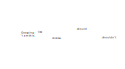
\includegraphics[width=\linewidth+18mm]{./manuscript/tex/diagrams/grasping-turbulence.pdf}

\bigskip

{\small
Turbulence in obstructed water flow.
The formation of vortices is similar to how grasping 'I am' in the mind
causes one to be stuck in a back-and-forth motion between opposite positions.
Fluid simulation by Amanda Ghassaei (\href{http://apps.amandaghassaei.com/VortexShedding/}{apps.amandaghassaei.com}).
\par}
\end{figure}

% FIXME TODO translate figure caption

\vfill\null

\clearpage

\section{Szálak}

\keywords{a szutták mint irodalom}

\noindent A Buddha idejében az irodalom egyik formája a \emph{szutta}
volt, ami egy párbeszéd szálat jelent. A szutták tartalmazhatnak prózai
és verses szöveget is, azzal a szándékkal, hogy szavaláson keresztül
lehessen őket memorizálni. Egy jelentős eseményt követően a szerzetesek
közössége összeállított egy szuttát, ezzel formális alakba öntötték a
történetet és memorizálták azt. Erre a Buddha is szorgalmazta őket:

\begin{quote}
Így kell gyakorolnotok: `Jól oda fogunk figyelni, amikor a
tanítóbeszédeket recitálják, amelyek a Tathágata mélységes, mély
jelentésű, páratlan, az ürességre vonatkozó szavai. Hegyezni fogjuk a
fülünket, kitárjuk a szívünket a megismerésük felé. Úgy tekintünk rájuk,
mint amit megéri megragadni és a mesterévé válni.'
(\href{https://a-buddha-ujja.hu/sn-20.7/hu/fenyvesi-robert}{SN 20.7})
\end{quote}

Manapság a könyvek, cikkek, blog posztok töltenek be hasonló szerepet,
hogy tovább adják a megválogatott információt. Ezek a modern média
anyagok, mikor legjobb formájukat hozzák, a kánon szuttáit tartják maguk
előtt példaként. A korai idők szerzetesei ezeken a szálakon keresztül
juttatták el hozzánk üzenetüket, ez részévé válik az egymás közötti
párbeszédünknek azokkal, akikkel ma találkozunk, és írott munkáink
azokhoz szólnak a jövőben, akikkel mi már nem találkozunk.

\clearpage

\keywords{szociális hálók, szelekciós részrehajlás, Instagram Effektus}

A mai szociális hálókon az üzenet világos megértését torzítja az
úgynevezett `Instagram Effektus', ami egy szelekciós részrehajlás afelé,
hogy csak a legjobb és legpozitívabb oldalunkat mutassuk, és szűrjük ki
a negatívat, ami ennek ellenére éppen olyan valóságos és szükséges a
teljes megértéséhez.

Ez a befolyás nem elhanyagolható. Az orvosi tanulmányok már elkezdték
tárgyalni a depresszió és kényszeres viselkedés egy ide kapcsolódó
formáját, az ún. `Snapchat Diszmorfiát'.\footnote{\href{https://www.ncbi.nlm.nih.gov/pmc/articles/PMC5933578/}{Is
  ``Snapchat Dysmorphia'' a Real Issue? (ncbi.nlm.nih.gov)}} Ezekben az
esetekben az adott személy plasztikai sebészeti kezelést keres, hogy
külsője jobban hasonlítson az alkalmazásban látott mosolygó
fényképekhez.

Az app automatikus szűrői minden képet megváltoztatnak hogy vonzóbbá
tegyék, és ha az app ismételten úgy mutatja nekünk a saját testünket
mint egy szinte tökéletes kép, \emph{az} válik a mentális ön-képünkké,
és a szűretlen kép amit a tükörben látunk, helytelennek fog tűnni.

Egy hasonló Instagram Effektust vehetünk észre a meditációról szóló
cikkekben. A szerzőnek van egy mondandója, amihez a saját
tapasztalatából választ egy szeletet, hozzátéve a véleményeit és más
szerzők magyarázatát.

\enlargethispage*{\baselineskip}

A szerző írhat igazság-hűen és próbálhatja elkerülni az szelekciós
részrehajlást, de valamilyen szűrő mindig működésben van. Az írott szó
világa mindig egy felépített valóság. Viszont, mikor sikeresen eléri
célját, a jól megválasztott szavak nyomán ráismerünk a saját
tapasztalatunkra.

\clearpage

\keywords{mentális képeink mint példaképek}

A meditáló, aki a fejünkben él olyan, mint egy versben szereplő
karakter, vagy egy mítoszban szereplő hős. Hőseink bölcsebbek és
erősebbek nálunk, így amikor elveszettnek és gyengének érezzük magunkat,
hitet és tanácsot adnak nekünk. Az ő békéjük megrendíthetetlen, így
amikor pocsékul érezzük magunkat, képesek vagyunk kiállni azt és várni,
amíg a nehézség véget nem ér.

Az ilyen felépített mentális képek viszont nem mások, csak éppen azok,
nem tekinthetjük őket valódi személynek. Értékes források amikkel
önmagunknak irányt mutathatunk, a történetük leírása segít kitalálnunk
mit tegyünk, azáltal, hogy megmutatja hol vagyunk egy nagyobb kép
keretén belül.

Egy mentális kép szerepe nem az, hogy meghatározza \emph{mivé kellene
váljunk}. Amikor így viszonyulunk a képekhez és ideálokhoz,
önellentmondásokba keveredünk és elégtelennek érezzük magunkat, mert az
élet valós körülményei sokkal összetettebbek, képlékeny és változó
határai mozgásban vannak, nem úgy mint egy kép egy helyben álló,
leegyszerűsített valósága. A képek a magyarázat eszközei. A világra
tekintő \emph{látásmódot} nyújtanak, és példát a helyes cselekvés
irányára az adott fajta világban.

\clearpage

\section{Feltevések}

\keywords{az elme és a világ, a figyelem módja, tettek és hitek}

\noindent Felidézhetjük a Dhammapada verset, ami rámutat, hogy a
tapasztalatunk világa nem független tőlünk:

\begin{quote}
Az elme minden létállapot előtt jár, az elme vezeti őket, az elméből
származnak.

\emph{Manopubbaṅgamā dhammā, manoseṭṭhā, manomayā.}

\bigskip

\quoteRef{%

\href{https://suttacentral.net/dhp1-20/pli/ms}{Dhp 1}

}
\end{quote}

Ez azt jelenti, hogy képzeletbeli problémákat gyártunk magunknak?

Kezdhetjük a vizsgálatot ezzel a kérdéssel: `Képes az alany szenvedést
tapasztalni?' Élőlények szenvedhetnek, de egy kulturális fogalom, vagy
magunk által létrehozott történet nem tud szenvedni, még ha közben
\emph{mi} szenvedünk is. Megváltoztatja a hozzáállásunkat, ha az
aggodalmunk tárgya csak történetként létezik, mint egy intézmény,
nemzet, pénz, hírnév vagy egyéb társadalmi történet, és nem egy élő
lény.

Következő, egy gyors morális biztonsági teszt: `Egy bölcs ember vajon
dicsérné vagy kritizálná ezt?'

Folytatva, felszínre hozhatjuk a nézetünket: `Milyen feltevés hozza
létre ezt a feszültséget és nyomást? Mi ad jelentést nekem ahhoz, hogy
ezt tegyem? Mi az, ami nélkül ennek nem lenne jelentősége?'

Feltárhatjuk az ilyen tudattalan motivációkat azzal, hogy a jelen
tetteinket és választásainkat figyeljük. Amit most választunk megtenni,
kifejezi azt, amiben hiszünk, a korábban elfogadott feltevéseinket.

`Miért választom megtenni ezt, itt? Honnan ered ez a tett és hova
vezet?'

A mögöttes tényezők eredhetnek például a környezetünk által kondicionált
szokásokból. Talán sosem fejeztük ki gondolatban miért tesszük amit
teszünk, de azt éreztük, hogy \emph{az eredmények kifejeződnek rajtunk},
legyenek azok jók vagy rosszak.

A tettekkel kezdeni a vizsgálatot és úgy rákérdezni a gondolatokra egy
eredményes módszer. A belső csevegésünk közben mindenféle belső
ellentmondásokat mondunk magunknak, viszont a tetteink világos
referencia pontokat adnak.

\keywords{a legjobb hely a tanulásra, megfordítani a feltevéseket}

A hozzá kapcsolódó érzés lehet, hogy pocsék, de ha ezt jelzésként
kezeljük arra, hogy forduljunk az elme felé és vizsgáljuk azt, a
hozzáállásunk gyakorlatias és eredményes marad. `Ha már egyszer itt
vagyok, mit tanulhatok ebből?'

A feltevéseinkhez azon keresztül találunk hozzáférést, hogy felfedjük a
tudattalan motivációinkat. Ha egyszer már tisztán ki tudunk fejezni egy
feltevést, szabadságot nyerünk arra, hogy megfordítsuk, vagy elhagyjuk
azt.

Megkérdezhetjük, `Segít ebben a helyzetben, ha megfordítom a
feltevéseimet?' Talán az, hogy az ellenkező irányból tekintünk rá, éppen
az, ami a megbékéléshez kellett, vagy ahhoz, hogy felhagyjunk az üggyel
mint ami sosem létezett. Akárhogy is, már nem kényszerből cselekszünk:
szabadok vagyunk elengedni vagy \emph{választani} azt, hogy végig
folytatjuk.

\clearpage

\section{A Vihar Után}

\keywords{boldogság és sikerek}

\noindent A meditációs útmutatók azt mondják, `térj vissza a jelen
pillanathoz', de ez nem jelenti, hogy mindent szeretned kell amit ott
találsz. A lényeg, hogy ez az egyetlen hely ahol élni tudsz. Ha boldog
vagy, nem a jövőben vagy boldog, hanem a jelenben. Ha szenvedsz, nem
értheted meg a jövőben, csak a jelenben. Egyes helyzeteket semmilyen
agyalás és belső párbeszéd nem fog javítani, legjobb úgy nevezni ahogy
az van, és sztoikusan kivárni a vihart. Egy konfliktus valóban feszült,
elválni attól amit szeretünk szomorú, és életben lenni mindig a saját
halálunk tragédiájával végződik.

Hajlamosak vagyunk a sikert várni, és számítunk arra, hogy a kemény
munkánk a jövőben igazolódik. Vedd szemügyre óvatosan a siker
pillanatát, mit tapasztalsz? Lehet meglepetés, öröm, vidámság,
megkönnyebbülés, ami után minden visszatér a hétköznapi szintre. A
célról kiderül, hogy nem akkora megváltás, mint ahogy gondoltunk. Ha
intenzíven arra koncentráltunk, hogy oda jussunk, talán nem is
emlékszünk semmire az odavezető útról, és azon töprengünk hova tűnt a
sok idő. Olyan erősen leköt minket az, hogy eredményesek legyünk, hogy
elpazaroljuk a lehetőségünket arra, hogy éljünk.

\keywords{értékek, elfoglaltnak lenni, Hedonikus Taposómalom, kiégettség, megelégedettség}

\enlargethispage*{\baselineskip}

A halál felett szemlélődni egy igazmondó, noha kissé ijesztő, tükröt
tart az értékeink elé. `Ha ma este meghalok, boldogan emlékeznék arra,
hogy úgy élek, ahogy ma teszem?' Ez a kérdés többet fel tud kavarni a
psziché mélyből, mint szeretnénk. Emlékszem olyan időre, mikor a
reakcióm a `boldog' szóra kizárólag harag és önutálat volt.

A `Hedonikus Taposómalom' kifejezés leírja az adaptív folyamatot, amiben
minden új sikeres eredményt a pszichénk az új normának tekinti, és egyre
kisebb érzelmi hatást érzünk a céljaink elérése után. Mintha
taposómalomban járnánk, nem számít milyen erősen próbálja az ember
növelni a boldogság szintjét azzal, hogy a következő sikeres lépésre
törekszik, az ember továbbra is egy helyben marad. Az életünket azzal
töltjük, hogy az úton utazunk, nem a célállomásban nyaralunk. Ha
közelebbről megnézzük, még a célállomás puszta ötlete is szétfoszlik,
minta mikor berepülünk egy felhőbe. `Azt hittem ott látom, de most, hogy
ott vagyok, itt semmi sincs.'

Ennek ellenére úgy tűnik, továbbra is azt gondoljuk, hogy elfoglalni
magunkat, eredményesnek és hatékonynak lenni valahogy majd meg fog
minket menteni. Az egyik projekt befejeztével azt érezzük,
\emph{szükségünk van} egy másikra, mert elfoglaltnak lenni a létezés
egyetlen módja, amit ismerünk.

Az öreg bölcsek egyre ismétlik üzenetüket a megelégedettségről, de úgy
látszik el kell szenvedjük a kiégés fájdalmát, mielőtt felfogjuk mi az a
probléma amiről beszélnek.

Bertrand Russell felállítja a diagnózist: `A közeledő idegösszeroppanás
egyik tünete az a meggyőződés, hogy az ember saját munkája szörnyen
fontos.'\footnote{\href{https://www.goodreads.com/book/show/51783.The_Conquest_of_Happiness}{The
  Conquest of Happiness by Bertrand Russell}}

\clearpage

\begin{figure}[h]
\caption{Achievements and the Hedonic Tredmill}\label{fig-hedonic-treadmill}

\centering

\includegraphics[width=80mm]{hedonic-treadmill-stairs.pdf}

\bigskip

{\small

The Hedonic Treadmill is the tendency for new achievements to be adopted as a modified, /normal/ baseline,
and for our level of happiness to return to the same level as before.
After one desire is satisfied, the conditioned craving seeks a new state.

\bigskip

The person on the Penrose Stairs thinks that
they are getting further and higher.
From our outside perspective,
we see that they are merely returning to the same level as before.

\bigskip

Recall the definition of Noble Truth of the Origin of Suffering:
`It is this craving which leads to renewed existence,
 accompanied by delight and lust, seeking delight here and there;
 that is, craving for sensual pleasures, craving for existence,
 craving for extermination.'
(\href{https://suttacentral.net/sn56.11/en/bodhi}{SN 56.11})

}

\end{figure}

% TODO FIXME translate figure text

\clearpage

Henry D. Thoreau kis fakunyhójában Walden Tó mellett azt írja: `Nehéz
dolog, ha déli hajcsárod van; még rosszabb, ha északi; de a legrosszabb
mind közül, amikor te vagy önmagad rabszolga hajcsára.'\footnote{\href{https://www.goodreads.com/book/show/16902.Walden}{Walden
  by Henry David Thoreau}}

Mi lenne, ha a \emph{szabad létezést} gyakorolnád, ahelyett, hogy
gyakorolsz azért, hogy \emph{szabaddá válj}? A fokozatos képzési
rendszer amit a Buddha kifejtett, -- miközben bátorít arra, hogy
szorgalmas erőfeszítést tegyünk a gyakorlásban -- a jelenbeli örömmel
kezdődik, ami megelégedettségből születik a morális- és érzéki
visszafogottságon keresztül.

\begin{quote}
{[}\ldots{]} Vigyáz az érzékeire, védi az elme tényezőit, visszafogja
azokat. Amikor birtokában van ez a nemes érzéki visszafogottság, nem
kifogásolható boldogságot tapasztal magában.

\bigskip

\quoteRef{%

\href{https://a-buddha-ujja.hu/mn-38/hu/a-pali-fordito-csoport}{MN 38},
A szomjúhozás kioltása

}
\end{quote}

\keywords{ön-ellenszenv, ön-kritika, tükrök labirintusa}

Könnyen túl-korrigáljuk a nyüzsgést, és átesünk a másik végletbe:
`Elegem van! Megszabadulok mindentől!' Ez ``logikusnak'' tűnhet, de az
ellenszenvtől hajtva tovább szenvedünk. Sokan vagyunk, akik könnyen
kritizáljuk magunkat, és szorgalmasan gyakoroljuk ezt, olyan
meggyőződéssel igyekszünk bebizonyítani a saját tévedésünket, mintha az
ön-ellenszenv egy erény lenne.

`Pocsékul érzem magam, aki \emph{valóban} tud meditálni sosem érezné így
magát. Biztos, hogy valamit rosszul csinálok.' Egy egész ön-azonosságot
fel lehet építeni ekörül, egy szüntelen belső monológot ami mindig
panaszokkal és ön-ellenszenvvel válaszol. Az ember évtizedeken át élhet
így, és ez válik az alap szintté, ami alapján felismerjük magunkat. `Ha
nem lennék ilyen mérges, nem is ismernék magamra.'

Olyan ez, mint beragadni egy tükrökből készült labirintusba: bárhova
nézel, csak magadat látod. A menekülés kulcsa, hogy találjunk egy
repedést a tükrökön és ismerjük fel a változást: ez a hajtott érzés, a
szorongás és harag motivációi amikről azt gondoltuk állandóak, valójában
folyton változnak -- szétesnek és újra formálódnak. A labirintust az
elme hozta létre, és amit létrehozott üres az éntől. Ez nem lehet az,
ami valójában mi vagyunk.

Kétségtelen, hogy tudunk meggyőző logikát találni az ön-meghiúsító
gondolatainkban, és érvelésünk a kritikus hozzáállásunk védelmében
teljesen észszerű is lehet! A pszichológusok azt mondják, hogy a
legnehezebben kezelhető betegeik azok, akik intelligensen védik és
indokolják saját rossz szokásaikat. Olyan okosak vagyunk, abszolút semmi
esély arra, hogy boldogok legyünk \ldots{} és be is tudjuk bizonyítani!
Emlékszel magadra, mikor az ilyen keserű filozófus szerepét játszottad?

Nem szükségszerűen jelent azonnali megkönnyebbülést, amikor
ön-vizsgálatunk felfedi előttünk az eddig keresett értékeink ürességét.
A harag, kétségbeesés\footnote{A Buddha a haraggal és kétségbeeséssel
  való küszködést ahhoz hasonlítja, mintha egy ösvényt követnénk, ami
  mellett mély szakadék tátong.
  (\href{https://www.accesstoinsight.org/tipitaka/sn/sn22/sn22.084.than.html}{SN
  22.84})} és szomorúság gyakran az első reakciók, és önutálattal
foglalkozó gondolatokat generálnak. Az elmét az elmével tisztítjuk meg:
Ezek az elme állapotok nem megbízhatóak, blokkolják az
intelligenciánkat, és azt ki akarja? Így elengedjük.

\keywords{türelmes kitartás, hála érzet, sietség nélkül}

A türelmes kitartás egy alábecsült erény, de gyakran nincs másra
szükségünk, csak hogy eszünkbe jusson várni: a kavargó elme állapotok
drámai mennydörgése ki fogja magát futni.

Amikor megjelenik a hála érzete, az olyan jel, mint a vihar utáni
szivárvány. A jótékony elme állapotokat kíséri, és intelligensen több
szögből is látjuk a helyzetet. Ez egy jó alap arra, hogy segítőkész
gondolatokat építsünk arról, hogy mit tegyünk. Néha az a legjobb, ha
egyszerűsítünk és elfordulunk bizonyos régi szokásoktól és értékektől.
Máskor, már megváltozott a nézetünk, és talán tovább folytatjuk amivel
eddig foglalkoztunk, de hátra hagyjuk a nagy sietséget. Azért
folytatjuk, hogy azt éljük, nem valamilyen emelkedett elmeállapotra
várunk a jövőben.

\begin{quote}
A múltat ne kergesd,\\
és ne álmodozz a jövőről.\\
Ami elmúlt az már mögöttünk van.\\
Ami eljön azt még nem értük el.

\bigskip

\quoteRef{%

\href{https://suttacentral.net/mn131}{MN 131}, Bhaddekaratta Sutta

}
\end{quote}

\clearpage

\section{Humor és Irónia}

\keywords{vélemények, változó nézőpontok, észrevenni a kellemeset}

\noindent A mogorva, sötét hangulatok olyanok, mintha magunk készítette
logikai csapdák lennének. Minél többet gondolkodunk róla, annál
mélyebbre süllyedünk bennük.

A humor és irónia éppen azért vicces, mert váratlan, furcsa szögből
mutatják a helyzetet. Ha a logikus út egyenesen előre el van zárva,
miért ne próbáljuk meg az oldalcsapást ahol a róka jár? Egy vicc nem
lenne vicces ha logikus és észszerű lenne. A humor és irónia, önmagunk
felé irányítva, jó barátnak bizonyulnak, amikor nem tudunk szabadulni a
saját gondolataink szenvedésétől.

Mitől lesz az öreg és bölcs ember \emph{bölcs}? Orvosi
tanulmányok\footnote{\href{https://www.researchgate.net/publication/258190619_Aging_irony_and_wisdom_On_the_narrative_psychology_of_later_life}{Aging,
  irony, and wisdom, William Randall (researchgate.net)}} megvizsgálták
az idős emberek különféle szemléletmódjait, és azt találták, hogy a
hajlamosság az önmaguk felé irányított humorra és iróniára (vagyis
amikor az ember képes nevetni önmagán) nagy segítséget jelent abban,
hogy szembenézzenek az öregedés jelentős kihívásaival, megőrizzék
szellemi egyensúlyukat és pozitív hozzáállásukat az élethez.

Egyik központi megfigyelésük az, hogy a humor és irónia fejleszti a
képességünket abban, hogy önmagunkat többféle nézőpontból is lássuk.
Egyidejűleg betölthetjük a pontos történész és a tréfáló komédiás
szerepét. Így többféle narrátori szögből is tudjuk látni az eseményeket,
és nem ragadunk be egyetlen történetbe. A narrátori keret amiben
magunkat látjuk, nyitott marad, és egy pozitív jövő irányába halad. A
létezésünk korlátai nem szükségszerűen jelentik a történet végét, és egy
jó nevetésért nem kell messzire menni: az élet abszurd sarkairól mindig
lehet egy jó viccet mondani.

Talán érzéketlen dolog valaki más rossz helyzetéről viccelődni, de ki
fog felháborodni a magadról szóló humoros megjegyzéseidről? Ha pocsékul
érzed magad, mit szólsz egy pocsék vicchez? Ez a menet olyan rossz, hogy
az már jó, és a jegyek ingyen vannak. `Mi vagyok én? Egy életre kelt
csontváz, egy bőrzsákban amire ruhákat aggatok, mesés frizurám alatt a
\emph{fontos véleményeim} logikáját bizonyítgatom.' Hol nincs ezen
nevetnivaló?

Gyakran mondjuk, hogy meditáció közben megfigyeljük a mentális
szokásainkat, de néha ezt egy kritikus elfogultságával gyakoroljuk:
megfigyeljük a \emph{rossz mentális szokásainkat}, és nem vesszük észre
a jókat. Annyira jók tudunk lenni abban, hogy figyelmen kívül hagyjuk a
kellemes elme állapotokat, hogy az ember őszintén elhiszi, hogy a
boldogság csak mások számára létezik. Amikor valami jó történik és
boldognak érzed magad, állj meg és vedd észre, `Na, ez milyen jó.' Ez
növeli a felfogó képességünket arra, hogy a jövőben is észre vegyük és
megtapasztaljuk a hasonló elme állapotokat. Ki fogja észre venni, ha te
nem?

\clearpage

\section{Elvárások}

\keywords{a Buddha szobrok szimbóluma, változó előrejelzések, eloldódás, elhagyás}

\noindent Az ember ránéz egy Buddha szoborra, és talán azt várja el
magától, hogy hasonlóan tökéletes testtartással meditáljon egyetlen
mozdulat nélkül, akár csak a Buddha. Ebben az esetben viszont
félreértettük a szobor üzenetét, ami belső tulajdonságokra mutat, nem
külső jelekre.

A Buddha szobrok nem a történelmi \emph{Sziddhárta Gótamát} ábrázolják,
aki az i.e. 5. században élt. Nem készült róla szobor az élete alatt. A
szuttákból tudjuk, hogy normális magasságú volt és szép küllemű, de arra
utasította a szerzeteseket, hogy ne a testi megjelenésével
foglalkozzanak, hanem a Dhammára, az elme igazságaira fordítsanak
figyelmet.

Azt tanította, hogy még ha egy szerzetes a csuhája sarkába kapaszkodva
követi, de nem látja a Dhammát, nem látja a Buddhát.\footnote{\href{https://suttacentral.net/iti92}{Iti
  92}, A Csuha Sarka} Az első Buddha szobrokat négy vagy ötszáz évvel a
halála után készítették a görögök, az afganisztáni Gandhára régióban. A
Buddha szobrok a felébredett elme bölcsességét és nyugalmát jelképezik,
az emberi formában kifejezve azt.

Gyönyörű rájuk nézni, de senki nem fog Buddha szoborrá válni, mint ahogy
nem válhatsz a tökéletes meditáló képévé sem, vagy a hőssé egy lírikus
költeményben. Tanácsot valóban adnak, de a tanács nem tud irányba
igazítani, ha mereven értelmezzük. Úgy kell alkalmaznunk, hogy
figyelembe vesszük a belső tapasztalatunkat és jelen helyzetünket. Így
visszatérünk a tudathoz, ami ráébred az igazságra és túllép az
akadályon. Az erény gyakorlása és a bizalom a nagy képességű tanítók
példájában erős alapot képez. Jót kívánhatunk magunknak, miközben el
tudjuk ismerni, hogy pocsékul érezzük magunkat, ha éppen olyan a
helyzet.

Az elvárások előrejelzik egy eredmény elvárt értékét, előre megbecslik a
helyzetünk kimenetelét. Eközben, minden tényező ami beszámít az
előrejelzésbe folyamatosan változik. Engednünk kell az előrejelzést is
változni, elvárásainknak a mentális tapasztalatunkról folyamatosan
változniuk kell aszerint, hol állunk éppen most. Az nem jelent
problémát, hogy elvárásaink vannak, de ha ragaszkodunk egy bizonyos
változathoz amit `az igazinak' hiszünk, éppen az válik akadállyá. Az
derül ki, hogy ha jövőbeli érzelmi állapotokba fektetjük a boldogságunk
alapját, az eredmény többnyire a csalódás.

Az \emph{ánápánaszati} légzés meditáció technikáját a Buddha tizenhat
lépésben tanította. Az első, hogy tudatosítjuk, a légzésünk hosszú-e
vagy rövid. Mi az utolsó lépés? Kíváncsian várhatjuk, `Mi lehet az a
fenséges elme állapot, amit végül magunkénak tudhatunk?' A légzésre
irányuló éberség meditáció a test, az érzések, és az elme állapotok
szemlélete után a természetes igazságok szemléletét tanítja, melynek
utolsó lépése:

\begin{quote}
`Az eloldódás fölött szemlélődve lélegzem be, így gyakorol. Az eloldódás
fölött szemlélődve lélegzem ki, így gyakorol.'

\bigskip

\quoteRef{%

\href{https://a-buddha-ujja.hu/mn-118/hu/farkas-pal}{MN 118},
Ānāpānasati Sutta

}
\end{quote}

A Nemes Nyolcrétű Ösvény gyakorlása nem a halmozásról szól, hanem az
értékeink átalakulásáról, a belátáson keresztül a körülmények
változásának tapasztalatába. Végül eloldódunk tőlük, elhagyjuk őket,
mintha letennénk egy terhet, nem cipeljük azt tovább. Ebbe minden
beletartozik, amit az `én és enyém' magába foglal: Meddig tudunk bármit
is megtartani?

\keywords{valódi gyakorlók, Imposztor Szindróma}

A vizsgálódás és fejlődés szélesebbre tárja a látóterünket, amiben az
ellentétek együtt tudnak létezni összetett kapcsolatokban. Az ellenkező
megközelítésben, a bíráló és ítélkező elme egy korlátozott körben mozog,
ami korlátozza a hatáskörünket. Az ilyen látásmód minden dolgot
rendszerezni akar szabályos, egymást kölcsönösen kizáró absztrakt
kategóriákba, ami bizalomvesztéshez és ártalomhoz vezet. Elkezdünk hitet
veszíteni, nem hisszük magunkról, hogy `valódi' gyakorlók vagyunk, és
egyúttal mások sem tűnnek hitelesnek. Az eredmény, hogy nem csak mi
magunk nem tudunk tanulni, de senkit sem tudunk elfogadni, hogy tanítson
minket. Ez a kétség megvakít és megbénít, úgy érezhetjük nem vagyunk
képesek semmit tenni. A probléma az, hogy az elvárásaink túl szűk
területre összpontosítanak.

Nem arról van szó, hogy ne lennének problémák és nehézségek. Azt
magyarázni magunknak, hogy a fájdalom nem fájdalmas, nem olyan
meditációs technika amit a Buddha tanított. Viszont nem kellene
feltételezzük, hogy olyannak kell lennünk mint a mitológiai ideáloknak.
A meditáció nem egy kapcsológomb, amivel irányítani tudjuk az elme
állapotokat, hanem a tudatosság fejlesztése, hogy az elme állapotok ne
irányítsanak minket.

\section{Érzelmek Kalibrálása}

\keywords{új érzelmeket tanulni, variáció a normális, csalódás, saññā és saṅkhāra}

\noindent Amikor egymásnak az érzelmekről beszélünk, gyakran úgy
magyarázzuk meg a működésüket mint egy `idegrendszeri áramkör', vagy az
agynak egy területe, ami bizonyos helyzetekben aktiválódik. Eszerint a
történet szerint, egyes agyterületek születésünktől fogva be vannak
kötve adott érzelmek kiváltására, és emiatt érzünk félelmet, szeretetet,
haragot vagy undort.

De akkor hogyan magyarázzuk, amikor valaki, akinek hiányzik az
\emph{amygdala} területe, mégis tapasztal félelmet? Az \emph{amygdalát}
jellemzően felelősnek tekintjük erre az érzelemre. Vagy mi a helyzet a
kifinomultabb kategóriákkal?

A japán `\emph{mono no aware}' jelentése a mulandóság miatti szomorúság
és ebben talált szépség érzése, a japánok vajon ilyen idegi áramkörrel
születnek? A leírás alapján talán magad felismered az érzést, ha láttál
japán filmeket, még ismerős is lehet, és most, egy szóbeli kifejezést
ráillesztve egyre könnyebben érezheted.

Más kultúrák a nyugati érzelmeket találják furcsának, mint például az
Utka eszkimók, akiknek nincs a `harag' koncepcióra közvetlen
megfelelőjük. Vagy a tahitiak, akiknek nincs `szomorúság'-nak megfelelő
képzetük.

\enlargethispage*{\baselineskip}

Az orvosi tanulmányok arról számolnak be, hogy semmilyen érzelemnek
nincs születéstől fogva beépített `áramköre'.\footnote{\href{https://www.goodreads.com/book/show/23719305-how-emotions-are-made}{How
  Emotions Are Made: The Secret Life of the Brain by Lisa Feldman
  Barrett}, Theory of Constructed Emotion} Nem az adott érzelem
alapvető, hanem a képességünk, hogy felismerjük a veszteség és nyereség
mintáit, hogy \emph{megtanuljunk érzelmi koncepciókat} más emberektől,
és felismerjük azokat egy új helyzetben a jövőben.

Egy adott helyzetben, az agy felismeri, hogy egy korábbi tapasztalat
\emph{egy ehhez hasonló kontextusban} nyereséggel járt vagy sem. Ez
idővel könnyebbé válik, ha megtanultunk hozzá társítani egy érzelmi
koncepciót, és ezzel spontán, automatikus érzéssé válik.

Egy érzelem kategória adott esete változó jellemű: a `félelem egy
tigristől' különbözik a `félelem egy vizsgától' érzéstől, melyek tanult,
adaptív előrejelzések. Csak bizonyos mértékben illeszkednek, mint ahogy
egy személyre ráilleszthető egy sztereotípia, de nincs olyan személy,
aki 100\%-os példája egy sztereotípia minden jellemzőjének.

Az agyunk kiértékeli a jelent a múlt alapján, és annak megfelelően, hogy
jó vagy rossz várható, egy választ érzünk a test különböző részein, és
ebből egy érzelem esetét alkotjuk a meglévő koncepcióink alapján.

\keywords{az érzelmek nem precíz mentális tárgyak, érzelmek tanulása, metta és sukha, mi a baj velem}

Az érzelmek klasszikus nézete szerint -- amihez hétköznapi
beszélgetésben vagyunk szokva -- az érzelmeket úgy kezeljük, mint
precízen mentális tárgyakat. Az elképzelés az, hogy egy érzelemnek
tisztán meghatározható jellemzői vannak, amiben két szellemileg
egészséges ember meg kell tudjon egyezni.

Viszont miközben az agyat működés közben tanulmányozták, nyilvánvalóvá
vált a tudósok számára, hogy ez semmiképpen nem lehet így. Ahogy egyre
több vizsgálatot végeztek, a bizonyíték folyton ellenkezett ezzel a
nézettel.

Amikor az emberek testi és pszichológiai teszteken mentek át, amiben
érzelmeiket vizsgálták, az eredmények nagyban különböztek az egyének
között. Nem volt semmilyen jól meghatározható, tisztán látható jelzés,
vagy `ujjlenyomat', ami beazonosíthatta volna bármelyik érzelmet.
Ehelyett, a \emph{változatosság volt a normális}, mind az egyének
érzelmi tapasztalataiban, azon érzelmek jelentésében és céljában, és az
ennek megfelelő testi reakciókban.

A tudósok azt találták, hogy a test és az agy \emph{megtanulja} az
érzelmi kategóriákat az észlelések kondicionáló folyamatán keresztül.
Saját kultúránkból, más emberektől akikkel együtt élünk (társadalmilag
kondicionált érzelmek); biológiai szükségleteinkből (testileg
kondicionált \textasciitilde); vagy személyes élményeink alapján, mint a
régi szokások, jelentős események és emlékeink.

Ez ahhoz is kapcsolódik, hogy egy adott személy nem mindig érti, vagy
talán fel sem ismeri egy másik ember érzelmeit. Gondolj például a
kultúr-sokkra, amikor egy távoli országba utazol: egy érzelemnek, mint a
`szeretet', változatos kifejezési formái vannak, olyan kontextusai és
mögöttes feltevései, amik nem voltak részei a saját érzelmi
kategóriánknak a `szeretetre'. Eltarthat egy ideig, amíg hozzá szokunk
az új jelekhez és jelentésekhez, ráérzünk az árnyalt különbségekre, és
megbízhatóan fel tudjuk ismerni a jeleket másokon.

Kérdezd meg magadtól, honnan tudod, hogy egy adott érzelmet érzel, mint
a \emph{metta} (szerető kedvesség) vagy \emph{sukha} (boldogság)? A
modell, amit érzéseink megértésére használunk, befolyásolja mit várunk,
hogy meditációs gyakorlásunk alatt történjen. Ha az érzelmekre úgy
tekintünk, mint határozott dolgokra, mintha külső tárgyak lennének amit
reprodukálnunk kell, vagy hozzá kell férjünk, könnyen úgy fogjuk érezni,
`ez nem az, nem tudom mi a baj velem.'

Mivel a \emph{változatosság a normális}, saját tapasztalatunk
valószínűleg különbözni fog másokétól. Az egyéni meditációs
tapasztalatok olyan változatosak, mint az egyének maguk. Egy érzelem
adott esetétől várható, hogy eltér az általános fogalomtól. Fontos, hogy
arra támaszkodjunk, hogy ismerjük a \emph{saját} elménket és
érzéseinket, ahelyett, hogy külső leírásokat próbálunk reprodukálni.

A szabadságunk arra is kiterjed, hogy megtanuljunk és létrehozzunk olyan
érzelmeket, amikről korábban nem is hallottunk. Az éberségre támaszkodva
észleljük a tapasztalatunkat, önmagunkat képezzük a koncepcióra, és
megteremtjük a feltételeket az érzelem megjelenésére.

Az Öt Khandha terminológiájával úgy mondhatnánk, hogy az észlelések
(\emph{saññā}) és mentális késztetések (\emph{saṅkhāra}) egymást
befolyásolva megalapozzák a tapasztalat mintáit, amit megtanulunk
beazonosítani mint egy szélesebb, absztrakt érzelmi kategória jelenbeli
esetét.

A külső leírások olvasásával kezdjük, és ezt belső tapasztalattá
alakítjuk át a vizsgálódáson és mindennapos tetteinken keresztül.
Megismerni a tapasztalatunkat referencia pontot ad. Idővel, az új
tapasztalatok ismerőssé válnak és erőlködés nélkül megjelennek.

\keywords{az érzelmek mint előrejelzések, kultúr-sokk, elvárások igazítása}

Az agy folyamatosan kapja a jeleket az idegrendszertől, és az alapján,
hogy mit tanult a múltbeli tapasztalatok alapján, próbálja megítélni,
hogy vajon a jelen helyzet energia bevitelt vagy energia kiadást fog
jelenteni a test számára.

Az agy válaszként felkészíti a tested, mint például növeli vagy
csökkenti a szív ritmust, beindítja vagy megállítja bizonyos hormonok
termelését. Ezt a testi reakciót tapasztaljuk, és ha korábban
megtanultunk egy érzelem kategóriát aminek ez megfelel, az adott érzelem
egy változatát érezzük: a veszélytől való félelem, az azonnal várható
jutalom izgalma, vagy a szárnyaló boldogság.

Ez magyarázza a kultúr-sokkot: ha más kultúrában nőttél fel, más érzelmi
kategóriákat tanultál, és amikor egy távoli országba utazol,
ismeretlennek hathat számodra az ott élő emberek érzelmi világa.

Hajlamosak vagyunk azt hinni, hogy a tapasztalatunk olyan, mint a
látvány amikor kinézünk az ablakon. Az ember `ránéz a tapasztalatára',
és látja mi történik.

Gyorsan kiderül, hogy amit látunk sokkal hiányosabb, mint gondoljuk, ha
meggondoljuk hogyan működnek az érzékek és az idegrendszer. Az agy nem
kap túl sok információt, amivel dolgoznia kell, és néhány egyszerű
jelből meg kell tippelnie, milyen lehet a gazdag világ, ami rajta kívül
van.

Az agy nem lát túl sokat: ott kuksol a koponyában, ami olyan, mint egy
sötét doboz. Testi folyadékok, vegyületek és idegrendszeri jelek
üzeneteket továbbítanak ebbe a dobozba. Az üzenetek a test már
rendszereitől erednek, amik maguk is zajosak és néha egymásnak
ellentmondanak. Ebből a kavalkádból az agynak létre kell hoznia az
észlelt képet arról, hogy hol vagyunk, megtippelnie mi történik velünk,
megjósolnia valószínűleg mi fog történni a következő pár percben, és
produkálnia kell egy választ, ami remélhetőleg segít bennünket a
túlélésben, vagy akár még boldogsághoz is vezethet. Ezt mind egy sötét
dobozon belülről kell véghez vigye, néhány zajos és korlátolt jelzés
alapján.

\clearpage

Mi vagyok tehát? Egy életre kelt csontváz, a fejem pedig egy sötét
doboz? Ez sok zavarodottságot megmagyaráz. Csoda-e, hogy az elvárásaim
egy kicsit félrecsúsznak, és folyamatos igazgatásra van szükségük? Amit
valóságként tapasztalok, egy folyamatban lévő találgatás eredménye, ami
másodpercenként változik.

`A boldogság egyenlő: valóság mínusz elvárások' -- Tom Magliozzi mondása
szerint. Manapság az elvárásaink olyan magasak. Frissítéseket kapunk a
szociális média appoktól, web cikkeket olvasunk, és minden alkalommal
befolyásolják a nézetünket arról, hogy vagyunk és hogy áll a világ
körülöttünk. Tökéletes, elhatározott, felháborító képeket mutatnak
nekünk más emberekről. Mivel nem találkozunk ezekkel az emberekkel
szemtől-szembe, nem látjuk az életük valóságos hátterét, és ez
felnagyítja az elvárásainkat. Ez újra és újra arra képezi az agyat, hogy
ezeket a mesterségesen létrehozott benyomásokat várja el, mint egy
túlhajtott elvárás-gép. Észre sem is vesszük ezt a torzított
ön-kondicionálást, de csalódottak és kimerültek vagyunk, ami szüntelen
elégedetlenséghez vezet.

\keywords{egyszerűség, állandótlanság, ön-vizsgálat, értékek}

Viszont megvan a képességünk, hogy kalibráljuk az `elvárás gépet', a
tudatos vizsgálódás és megfontolás kiegyensúlyozó hatásával. `Mi a
legfontosabb a mai nap? Mire van szükségem ehhez az egy naphoz?' Ha
leegyszerűsíted a választ a lényegre, nem olyan sok. Étel, ruha,
szállás, gyógyszer, támogató szellemű társak és talán valami tennivaló
egy érdemes cél irányába.

Az átlagos nap valószínű, hogy kuszább ennél, és nem igazodik az ilyen
absztrakt, tiszta egyszerűséghez, de ez arra szolgál, hogy felismerjük
az alap szintet. Ha az egyszerű is elegendő, akkor nem jelent problémát,
hogy többet is tudunk tenni, vagy több mindenhez is hozzáférünk, amíg a
megelégedettség marad az alap szintünk. Nem a törekvés a probléma, de az
elvárások felnagyítása blokkolja annak megvalósítását.

Az elvárások szükségesek ahhoz, hogy egy adott irányt kövessünk a
világban, de ha nem értjük őket, akadályokká válnak a szívben. Az
elvárások és érzelmek természete az, hogy megjelenjenek, és ide-oda
fordulva változzanak. Hagyd, hogy tovább ússzanak, mint falevelek a
csónak mellett. A rosszak nem olyan rosszak, a jók nem olyan biztosak.
Ismerve a változó természetüket, nem vesszük őket olyan komolyan, és nem
akadunk fenn bennük, mint ahogy egy csónaknak sem kellene fenn akadnia
holmi leveleken.

\begin{quote}
Legyen kellemes vagy fájdalmas,\\
a semlegessel együtt,\\
Akár belső, akár külső,\\
Bármilyen érzés ami van:\\
Megismeri, `Ez is szenvedésnek van kitéve,\\
megtévesztő és szétbomló',\\
Újra és újra érintve őket,\\
elmúlásukat szemlélve,\\
a szenvedélytől megszabadul.

\bigskip

\quoteRef{%

\href{https://suttacentral.net/sn36.2/pli/ms}{SN 36.2}, Sukha Sutta

}
\end{quote}

\clearpage

\section{Virágzó Élet}

\keywords{a boldogság jelentései, eredmények, egyszerre egy napot gyakorolni, halál, megelégedettésg}

\noindent A modern nyugati kultúránk a boldogságot gyakran úgy mutatja
be, mint egy meghatározott érzés, vagy egy bizonyos élethelyzet ahova el
kellene érkezzünk. Kultúránkat átadjuk egymásnak a közös párbeszéden át.
A boldogságról olyan módon beszélünk, mint egy eredményről, egy
eseményről a jövőben, vagy mint egy bizonyos létállapotról. Úgy tűnik,
ez egy nemrég kialakult szokásunk, és nem egy kifejezetten jótékony
hatású.

Hagyomány szerint az ókori görögökre úgy tekintünk, mint az egyik
legnagyobb befolyású társadalomra a nyugati értékeink kialakulásában.
Arisztotelész (i.e. 384-322) az egyik ilyen nagy befolyású gondolkodó,
és a mai napig olvassuk és visszautalunk a fennmaradt írásaira. Ezekben
a szövegekben részletesen vizsgálja a boldogság kérdését.\footnote{\href{https://plato.stanford.edu/entries/aristotle-ethics/}{Aristotle's
  Ethics (plato.stanford.edu)}} Láthatóan erősen foglalkoztatta, hogy mi
a boldogság, hogyan élhet az ember boldogan, viszont tőlünk eltérően,
nem úgy tekintett rá, mint egy adott eredményre vagy életkörülményre.

\enlargethispage*{\baselineskip}

A görög szó, amivel a boldogságra utal az \emph{eudaimonia}, fordításban
`emberi jólét, virágzó élet.' Úgy látta ezt megjelenni, mint egy
folyamatosan aktív folyamatot, amit nap mint nap gyakorlunk, nem pedig
egy eredményt, amit egyszer majd a jövőben elérünk. A boldogság
gyakorlását a morális erényekre alapozza, és az ember saját életére
vonatkozó valósághű szemléletre, ami a születéssel, a növekedés éveivel,
és az öregkorral együtt magába foglalja az ember saját halálának
tragédiáját.

Az erény és halandóság ilyen közvetlen szemlélete sorba rendezi a
dolgokat: egy tágas nézőpontot ad, amiben a boldogság a jótékony
szellemi tényezők alapjára épül, de önmagunkon túl kell néznünk ahhoz,
hogy hosszú távú jelentést adjunk annak.

Az elvárásainkat így képezve, a boldogság gyakorlata minden nap teljes
egész. Megtanulunk a nehézséggel együtt lenni, ha éppen úgy áll a
helyzet, és legjobb képességünket erényesen alkalmazva minden nap végén
megnyugvással tekinthetünk vissza.

A pszichológia `boldogság kutatás' területén Daniel Kahneman és csapata
interjúkat végeztek, amikben arra kérték az embereket, hogy idézzék fel
az előző napi eseményeket, és később válaszoljanak az erről szóló
kérdésekre.\footnote{\href{https://www.goodreads.com/book/show/11468377-thinking-fast-and-slow}{Thinking,
  Fast and Slow by Daniel Kahneman}, Day Reconstruction Method} A
kiértékelés megerősítette, hogy a figyelem és az ismétlődő gondolatok a
domináns tényezők abban, hogy valaki boldognak vagy depressziósnak érzi
magát. Miközben a jelentkezők különböző hétköznapi helyzeteken mentek
át, nem az határozta meg azt, hogy miként érezték magukat, hogy hol
voltak és mit csináltak, hanem, hogy miről gondolkodtak éppen akkor.

\keywords{megbánás a halálos ágyon, az élet mint idő egység, a szükségletek hierarchiája, ön-megvalósítás, ön-meghaladás}

\enlargethispage*{\baselineskip}

Az viszont meglepetésként érte őket, hogy amikor az emberek arról
beszéltek milyen napjuk volt, nem a boldogságról beszéltek mint egy jó
érzésről, sokkal inkább arról, hogy milyen társasági élményeik voltak,
barátokkal és rokonokkal, kivel találkoztak és mit csináltak együtt, és,
hogy elégedettnek érezték-e magukat az életükkel, vagy sem.

Ez érthető, ha megvizsgáljuk saját tapasztalatunkat: a szemlélet, a
keret amin keresztül a világot látjuk adja meg a tájékozódási
pontjainkat, miközben a keret tartalma folyamatosan változik. Az éhes
ember a világot az ételszerzés szemszögéből látja. Aki célratörő
hangulatban van arra összpontosít, hogy `mire vagyok képes', és `milyen
jó vagyok.' Aki eltöpreng milyen korlátozott idejű a személyes létezése,
hajlamos olyan értékek felé fordulni, amik önmagán túlmutatnak.
Ahelyett, hogy az `én' által létrehozott tapasztalatok foglalkoztatnák,
az ember az időtlen jellemzők felé fordul, amik itt és most láthatóak.

Számomra felfedezés volt, mikor egy interjút hallgattam,\footnote{\href{https://www.samharris.org/podcasts/making-sense-episodes/209-a-good-life}{A
  Good Life: A Conversation with Scott Barry Kaufman}} és hallottam a
pszichológusokat arról beszélni, hogy egy új elemet adtak hozzá Abraham
Maslow ú.n. szükségletek hierarchiájához. Ezt rendszerint egy
piramisként ábrázolják, ami az alsó szinten az étel- és víz
szükségletével kezdődik, majd az ön-megvalósítással végződik, amit a
csúcsra emel. Ez a boldogságról egy meglehetősen én-központú
gondolkodási módnak tűnt.

\enlargethispage*{\baselineskip}

A pszichológusok nemrég újra elővették Maslow későbbi
írásait,\footnote{\href{https://bigthink.com/neuropsych/maslow-self-transcendence/}{Maslow's
  forgotten pinnacle: Self-transcendence (bigthink.com)}} és azt
találták, hogy az élete végéhez közeledve, konfliktusban érezte magát
saját rendszerével az értékek hierarchiájáról: hamarosan meg fog halni,
szükségleteinek alapvető részei (mint a túlélés) hiányoznak, tehát
nyomorúságosan kellene érezze magát, de ehelyett, felszabadultságot és
olyan boldog állapotokat érzett, amit `csúcs-élményeknek' nevezett:

\begin{quote}
Az érzések határtalan horizontja nyílik meg a szem előtt; az érzés, hogy
erőteljesebb, és egyúttal gyámoltalanabb vagy mint korábban bármikor; a
hatalmas eksztázis, csodálkozás és révület érzése; elveszíteni hol vagy
időben és térben; és végül -- a meggyőződés, hogy valami kifejezetten
fontos és értékes történt, mely élmény nyomán az ember részben átalakult
és megerősödött, kihatással a hétköznapi életére is.
\end{quote}

Maslow hozzácsatolt még egy szintet a szükségek hierarchiájához, az
ön-megvalósítás felett: \emph{az ön-meghaladást}. Ennek példái: nem
ragaszkodni a tökéletességhez, nem tartani mereven saját véleményünket,
feladni a bizonyosság szükségét, feladni a saját múltunkhoz való
ragaszkodást, és elengedni a haláltól való félelmet.

Az `ön-meghaladás' úgy hangzik, mint ami egy Buddhának való, de mivel
szenvedünk a ragaszkodásainktól a különféle dolgokhoz, kiderül, hogy ez
mindannyiunknak számára egy alapvető \emph{szükséglet}.

\enlargethispage*{\baselineskip}

A ragaszkodás ahhoz, amiről azt gondoljuk mi vagyunk, hozza létre éppen
azokat a korlátokat, amikkel küszködünk. Egyre szélesebb körű horizontot
akarunk látni, de visszatart minket, hogy egy ön-azonosságba
kapaszkodunk. Amikor arról az azonosságról kiderül, hogy egy üres tér,
sürgős segítségre van szükségünk. Gondolj a mindennapos küzdelmekre:
konfliktusba kerülünk a véleményünk miatt, feszültek vagyunk a
képességeink hiánya miatt, idegesek vagyunk a váratlan változásoktól,
siratjuk a múlt tragédiáit. Szükséges egy ön-meghaladó szemlélet, hogy
túltegyük magunkat magunkon.

\clearpage
\figurepagelayout

\begin{figure}[h]
\caption{Hierarchy of needs, self-transcendental values}\label{fig-self-transcendental}
\bigskip
\includegraphics[width=\linewidth]{./manuscript/tex/diagrams/self-transcendental-values.pdf}
\end{figure}

% TODO FIXME translate figure

\clearpage
\normalpagelayout

Mégis, számon tartjuk hogy állnak a dolgaink az életben, nem igaz? A
jótékony tényezők a támogató alapot jelentik. Ez az a hely és idő ahol
élünk, nem egy másik: \emph{memento vivere}, emlékezz, hogy élj. Tudjuk
magunkról, hogy az erőfeszítéseink összhangban állnak a központi
értékeinkkel vagy sem, még akkor is, ha elterelik a figyelmünket olyan
dolgok, amiken nem terveztünk olyan sok időt tölteni.

Emlékszem engem mennyire felrázott, amikor azt olvastam egy ápolónő
beszámolójában,\footnote{\href{https://bronnieware.com/blog/regrets-of-the-dying/}{Regrets
  of the Dying (bronnieware.com)}} hogy a halálos ágyon mondott
leggyakoribb megbánások közé tartozik a túl sok munkával töltött idő, és
elveszíteni a kapcsolatot a régi barátokkal. Az élet egy idő egység,
aminek kezdete és vége van, és ennek megfelelően kell azt kezeljük.

\keywords{\emph{memento mori}, \emph{memento vivere}, \emph{amor fati}, \emph{saṃvega}, \emph{pasāda}}

Ha az elmét egy kényelmes tompaságban elmeríteni azt jelenti, hogy
`benyugtatózzuk magunkat a triviális dolgokkal', akkor emlékezni a
halálra (\emph{memento mori}) egy adag anti-nyugtatót jelent. Mivel az
idő korlátozott, emlékszünk a sürgetésre, hogy éljünk (\emph{memento
vivere}), és tegyük meg amit kell mielőtt túl késő. Ez motivációt ad,
hogy megtaláljuk a bátorságot arra, hogy igazak legyünk önmagunkhoz, és
forduljunk a helyzet felé amiben élünk (\emph{amor fati}), ne várjuk
valamilyen képzeletbeli helyre és időre a jövőben. A buddhista
szuttákban, páli nyelven a \emph{saṃvega} szó utal a spirituális
sürgetés érzésére, míg a \emph{pasāda} kifejezi a higgadt örömet abban,
hogy meggyőződésünk van az Útban és annak gyakorlásában.

A halálos ágyon mondott megbánásokról olvasni időszerű emlékeztető volt
számomra, hogy gondolkozzak el a sürgető érzésen, amit a projektek
teljesítésére éreztem (amik hónaponként jönnek és mennek), és ne
veszítsem el a lehetőséget, hogy minőségi időt töltsek régi
ismerősökkel.

Az életre úgy gondolni, mint egy adott idő egységre, magában foglalja a
születést, felnövést, megöregedést és a halált. Így emlékezni
halandóságunkra, értékeinket helyre teszi a természet tényeivel
összhangban.

Engedhetünk magunknak időt arra, hogy éljünk ott ahol vagyunk, és
értékeljük azt, mielőtt vége szakad. Úgy tűnik, értjük a jó és rossz
érzések mulandó természetét, mikor összevetjük őket az arany
kapcsolataink fontosságával.

Emlékezzünk, hogy magunknak jólétet és boldogságot kívánunk,
családunknak és barátainknak is boldogságot kívánunk az életükben. A
szellemi kitartást és önbecsülést úgy építjük, hogy tudatosan felidézzük
a morális erényeket. Elismerhetjük magunknak: `Ezt jól tettem. Ez jó
munka volt.' Vagy másokban látjuk, mint tanítók, példaképek és barátaink
esetében.

Ez fejleszti az örömöt és értékelést, amit mások sikerei és jósága
nyomán érzünk, ahogy osztozunk a sikereikben. A boldogság egyik mély
forrása a szemtől-szembeni kapcsolatokat fejlesztenünk olyan barátokkal,
akikkel kölcsönösen átérezzük az élet sikereinek örömét. A humorral
feloldhatjuk a mogorva hangulatunkat, és megtesszük a következő lépést,
ami előre visz.

A jelen maga a változás. Ezt a tapasztalatot éberen figyelve vizsgáljuk
a testet, az érzéseket, elme állapotokat és a dolgok természetes
igazságát a \emph{Szatipatthána Szutta} refrénjét követve:

\begin{quote}
\ldots{} Úgy időzik, hogy a keletkezés természetét szemléli, vagy úgy
időzik, hogy az elmúlás természetét szemléli, vagy úgy időzik, hogy a
keletkezés és az elmúlás természetét szemléli. \ldots{} Szabadon időzik,
semmihez sem kötődve a világon.

\bigskip

\quoteRef{%

\href{https://a-buddha-ujja.hu/mn-10/hu/toth-zsuzsanna}{MN 10}, Az
éberség megalapozásáról szóló tanítóbeszéd

}
\end{quote}

\chapter{Miért}

\section{Kétség és Hit}

\keywords{kényszeres gondolatok, nézetek irányba igazítása, váratlan változások}

\noindent Előfordul, hogy azért érdekel minket a meditáció, hogy meg
tudjunk birkózni egy felkavaró vagy fájdalmas tapasztalattal. Tudjuk,
hogy `valami nincs rendjén', és nem tudjuk lerázni az érzést. Vagy lehet
ez a veszteség fájdalma, ami olyan zavar érzését kelti, amiben látszólag
semminek sincs értelme: az ilyen érzések egyre csak visszatérnek, nem
engedik magukat figyelmen kívül hagyni. Válaszok helyett, csak a
gondolataink járnak körbe-körbe: `Miért kell ennek így lennie? Mit
kellene tegyek, és miért? Mi értelme ennek?'

Még az ilyen zavart állapotban is, pusztán elismerni magunknak a belső
káosz állapotát is már elkezd irányt és rendet teremteni.

Ahhoz hasonlít ez, mintha olyan úton vezetnénk, ami tele van szórva
szeméttel. Lelassítani és körül nézni máris sokkal jobb, mint vaknak
lenni a veszélyes hulladékra. Tele van a fejünk gondolatokkal, de
közöttük kevés mutat megbízható irányba, így jobb, ha megvizsgáljuk
őket. Korábban volt egy elképzelésünk, hogy a dolgok hogy állnak a
világunkban, de ezek megváltoztak olyan módon, amire nem számítottunk.
Nem a dolgok hibája, nem a mi hibánk, de a váratlan változás megzavaró,
és nézetünket igazítanunk kell.

Az állandótlanság kirántja a lábunk alól a szőnyeget, de egyúttal át is
alakítja az értékeinket, azokat a jellemzőket, amiket keresünk és
értékesnek tartunk a tapasztalatainkban. Ha nem értjük a változást, az
zavart okoz, amit kétség követ. Talán tudjuk, mit \emph{kellene
tegyünk}, de a kétség és jelentés nélküliség érzetében elakadunk, és el
sem tudjuk kezdeni.

\keywords{jelentés, vizsgálni mit hiszek, hit mint üzemanyag}

Miért kelsz fel reggel, hogy tegyél bármit is? Miért számít egyáltalán?
Ha folytatom a `miért' kérdéseket, és így beleások a felépített énem
rétegeibe, az első réteg a megszokott rutint tárja fel, `mert ezt
csináltam tegnap is.' Ez alatt, a válaszokat olyan történek formálják,
amiket én mondok magamnak arról a világról, amiben élek. Ez alatt, van
valamilyen érvelés, filozófia és absztrakt ötletek. Ez alatt, kezdek
kétségbeesetten kapaszkodni valami szilárd dologba, és elkezdem
emlékekkel és tapasztalatokkal védeni az elképzeléseimet (`mert amikor
így megy így jártam\ldots{}'), vagy híres személyekre hivatkozok (`mert
ez és az a tanító azt mondta\ldots{}').

Ez alatt, fel kell adjam és bevallanom, hogy a dolog hit és személyes
meggyőződés kérdése. Amit teszek, egyszerűen az, amit eldöntök ott és
akkor. A végén ott állok, hogy \emph{nem tudom, de úgy hiszem}, hogy azt
tenni értelmes dolog.

A hit nem egy rögzített jellemző az elmében, megvan a kapacitásunk, hogy
megválasszuk a hitelt érdemlő állításokat amiket úgy látunk, hogy
nagyobb megismerés és boldogság felé irányítanak minket.
Alátámaszthatjuk, vagy elhagyhatjuk a hitet azzal, hogy gyakorlatban
alkalmazzuk és figyelünk az eredményekre.

Ellenőrizhetem, felülvizsgálhatom és frissíthetem \emph{mit hiszek}
arról, hogy minek van értelme, de amíg a tapasztalatom nem igazolja azt,
az érvelésemet a hitnek kell alátámasztania. Különben nem fogok
erőfeszítést tenni semmilyen irányba, és az életemet vak szokások és
külső nyomások fogja uralni.

A hit az elhatározás és energia erényeinek üzemanyaga. Később, a hitet
megerősíti az, hogy magunkon érezzük a gyakorlás eredményeit, de
üzemanyag nélkül, az autónk el sem indul.

\keywords{hit mint a tett kiváltó oka, bizalom a tanítóban}

A hit okot teremt a tettre. Hit nélkül, nem teszem meg az adott dolgot.
A buddhista látásmódban két alapvető hittétel van:

\begin{enumerate}
\item
  Egy jelenség megtörténik, ha az elégséges feltételek megvannak hozzá,
  és nem történik meg, vagy megszűnik, ha az elégséges feltételek
  hiányoznak.\footnote{\href{https://www.dhammatalks.org/suttas/SN/SN12_61.html}{SN
    12.61}, Tanulatlan}
\item
  A Buddha teljesen megértette az igazságot arról, ahogy a dolgok
  vannak, és így megszabadította magát a mohóságtól, gyűlölettől és
  zavarodottságtól. Emiatt kiváló tanítója a gyakorlás útjának.
\end{enumerate}

A Buddha arra adott utasítást, hogy mindenkinek magának kell
rákérdeznie, töprengenie, és megvizsgálnia azt, hogyan vannak valójában
a dolgok, hogy megértse azt. De mégis, hogyan fogjunk hozzá? A tanítóban
való hit nélkül, el vagyunk veszve a személyes véleményeink
kuszaságában, és nem valószínű, hogy hallgatni fogunk másra és tanulni
valami újat. A hagyomány erre a kapcsolatra emlékeztet minket, amikor
egy Dhamma beszéd előtt, a \emph{namo tassa} sorait kántáljuk háromszor.

\begin{quote}
\emph{Namo tassa bhagavato arahato sammā-sambuddhassa}

Tisztelet a méltóságos Magasztosnak, a saját erejéből tökéletesen
megvilágosodottnak.
\end{quote}

\keywords{kétség, sivatagban bolyongani, a ragaszkodás korlátokat teremt}

A Buddha ahhoz hasonlította a kétséget, mintha egy sivatagban
bolyonganánk víz nélkül.\footnote{\href{https://suttacentral.net/dn2}{DN
  2}, A Szerzetesi Élet Gyümölcsei} Minden más másodlagos, csak arra
tudunk gondolni, hogyan találjunk vizet és jussunk ki a sivatagból.

Vagy, hogyan tompítsuk el az elmét és egyáltalán ne gondoljunk semmire,
`álomba ringatni magunkat a trivialitással'\footnote{Søren Kierkegaard,
  `A halálos betegség'}, hogy mindent úgy folytathassunk mint eddig. A
kétség miatt nem világos, hogyan szabadulhatunk ebből a helyzetből, de
kezdhetjük azzal, hogy elismerjük magunkban a törekvést, hogy jól
legyünk és boldog életet éljünk.

Emberi természetes képességünk, hogy túljussunk a zavaron és hosszú távú
boldogságot fejlesszünk az életünkben. A hosszú távú szemléletnek magába
kell foglalnia a helyzetünk változását, a veszteséget és tragédiát. A
stabil boldogságnak olyan szemléletre kell alapulnia, amely magába építi
az állandótlanságot.

A szuttákban, a kétség szerepel az Öt Akadály listáján is, és Tíz Béklyó
első három eleme között is, melyek eltakarják a Négy Nemes Igazság
megértését. Mikor személyesen érint, nincs kétség, hogy a kétség
szenvedéshez vezet. Az ábrák \ref{fig-leading-to-suffering} és
\ref{fig-leading-to-cessation} illusztrálják hogyan kerülünk ebbe a
káoszba, és hogyan tudunk kijutni belőle.

Mint akadály, a kétség megállítja a Helyes Erőfeszítést, és megállítja
az elme fejlesztését. Mint béklyó, arra késztet, hogy fix
bizonyosságokat keressünk, és így még szorosabban köt minket az
elképzeléseinkhez arról, kik vagyunk.

Szeretjük a javaslatot, hogy fejlesszük az elménket, de kezdetben azt
gondoljuk, ez azt jelenti, hogy megerősítsük kik és mik vagyunk, többet
szerezzünk abból amire szükségünk van, vagy megváltoztassunk magunkat és
valami mássá váljunk.

`Ki vagyok? Mi vagyok? Mit kellene tegyek? Ez itt a megfelelő dolog,
vagy egy másik?' Ez a fajta gondolkodás egy csapda, körbe-körbe jár kiút
nélkül. Mindezek a kérdések ahhoz kötődnek, hogy valamilyen
ön-azonossághoz ragaszkodunk, ami újra kétséget fog magával hozni. Amíg
nem vesszük észre mi történik, benne ragadunk a körforgásban.

Még amikor sikeresek is vagyunk, annak a végén, hogy valamivé váltunk,
az meg fog változni saját természeténél fogva, és azt találjuk, hogy az
új azonosságunk is hiábavaló, üres, valódi érték nélküli, akár csak a
korábbi elképzelésünk magunkról.

\enlargethispage*{\baselineskip}

Ahhoz ragaszkodni amiről azt gondoljuk, mi vagyunk, félni az
elengedéstől: ez az akadály. Ez hozza létre éppen azt a korlátot, aminek
frusztráltan neki ütközünk. A szabadságot az elengedésen keresztül
megérteni nem megy nekünk egykönnyen.

\cleartoverso

\begin{figure}[h]
\caption{Leading to Suffering}\label{fig-leading-to-suffering}

\centering

\includegraphics[width=80mm]{leading-to-suffering.pdf}

\end{figure}

\clearpage

\begin{figure}[h]
\caption{Leading to Cessation}\label{fig-leading-to-cessation}

\centering

\includegraphics[width=80mm]{leading-to-cessation.pdf}

\end{figure}

% FIXME TODO translate figure

\clearpage

\section{Helyes Nézet}

\keywords{visszatérni a kezdethez, gondolatok megfigyelése}

\noindent Térjünk vissza a légzéshez és folytassuk a meditáció
gyakorlását. Kezdd a gyakorlat elejét az alapokkal, egyszerű lépésekkel
amik vissza terelik a figyelmet a jól ismert keretbe: be- és kilégzés, a
test és annak érzései. Figyeld amit tapasztalsz egy folyamatként, ami
állandó változáson keresztül az egyik érzésből a másikba alakul át.

Minden meditáció egy új kezdet, nem menthetjük el az előző alkalom
eredményeit, hogy most betöltsük a tudást. Ha úgy kezdjük, hogy azt
gondoljuk mi ezt már tudjuk, mondjuk, ha már évek óta gyakoroljuk ezt,
ez egy zárt hozzáálláshoz vezet, ami blokkolja a korábbi megértésünket
is. A múltból származó tapasztalatunk csak úgy értékes, ha a jelenre
vonatkozóan alkalmazzuk. A változó jelen a megértést megújítja és
frissen tartja.

`Ennek a gondolatnak, ennek az érzésnek volt kezdete, most változik, meg
fog szűnni és vége lesz. Meg tudom várni és észre venni azt az
elmúlást?' A közvetlen tapasztalatot így szemlélve, az elme feladja a
vágyat és félelmet az adott állapotokkal kapcsolatban, és megérti őket
mint természetes folyamatok részeit. Nem azt bizonygatjuk magunkban mit
gondolunk az elméről, hanem mintha egy lépést hátralépve szemlélnénk,
éberen tapasztaljuk azt, ahogy van.

Ez a szemlélődés vissza állítja a Helyes Nézetet, mintha egy fordítva, a
fején álló virág vázát valaki újra egyenesen felállítana. Mikor ránézünk
értjük, hogy a vázának melyik része az alja és melyik a teteje.
Szomjasan kívánjuk és ragaszkodunk olyan tapasztalatokhoz, amik mindig
változni fognak, nem hangzik ez feszültségnek és szenvedésnek?
Szerencsére a hiba elkerülhető.

\keywords{korlátok körüli szabadság, lényeg, hála érzet, elárasztva a jó tanáccsal}

A Helyes Nézet megtalálja a teret és szabadságot az élet korlátai és
nyomásai körül. Eleinte talán nem látunk túl sok szabad teret, de a
lényeges dolgokat megvizsgálva észrevehetjük, hogy nincs szükségünk
mindenre amire gondolni tudunk. Megkérdezhetjük, `Megvan, amire
szükségem van erre az egy napra?'

Sorra vehetjük mit használunk a közvetlen környezetünkben -- ruha, étel,
szállás, gyógyszerek. Egyszer mi kapjuk valakitől, vagy engedik, hogy
használjuk, máskor mi adjuk másoknak. `Tudom mennyi elég a mai napra?'
Úgy érzem visszatér a nyugalom, mikor újra felidézem őket, még ha már
jól ismerem ezeket a tényeket.

Felidézve az egyszerű dolgokat, hogy megvan amire szükségünk van, hogy
jól éljük ezt a napot, a hozzáállásunk abban fejezi ki magát, hogy
megnyugvást és hálát érzünk az életért. Nem kell kérned ezt, és nem
tudod akarattal létrehozni. Teret kell adjunk neki a szemléletünkben, és
magától megjelenik.

Hova ez a nagy sietség? Egy egyszerű gyakorlat, hogy megállunk két
percre, nem keresni szórakoztatást és figyelemelterelést, egyszerűen
semmit nem tenni két percig. Figyelheted a lélegzetet, de ez is
választás kérdése. Nem elutasítani az unalmat, mint elme állapotot,
növeli az összpontosításunkat és energiánkat.

A probléma nem az, hogy nincs nem tudunk eleget. A könyvespolcok
túlcsordulnak a jó tanáccsal arról, `hogyan legyünk boldogak'. Ha csak
ez kell, akkor hol a hiba? Ha csak a jó tanácson múlna, már mindannyian
rég megvilágosodtunk volna. Halljuk és olvasunk arról, hogy mi minden jó
dolgot kellene tennünk, milyenféle embernek kellene lennünk: az egyik
könyv szerint legyünk kemények és félelem nélküliek, miközben a másik
szerint univerzális együttérzésre van szükségünk. A szenvedés egy külön
fajtája végigolvasni az egészet.

Vagy talán a \emph{Nibbánára} van szükségünk? Ez a helyes elképzelés? A
szó jelentése \emph{elhűlt, hűvös}, gondolhatunk egy tűzre, ami kialszik
és elhűl. A szomjas vágy, hogy `megszerezzük', csak több tüzelőanyagot
jelent a létesülés hőségéhez és tovább égéséhez.

De a \emph{Nibbána} a létesülésben égés kialvásának hűvössége, tehát
ilyen nem-létesüléssé kellene váljunk? A gondolkodó elme erre az mondja,
`\emph{Mi van?!}' És ez nem is rossz válasz: a Buddha tanítása arra
mutat rá, hogy a gondolkodás és létesülés nem elégséges eszközök ehhez.
Egy újabb állapot vagy gondolat, mikor magunkat látjuk benne, olyan
korlátozó lesz mint a korábbi. Nem abban áll a szabadságunk, hogy a
megfelelő dologgá válunk, hanem a felismerésben, hogy fel tudjuk adni a
kényszert, hogy a folyton valamivé válnunk kelljen.

\clearpage
\figurepagelayout

\begin{figure}[h]
\caption{Tapasztalat, Létesülés és a Haláltalan}\label{fig-experience-becoming-deathless}
\bigskip
\includegraphics[width=\linewidth]{./manuscript/tex/diagrams/experience-becoming-deathless-hu.pdf}
\end{figure}

{\noindent\footnotesize
Lásd még: Chapter 10, Birth, Decay and Death in The Buddha's Teaching: It's Essential\\ Meaning by R. G. de S. Wettimuny
\par}

% TODO: link to Wettimuny book
% TODO: translate figure

\clearpage
\normalpagelayout

\section{Új Szemmel}

\keywords{a tapasztalat felé fordulni, intellektuális tudás, az érzékek figyelése}

\noindent Egy kényszeres hajlamot helyes nézetté változtathatunk át, ha
megkérdezzük, `Hogyan tudom megérteni ezt a tapasztalatot?' Ez a kérdés
a nemes hozzáállás felé irányít minket, amit az Első Nemes Igazság
tartalmaz: `A szenvedést meg kell érteni.' Tedd félre a véleményeket,
melyek válaszként mutatkoznak, és folyton térj vissza ehhez a nyitott
hozzáálláshoz, ami ismeri a jelen pillanatot.

Az öröm és a bánat mind természetes folyamatok, de ha nem értjük őket,
az egyiket jutalomnak tekintjük, a másikat pedig büntetésnek. Úgy tűnik,
az élet sosem igazságos, és mindig úgy tűnik, hogy az irányításunkon
kívül esik.

Ahhoz, hogy megnyissuk a hozzáállásunkat a vizsgálódáshoz, legalább el
kell tudjuk képzelni a lehetőséget, hogy van itt valami amit meg tudunk
tanulni. Egy fordulóponthoz érkezünk, el tudjuk engedni, hogy biztosak
legyünk a véleményeinkben, és megállunk megvizsgálni magát a
tapasztalatot.

Vedd figyelembe, milyen szűk a szemléletünk, amikor azzal a gondolattal
kezdünk, hogy `Ezt már láttam, én ezt ismerem.' Lehet, hogy ez igaz, de
azt veszem észre, hogy amikor ezt az intellektuális információt próbálom
használni egy probléma megoldásához, a figyelmem csupán emlékek,
gondolatok és vélemények körül forog. Amíg magával ragad a múlt, a jelen
tapasztalat elkerüli a figyelmem.

A Buddha utasítása, hogy óvatosan alapozzuk meg a szándékunkat a
meditációra, és tegyük félre a világ ügyeit.

\begin{quote}
Úgy időzik, hogy a testet, {[}az érzéseket, a tudatot, a dhammákban{]} a
keletkezés\ldots{} az elmúlás\ldots{} vagy a keletkezés és az elmúlás
természetét szemléli. Megalapozódik benne az éberség: „van test,
{[}vannak érzések, van tudat, vannak dhammák{]}``, oly mértékben, amely
a puszta tudáshoz és a folytonos éberséghez szükséges. Szabadon időzik,
semmihez sem kötődve a világon.

\bigskip

\quoteRef{%

\href{https://a-buddha-ujja.hu/mn-10/hu/toth-zsuzsanna}{MN 10}, Az
éberség megalapozásáról szóló tanítóbeszéd

}
\end{quote}

A gondolatok és vélemények nem válnak a `saját tudásunkká', de
megérthetjük a megjelenésük és megszűnésük folyamatát. `\emph{Mi} az,
amit éppen teszek? \emph{Hogyan} teszem azt?' Elengedni a merev
álláspontjainkat mutatja az előre vezető utat; úgy fedezzük fel, hogy új
szemmel látunk.\footnote{``Az igazi felfedezőút nem abban áll, hogy új
  tájakat keresünk, hanem abban, hogy új szemmel látunk.'' (Marcel
  Proust)} Az élet talán továbbra sem igazságos és nincs egészen az
irányításunk alatt, de most már ismerünk egy gyakorlást, ami a
különbséget jelenti aközött, hogy ismerjük az elme állapotokat, vagy
teljesen kiborulunk.

Az alapelv az, hogy figyelni az elmét fejleszti az elmét. Az éber
tudatosság megbontja a felgyülemlett hajlamokat. Nem tudhatjuk mi fog
történni holnap, de változás lesz. A `Buddha' szó azt jelenti, `aki
megismer, aki éber'. A tevékenységekben található megelégedettség
forrása az, hogy megbízunk az éber tudatban és gyakoroljuk, hogy ebben
éljünk.

\chapter{Csend}

\section{Jelzés}

Ketten sétálunk a kolostor bejáratához vezető úton. Beszélgetünk erről
és arról, de amikor belépünk, észrevesszük a csendet és a párbeszédünk
abbamarad. A Dhamma terem a következő ajtón túl van, és nem akarunk
zavarni senkit, aki esetleg odabent meditál. Halkan bezárjuk magunk
mögött az ajtót. Mi az épület egy másik részébe tartunk, de a Dhamma
terem jelentősége nagyobb ennél a hétköznapi feladatnál.

A hallgatás csendje egy implicit kapcsolatot teremt a környezetünkkel.
Az előbbi esetben azzal a személlyel, aki lehet, hogy a Dhamma teremben
ül, de még ha látnánk is, hogy nincs ott senki, akkor is lehalkítanánk a
beszédünket vagy csendben maradnánk. Amikor belépünk, a csend jelzésként
szolgál arra, hogy figyeljünk. Teret adunk az önmagunkon túli
értékeknek, melyeket az szív és elme igazságainak szentelt Dhamma terem
jelképez.

Ebben a környezetben a csend jelzés, ami arra irányít, hogy emlékezzünk
arra, amit a világi értékeken túl van. Amikor egy templomba, kolostorba
vagy más megszentelt helyre lépünk be, zajos világi ügyeinken túlra
tekintünk, túl az önmagunkra irányuló megszokott elfoglaltságunkkal.

Elég tapasztalatunk van a zajos csacsogásban ahhoz, hogy tudjuk, a mély
megértés nem abban található. Ezért elcsendesülünk, hogy figyelmünket a
hallgatásnak adhassuk, hogy része legyünk a megértésnek, amit szavakkal
nem tudunk kifejezni. Csendben mozgunk, csendben hallgatunk, óvatosan
eltávolítjuk magunkat az útból, hogy meghallhassuk a hely üzenetét és
engedjük a cselekvést magáért beszélni. A csend jelenlétet ad, ami nem
elkülönít, hanem magába foglalja a teret és az ott élő más lényeket.
David Whyte szavaival,\footnote{The Winter of Listening by David Whyte}

\begin{quote}
Tartozhatsz mindenhez, ha egyszerűen hallgatsz.
\end{quote}

\section{Értékes}

A csend azt is kifejezi, mennyire értékeljük amit éppen teszünk.
Csendben lenni és fenntartani a figyelmünket kifejezi az éberséget és
tiszteletet a cselevés iránt. Ez egyaránt egy belső és külső jelzés:
Mások látják, hogy bármi is legyen amit csinálunk, csendre van
szükségünk. Mi is látjuk önmagunkat ahogy csendben vagyunk, szándékosan
visszafogjuk hatásunkat magunkra és a környezetünkre, ami azt
kommunikálja, hogy ahol vagyunk és amit teszünk nagyobb jelentőséggel
bír, mint magunkról csacsogni.

A nyugalom, megértés és csend közeli kapcsolatban állnak egymással.
Felhagyunk a beszéddel és óvatosan figyelünk, hogy vizsgálódjunk és
megértsünk egy jelenséget. A verbális csendet követően, az elme
folytatja, `Miért? Miért?', de amikor összeáll a kép az `Aha!'
pillanatban, az elme is megáll a belső párbeszédben és csendben vagyunk,
örömmel tölt el minket a megértés. Ebben az elégedett, nyugodt
hangulatban csendben maradunk, pillanatnyilag semmi másra nincs
szükségünk.

\begin{quote}
Mint egy tiszta vizű,\\
nyugodt és mély tó, olyan\\
a bölcs, aki miután hallott\\
a dharmákról, lecsendesült.

\emph{Dhammapada 82.}\footnote{Ford. Fórizs László}
\end{quote}

Ez nem jelenti, hogy a hang nem lehet kellemes. A zene terápiás hatásai
nyilvánvalóak, és segít ellazítani a feszült elmét. Lehet, hogy
\emph{nagyon jó zene} (a mi véleményünk szerint), de hányszor tudod
meghallgatni egymás után? Ugyanaz a dolog újra és újra, rövid idő alatt
kellemesből fájdalmasba fordul át. Voltál már úgy, hogy órákig zenét
hallgattál, azt gondolva, `szeretem ezt', de mégis megkönnyebbülve
érezted magad, mikor kikapcsoltad? `Jó zene, de már hiányzott a csend.'

A hangok bejövő jelek, amik stimulálják az idegrendszert, jó érzést
kelthet egy ideig, de attól még folyamatos stimuláció marad. A zajos
környezet rontja a figyelmünk és intelligenciánk minőségét, valószínűleg
emlékszel arra, milyen nehéz tisztán gondolkodni amikor a szomszéd
telkén építkezési munkák folynak. A személyes tapasztalaton túl, orvosi
tanulmányok is felmérték azt, hogy `a szellemi munkavégzés és látási /
hallási figyelem jelentősen csökken'\footnote{\href{https://www.ncbi.nlm.nih.gov/pmc/articles/PMC6901841/}{The
  Effect of Noise Exposure on Cognitive Performance and Brain Activity
  Patterns (2019)}} when being exposed to noise. mikor zajnak vagyunk
kitéve.

A mobil telefonoknak nem is kell zajt csapniuk, hogy `leszívják az
agyat': egy másik tanulmány azt találta, hogy `a saját telefonunk puszta
jelenléte csökkenti az elérhető szellemi kapacitást'.\footnote{\href{https://www.journals.uchicago.edu/doi/10.1086/691462}{Brain
  Drain: The Mere Presence of One's Own Smartphone Reduces Available
  Cognitive Capacity (2017)}} Nem meglepő, hogy a hagyományos belátás
meditációt tanító elvonulások igyekeznek csendes környezetet teremteni,
és arra kérik a résztvevőket, hogy ne hozzák be a telefonjukat a
meditációs terembe, vagy hagyják azt egy elzárt helyen az egész
elvonulás idejére. Adj egy kis szünetet az idegrendszernek és engedd
lecsillapodni, ne járjon úgy mint a varjú Szantóka haiku versében,
`Károg a varjú, csapkod a varjú, nincs hova megüljön.'\footnote{Grass
  and Tree Cairn, Taneda Santoka}

\section{Kántálás}

A kolostorban kántálást gyakorlunk a mindennapos közös meditációk előtt
vagy után. Először, amikor egyenként megérkezünk a Dhamma terembe,
csendben három leborulást végzünk a Buddha oltár irányába. A rangidős
szerzetes megcsengeti a harangot, ezzel jelzi a kántálás kezdetét.
Csendben várunk, miközben meggyújtja az oltáron a gyertyákat és füstölő
pálcákat, majd újra meghajlunk. A leborulás közben mindig csend van.

Együtt elkezdjük a kántálást, összehangolva a hangunkat: a halkat nem
lehet hallani, a hangos túl erős és hamisan kiválik az összhangból. (Egy
jó irányelv, ha nem hallod a saját hangod, akkor túl halkan kántálsz, ha
csak a saját hangodat hallod, túl hangos vagy.) A kántálások szövegei
felidézik a Buddhát és a tanításokat, ez a gyakorlat az elmét jótékony
gondolatok irányába vezérli. Az ilyen rendezett, szimbolikus ceremónia a
beszéd és test ritmusát használja, mint alkalmas eszközt arra, hogy
kitisztítsa az elmét a meditáció csendje előtt.

A pontos rutin kolostoronként változik. A Szumédháráma kolostorban
Portugáliában a reggeli mediáció 5 órakor kezdődik, mikor egy óra
meditációval kezdünk, ami alatt nincs beszéd vagy kántálás. Amikor
belépsz, csend van, egy órán át belső vizsgálódásra szánt megosztott
tér, amíg a rangidős szerzetes megcsengeti a harangot a meditáció végén,
amit 15-20 perc kántálás követ.

`Nem unalmas egy idő után?' Időnként egy iskolai program egy egész
osztály gyereket elhoz a kolostorba, hogy csendben meditáljanak (talán
azt remélve, hogy később csendesebbek lesznek), és ők valószínűleg agyon
unják magukat. Kezdettől fogva nem érdekelte őket hogy ott legyenek, de
a gyerekek okosak, és elviselik a felnőttek furcsa ötleteit.

Az unalom megváltozik amint ránézel. Amikor meditálni jössz, az
érdeklődés vezérel, hogy tanulj önmagadról és az elmédről, és
közelebbről megvizsgálva, az `unalmas' elég érdekessé válik. `Nem sok
minden történik, csak a lélegzés. Probléma ez nekem? \emph{Én} hozom
létre azt a problémát? Meg tudom állítani, hogy problémákat gyártsak
magamnak? A légzés tulajdonképpen egy árnyaltan gazdag, kellemes érzés.'

Miközben a légzésre való éberséget gyakoroljuk, megjelenik az öröm, ami
az érzékek visszafogottságából születik. Az elme ellazul, és a
gondolkodást engedhetjük megállni. Csendben vizsgáljuk a
tapasztalatunkat, nincs szükség azt kommentálni.

Az unalom a tényezők egy kombinációja: a vágy az izgalomra, a jelen
aktív elutasítása, és azt a hozzáállás, hogy már tudjuk amit kell, nincs
itt semmit új. Nem a helyzet magából eredő tulajdonsága, hanem a
képzetlen, nyugtalan elme szokása. A Buddha ahhoz hasonlította, mint
ahogy egy elefánt érzi magát, amikor az állatidomár első ízben megfékezi
a mozgásban úgy, hogy kiköti egy erős oszlophoz. Az elefánt alkalmatlan
a képzésre, amíg folyton arra vágyik, hogy a vadonban kóboroljon arra
amerre csak akar, de egy jó idomár fokozatosan megfékezi a
nyugtalanságát amíg meg nem tanul nyugton maradni.\footnote{\href{https://suttacentral.net/mn125/en/sujato}{MN
  125}} A szuttában, Dzsajaszéna herceg el sem hiszi, hogy a belső békét
lehetséges elérni az érzékek visszafogásán keresztül, hiszen a
palotában, ahol él, a figyelem elterelő szórakoztatás veszi őt körbe, és
nem tapasztalt még ilyen békét.

A meditációs terem ajtaja mindig nyitva van, bármikor felállhatsz és
kisétálhatsz. De azért vagy ott, mert korábban az elméd arra kóborolt
amerre csak akartad, de érezted, hogy végeredményben ez elégtelen volt,
és a képzetlen elme állandóan fájdalmas hibákba és gondokba kevert. Ha
ezer lépést teszel ezer irányba, csak elfáradsz, és mérgelődhetsz, hogy
miért nem jutottál sehova. Helyes dolog felismerni a szükséget, hogy
saját nyugtalan elménk idomárai legyünk, megtanuljuk mi a helyes irány,
és arra felé tegyünk lépéseket.

\begin{quote}
A nehezen megfékezhető,\\
csapongó, vágyűzött elme\\
ellenőrzése jó. A megfékezett\\
elme boldogságot hordoz.

Dhammapada 35.\footnote{Ford. Fórizs László}
\end{quote}

\section{Oltár}

Nem mindig volt Buddha oltárom a szobában vagy kunyhóban ahol éppen
szállásom volt a kolostorban. Azt gondoltam, hogy az intézményes
elvárásokhoz való igazodásban volt szerepük. Így többnyire figyelmen
kívül hagytam őket, és némileg nehezteltem a képekre és szobrokra, mert
úgy éreztem mások azt várják el tőlem, hogy tiszteljem azokat, és
rosszindulatúan nem akartam azt tenni, amit (úgy gondoltam) elvárnak
tőlem. A reakcióm olyan volt, mint az iskolás gyerekeké: elég okos
voltam ahhoz, hogy elviseljem a szimbólumokat, és elég arrogáns ahhoz,
hogy azt higgyem én már tudom mit jelentenek. Aki okosnak gondolja
magát, felületesen elutasít mindent, és unalmassá válik számára a világ.
Ez egy ön-butító kombináció, azt gondolni hogy \emph{én már tudom}
bezárja az elmét, így nem tudsz rájönni, hogy nem tudod. A brit
pszichológus Iain McGilchrist ahhoz hasonlítja ezt, mintha beragadtunk
volna egy tükrökből álló labirintusba: csak azt látod, amit te mondasz
magadnak, és sosem találod meg a kiutat.

Egy kis repedés jelenhetett meg azokon a tükrökön, mert észrevettem,
hogy tulajdonképpen senki nem gondolt rám ilyen ítélettel és elvárással.
Én magam hoztam létre a történet mindkét oldalát, és olyasmi miatt
emésztettem magam amit csak képzeltem.

Egy Buddha oltárt készíteni egy kis teret hoz létre a helyen ahol élünk,
egy emlékeztető arra, hogy álljunk meg a rohanásban és adjunk teret a
felébredésnek. A meditációs terem ugyan ezt az üzenetet adja át nekünk a
csenden keresztül. Egy oltár ajándék nekünk, magunktól. Nem azért van,
hogy mások elvárásainak feleljen, vagy akár a Buddhának. A történelmi
Buddha 2600 évvel ezelőtt elhunyt, és túl van azon, hogy tőlünk bármire
is szüksége legyen. Másoknak van elég dolguk amin aggódhatnak, és nem
gondolnak annyit ránk mint azt képzeljük.

Emlékszem arra gondoltam, `Miért nincs helyem a Buddha számára ott ahol
élek?' Neki is láttam levágni néhány fadeszkát és készítettem egy kis
polcot az oltárnak. A Buddha oltárak gyakran elég egyszerűek: egy vagy
több Buddha szobor, gyertyák, füstölő és virágok. A Buddha jelképezi a
felébredett tudatosságot az emberi formában, a gyertyák a bölcsességnek
felelnek meg, ami láthatóvá teszi a dolgokat (mint a fény a
sötétségben), a füstölő az erényt jelképezi,\footnote{Dhammapada 54: Se
  szantálfa, se tagara, se jázmin illata nem száll a szél ellenében, a
  jóság viszont szembeszáll a széllel, a jó áthatja az egész világot.
  (Ford. Fórizs László)} a virágok a boldogság örömét kölcsönzik,
elhervadásuk pedig emlékeztet minket az állandótlanságra.

Felajánlom ezeket a vizsgálódó szavakat azzal a szándékkal, hogy
bátorítsanak a gyakorlásban. A tanító a Buddha, a megvilágosító
magyarázatok forrása hozzá vezet vissza. Hálás vagyok azért, hogy a sok
évszázad kavargó káoszán keresztül a tanításait egyik generáció a másik
után tovább hordozta a mai napig. Remélem, hogy segítséget nyújtanak
majd abban, hogy az elménk zajos kavargását átalakítsuk megértő csenddé.


\backmatter

\addcontentsline{toc}{chapter}{\protect\chapternumberline{\thechapter} \protect\emph{Ábrák és Illusztrációk Jegyzéke}}

\listofillustrations*

\vspace*{2\baselineskip}

\listoffigures*

\cleartorecto
\widepagelayout
\thispagestyle{plain}

{\fontsize{9}{11}\selectfont%
\setlength{\parindent}{0pt}%
\raggedright\label{copyright-details}%
\setlength{\parskip}{7pt}%

{\centering

{\LARGE\ccbyncnd}

Ez a Mű a Creative Commons\\
Nevezd meg! - Ne add el! - Ne változtasd! 4.0 Nemzetközi Licenc\\
feltételeinek megfelelően felhasználható.\footnote{%
\href{https://creativecommons.org/licenses/by-nc-nd/4.0/deed.hu}{https://creativecommons.org/licenses/by-nc-nd/4.0/deed.hu}}

}

A műveket szabadon:

\begin{packeditemize}
\item Megoszthatod — másolhatod és terjesztheted a művet bármilyen módon vagy formában
\end{packeditemize}

A jogosult nem vonhatja vissza ezen engedélyeket míg betartod a licenc feltételeit.

Az alábbi feltételekkel:

\begin{packeditemize}
\item Nevezd meg! — A szerzőt megfelelően fel kell tüntetned, hivatkozást kell létrehoznod a licencre és jelezned ha a művön változtatást hajtottál végre. Ezt bármilyen ésszerű módon megteheted, kivéve oly módon ami azt sugallná hogy a jogosult támogat téged vagy a felhasználásod körülményeit.
\item Ne add el! — Nem használhatod a művet üzleti célokra.
\item Ne változtasd! — If you remix, transform, or build upon the material, you may not distribute the modified material.
\end{packeditemize}

Nincsenek további megkötések — Nem szabhatsz meg más jogi vagy technológiai korlátozásokat melyek megakadályoznának bárkit abban hogy ezen licenc által engedélyezett bármely tevékenységeket folytassák.

Megjegyzések:

Nem kell jelen licenc feltételeit követned a művek azon részeinek tekintetében melyek közkincsek vagy ahol a felhasználást egy alkalmazható kivétel vagy korlátozás teszi számodra lehetővé.

Nincs semmiféle garancia. Jelen licencen kívüli engedélyek is szükségesek lehetnek a mű felhasználásához. Példa erre az az eset amikor a mű felhasználását személyiségi, adatvédelmi vagy a jó hírnévre vonatkozó feltételek korlátozzák.

}

\clearpage
\normalpagelayout


\emptyUntilEven

\end{document}
